\documentclass[a4paper,hidelinks,11pt]{memoir}
\usepackage[utf8]{inputenc} % Do not change or remove!
\usepackage[T1]{fontenc} % Do not change or remove
\usepackage[danish]{babel} % Sproget, vi skriver på
\renewcommand\danishhyphenmins{22} % Kun hvis vi skriver på dansk

%%%%%%%%%%%%%%%%%%%%%%%%%%%%%%%%%%%%%%%%%%%%%%%%%%%%%
% Niels Jakob Søe Loft                              %
% nsl@phys.au.dk                                    %
%%%%%%%%%%%%%%%%%%%%%%%%%%%%%%%%%%%%%%%%%%%%%%%%%%%%%

% Denne skabelon er baseret på Rasmus Villemoes' veldokumenterede
% phd-afhandling i matematik, som jeg har ændret på, så den passer til
% et bachelorprojekt i fysik. Som hovedregel er ting kommenteret på
% engelsk fra Rasmus' skabelon, mens jeg har skrevet på dansk. De
% væsentligste ændringer er, at skabelonen er gjort mere egnet til et
% mindre projekt som et bachelorprojekt er i forhold til en
% phd-afhandling, hvorfor nogle ting er skåret væk, og jeg har
% inkluderet en liste fysik-relaterede makroer. Desuden er
% bibliografien konverteret fra BibTeX til BibLateX pr. marts 2014.

% Pr. 29. marts 2014 har jeg ændret skabelonen, så den kan bruges til
% kompendiet til UNFs Fysik Camp 2014.

%%%%%%%%%%%%%%
%% Generelt %%
%%%%%%%%%%%%%%
% ***************** UNF Science camp  kompendie ***************** %
% Dette dokument indeholder enviroments, comannds, makroer og
% layot specifikt til UNF science camp kompendier

% Pakker der anvendes. Kendte 'issues:
%	- xcolor skal loades før pdfpages, da den ellers loades uden dvipsnames
\usepackage[dvipsnames]{xcolor}		% Farver
\usepackage{xparse}							% Mere flexibel definition af makroer
\usepackage{marginnote}					% Noter i margen
\usepackage{forloop}						% Mulighed for forløkker



% ***************** Opgave enviroment ***************** %
% Sætter en opgave op og angiver sværhedsgraden. Opgavenummereringen nulstilles
% efter hvert ny kapitel.
% Anvenedelse: 
%		\begin{opgave}[farve]{Titel}{Sværhedgrad}
%			Introduktion
%			\opg
%			Delopgave 1
%			\opg
%			Delopgave 2
%			...
%		\end{opgave}
%
% Definer selve enviromentet. i´
\newcounter{opgave}[chapter]
\newcounter{delOpgave}[opgave]
\newenvironment{opgave}[3][NavyBlue]
	{\newcommand{\opg}{{{\refstepcounter{delOpgave}\smallskip\newline\textbf\thedelOpgave})\,}}
	\noindent\ignorespaces\refstepcounter{opgave}\newline\textbf{Opgave \theopgave:\,#3 #2}\newline}
	{\newline\bigskip}
% Definer 
%\newcommand{\lvl}[2][NavyBlue]{
%	\setcounter{nBullets}{#2}
%	\addtocounter{nBullets}{1}
%	\checkoddpage
%	\ifoddpages
%		\normalmarginpar
%		\marginnote{\textcolor{#1}{\lvltoken{\value{nBullets}}}}
%	\else
%		\reversemarginpar
%		\marginnote{\textcolor{#1}{\lvltoken{\value{nBullets}}}}
%	\fi
%}
\NewDocumentCommand{\lvl}{ O{NavyBlue} O{$ \bullet $} m}{
	\setcounter{nBullets}{#3}
	\addtocounter{nBullets}{1}
	\checkoddpage
	\ifoddpage
	\normalmarginpar
	{\textcolor{#1}{\lvltoken[#2]{\value{nBullets}}}}
	\else
	\reversemarginpar
	{\textcolor{#1}{\lvltoken[#2]{\value{nBullets}}}}
	\fi
}
\newcounter{lvl}
\newcounter{nBullets}
\newcommand{\lvltoken}[2][$ \bullet $]{
	\forloop{lvl}{1}{\value{lvl} < #2}{#1}} % load UNF-layout
\usepackage{graphicx} % Billeder
\usepackage{epstopdf} % Så vi kan indsætte eps-filer
\usepackage{lipsum} % Dummytekst
\usepackage{pdfpages} % Indsættelse af pdf-sider
\usepackage{url} % Håndtering af URL'er
\usepackage{xspace} % Smarte mellemrum i egne makroer
\usepackage[final]{fixme} % Indsæt kommentarer i margin
%\usepackage{xstring} % Til sværhedsgrad-makro (se old/macros)
\usepackage[misc]{ifsym} % Til sværhedsgrad, skriv \Cube{n} hvor n=1,2,3
\usepackage{newtxtext}
\usepackage{newtxmath}
\usepackage{subcaption} %sub-figurer
\usepackage{framed} % tekst-bokse
\usepackage{wrapfig}
\usepackage{enumitem}
\usepackage{microtype} % Mellemrumsjustering
\usepackage{xcolor} % flere farver
\usepackage{tikz} % tegninger i latex
\usetikzlibrary{decorations.pathmorphing,patterns} % til tikz


%% Bibliografi og referencer

%\usepackage{natbib} % Til biblografi, hvis man IKKE bruger BibLaTeX

%\usepackage[style=alphabetic,  % alternativt: style=numeric
%            backend=biber]{biblatex} % BibLaTeX, kræver installering
                                % af biber-pakken
%\addbibresource{kompendie.bib} % BibLaTeX tager referencer fra bach.bib

%\usepackage{cleveref} % Smarte referencer: skriv \cref{...}
\usepackage[colorlinks=true, hidelinks]{hyperref} % Farvede links
%\usepackage[hidelinks]{hyperref} % Links

%%%%%%%%%%%%%%%%%%%%%%
%% Tekst og formler %%
%%%%%%%%%%%%%%%%%%%%%%

%\usefont{OT1}{cao}{m}{n}
%\usepackage[osf]{mathpazo} % Skrift

\usepackage{wasysym} % Font til smileys \smiley og \frownie

%\usepackage[sf]{libertine} % Til slanted skrift NJ's emacs er pigesur
\usepackage{libertine}

\linespread{1.06} % Større linjeafstand pga. font
\usepackage{fourier-orns} % Sjove symboler NJ's emacs er pigesur igen
\usepackage{textcomp} % Tilføjer flere tegn
\renewcommand\ttdefault{txtt} % Pænere teletype-skrift

\usepackage{amsmath,amsfonts,amssymb} % Matematik
\usepackage{mathtools} % Matematiktricks
\usepackage{cancel} % Ting der går ud med hinanden
\usepackage{siunitx} %SI-enheder
\sisetup{separate-uncertainty=true % gør at siunitx skriver +/- i
  % stedet for at bruge parentes til
  % at angive usikkerheder.
  ,output-decimal-marker={,}, % gør at der bruges komma til komma og
  % ikke punktum som i USA.
  ,load=abbr % så vi kan bruge \keV
  ,exponent-product = \cdot, output-product = \cdot, % skift gangetegn fra \times til \cdot
}
%% VI LAVER NOGLE FYSIK- OG MATEMATIK-MAKROER:


%% Generelt
%\newcommand{\g}{\cdot} % Prikprodukt, gangetegn
\newcommand{\subv}[2]{\gv{#1}_{\text{#2}}} % Pæn subscript til vektorer
\newcommand{\sub}[2]{#1_{\text{#2}}} % Pæn subscript til
\newcommand{\e}{\mathcal{E}} % Skrevet E
\newcommand{\abs}[1]{\left| #1 \right|} % Numerisk værdi
\newcommand{\N}{\ensuremath{\mathbb{N}}} % Naturlige tal
\newcommand{\Z}{\ensuremath{\mathbb{Z}}} % Hele tal
\newcommand{\Q}{\ensuremath{\mathbb{Q}}} % Rationelle tal
\newcommand{\R}{\ensuremath{\mathbb{R}}} % Reelle tal
\newcommand{\C}{\ensuremath{\mathbb{C}}} % Komplekse tal
\newcommand{\F}{\ensuremath{\mathbb{F}}} % Legeme tal
\newcommand{\A}{\ensuremath{\mathbb{A}}} % Algebraiske tal
\newcommand{\re}{\text{Re}}
\newcommand{\im}{\text{Im}}

\renewcommand{\phi}{\varphi}
\renewcommand{\epsilon}{\varepsilon}

%% Angiv sværhedsgrad til opgaver (benytter \usepackage{xstring})
%\newcommand{\lvl}[1]{%
%\IfStrEqCase{#1}{{1}{\ensuremath{\star}}
%    {2}{\ensuremath{\star\star}}
%    {3}{\ensuremath{\star\star\star}}}
%    [nada]
%}

%% Infinitesimalregning

\let\underdot=\d % omdøb indbygget kommando \d{} til \underdot{}
%\renewcommand{\d}[2]{\partial_{#2} \, #1} % afledt
%\newcommand{\dd}[2]{\partial_{#2}^2 \, #1} % dbl.afledt

%differentierings d
\renewcommand{\d}{\mathrm{d}}

%haard differentiering
\newcommand{\dif}[3][]{\frac{\d^{#1}{#3}}{{\d {#2}}^{#1}}}

%partiel differentiering
\newcommand{\pdif}[3][]{\frac{\partial^{#1}{#3}}{\partial {#2}^{#1}}}

\newcommand{\dt}[1]{\dot{#1}} % afledt mht. t (dot-notation)
\newcommand{\ddt}[1]{\ddot{#1}} % dbl.afledt mht. t (dbl.dot)

\newcommand{\integral}[4]{\int\limits_{#3}^{#4} \! #1 \, \textrm{d}#2} % integrere
\newcommand{\ubint}[2]{\integral{#1}{#2}{}{}}
\renewcommand{\iint}{\int\!\!\!\!\int}
\newcommand{\ubiint}[3]{\ubint{\!\!\!\ubint{#1}{#2}}{#3}}
% til Euler-Lagrange ligningen
\newcommand{\el}[1]{\dif{t}{}\left(\pdif{#1}{L}\right)}


% Vektorer

\newcommand{\xyz}[3]{\begin{bmatrix} #1 \\ #2 \\ #3 \end{bmatrix}} %3D-vektor
\newcommand{\xy}[2]{\begin{bmatrix} #1 \\ #2 \end{bmatrix}} %2D-vektor
\let\vaccent=\v % Omdøb \v{} til \vaccent{}

\newcommand{\gv}[1]{{\vec{\boldsymbol{#1}}}} % Vektor med græske bogstaver
\renewcommand{\v}[1]{\gv{#1}} % Vektor med fed
\newcommand{\hatvec}[1]{\hat{\mathbf{#1}}} % Hatvektor
\newcommand{\ihat}{\boldsymbol{\hat{\textbf{\i}}}} % Enhedsvektor i
\newcommand{\jhat}{\boldsymbol{\hat{\textbf{\j}}}} % .. j
\newcommand{\khat}{\mathbf{\hat{k}}}  % .. k
\newcommand{\xhat}{\mathbf{\hat{x}}} % Enhedsvektor x
\newcommand{\yhat}{\mathbf{\hat{y}}} % .. y
\newcommand{\zhat}{\mathbf{\hat{z}}} % .. z
\newcommand{\rhat}{\mathbf{\hat{r}}} 
\newcommand{\thhat}{\mathbf{\hat{\boldsymbol{\theta}}}} 
\newcommand{\phhat}{\mathbf{\hat{\boldsymbol{\phi}}}} 
\newcommand{\grad}[1]{\gv{\nabla} #1} % Gradient
\let\divsymb=\div % Omdøb \div til \divsymb
\renewcommand{\div}[1]{\gv{\nabla} \cdot \v{#1}} % Divergens
\newcommand{\curl}[1]{\gv{\nabla} \times \v{#1}} % Curl
% Vil man tage div eller curl af græske bogstaver,
% skal man lade argumentetet være fx \gv{\mu} for µ-vektor

% Kvantemekanik

\newcommand{\op}[1]{\hat #1} % operator

\newcommand{\expect}[1]{\left< #1 \right>} % Forventningsværdi
\newcommand{\trace}{\ensuremath{\text{Tr}}\xspace}
\newcommand{\Hilbert}{\ensuremath{\mathcal{H}}}
\newcommand{\lag}{\ensuremath{{L}}}
\newcommand{\tr}[1]{\text{Tr}\left(#1\right)} % Trace
\newcommand{\ptr}[2]{\text{Tr}_{#1}\left(#2\right)} % Partial trace
\newcommand{\ket}[1]{\left| #1 \right>} % Dirac-notation: ket
\newcommand{\bra}[1]{\left< #1 \right|} % bra
\newcommand{\braket}[2]{\left< #1 \vphantom{#2} \, \right|
  \left. \! #2 \vphantom{#1} \right>} % bracket
\newcommand{\matrixel}[3]{\left< #1 \vphantom{#2#3} \right|
  #2 \left| #3 \vphantom{#1#2} \right>} % Bracket med ekstra streg
 % En masse matematik- og fysikmakroer

%%%%%%%%%%%%
%% Layout %%
%%%%%%%%%%%%

\newcommand{\anonbreak}{\fancybreak{$* * *$}} % Break med stjerner
\let\bar\overline % Gør at en bar over et symbol kan skalere efter symbolet

%% Sidehoved- og fod

\makepagestyle{tket}
\makeevenfoot{tket}{\thepage}{}{}
\makeoddfoot{tket}{}{}{\thepage}
\makeevenfoot{plain}{\thepage}{}{}
\makeoddfoot{plain}{}{}{\thepage}
\pagestyle{tket}

%% Margin

% Man kan sætte margins ved enten at specificere marginstørrelsen
% eller ved at specificere tekstblokken. Man skal vælge én og kun én
% af mulighederne.

% Specificer marginstørrelsen
%\setulmarginsandblock{2.7cm}{*}{1}
%\setlrmarginsandblock{1.6cm}{1.6cm}{*} 
%\setlength{\oddsidemargin}{-1cm} % Giver mere plads på siden
%\setlength{\topmargin}{-1.2cm} % Gør topmargin behagelig at se på
%\setlength{\columnsep}{1.5\columnsep}  % Afstand mellem søjlerne


\setlrmarginsandblock{2.5cm}{2.5cm}{*}

\usepackage[font={small,it}]{caption}	% Italic captions

% Tekstblok: Følgende er fra Rasmus Villemoes' thesis-layout.tex
%\setlxvchars[\normalfont] % standardbredden af tekstblok er ca. 65 tegn
%\settypeblocksize{*}{1.2\lxvchars}{1.61803} % højde, bredde, forhold
%\setulmargins{*}{*}{1.3} % lav bundmargin lidt større end topmargin
\checkandfixthelayout % memoir tjekker, at alt er ok og konsistent

%%%%%%%%%%%%%%%%%%
%% Definitioner %%
%%%%%%%%%%%%%%%%%%

% Definer titlen på projektet
 \newcommand{\thesistitle}{Kompendie til UNF Fysik Camp 2017}
% vektor-notation
 \newcommand{\vect}[1]{\vec{\boldsymbol{#1}}}

%%%%%%%%%%%%%%%%%%%%%%
%% Slut på preamble %%
%%%%%%%%%%%%%%%%%%%%%%


%%%%%%%%%%%%%%%%%%%%%% 
%%  BEGIN DOCUMENT  %%
%%%%%%%%%%%%%%%%%%%%%%


\begin{document}

\frontmatter
% The titlingpage environment used in frontstuff resets the page
% numbering to start at 1 at the end. But this means that several
% pages will be known as i, ii, iii (since the \frontmatter sets
% \pagenumbering{roman}). This is not a problem in print, since the
% first few pages don't have folios. But hyperref will complain about
% "destination with the same identifier (name{page.i})". To avoid
% these, we pretend that the first few pages are numbered with
% uppercase roman letters...
\pagenumbering{Roman}


%% VI LAVER NOGET LAYOUT-KODE TIL FORSIDE OG KOLOFON:

% Some comments about the code below: 
%
% * We use the adjustwidth environment in order to make the left and
% right margins _equal_ locally. Remember that the spine and edge
% margins are usually different. However, on the front page we wish to
% center the material with respect to the physical paper, not with
% respect to the (unseen) margins. The \calccentering macro calculates
% how much we must subtract/add to the left/right margins in order to
% make the margins equal.
%
% * I change the margins by a something other than the
% calculated \frontpagecorrection. I make both margins smaller, so
% that there is more room for the text. This is done so that my rather
% long title can be typeset on the four lines I have manually broken
% it into. 
%
% * I choose the font sizes explicitly using
% \fontsize{<size>}{<baselineskip>} instead of the \large - \Large -
% \LARGE - \huge - \Huge - \Huge declarations. This is done because
% the size of the letters on the front page doesn't need to have
% anything to do with whether the document is set at 10, 11 or 12pt.

% Half page (minder om forsiden)
\begin{titlingpage}
  \newlength{\frontpagecorrection}
  \calccentering{\frontpagecorrection}

  \begin{adjustwidth*}{\frontpagecorrection-2cm}{-\frontpagecorrection-2cm}
    
  \centering

  \vfill

  
\includegraphics[width=8cm]{old/Unflogo.eps}
 
  \scshape
    
  \fontsize{24pt}{28pt}\selectfont

  \bigskip

  \vspace{0.5cm}

  Opgaver til\par
    
  Fysik Camp 2017\par

  \vspace{1cm}
  
  \begin{table}[h!]
    \centering
    \begin{tabular}{ll}
      \textit{Faglige:} & \\
      Dorte Thrige Plauborg (ansv.)       & \href{mailto:dtp@unf.dk}{dtp@unf.dk} \\
      Sofie Bruun          & \href{mailto:shb@unf.dk}{shb@unf.dk} \\
      Christoffer Hansen         & \href{mailto:ch@unf.dk}{ch@unf.dk} \\
      Jacob Osman Hjortlund        & \href{mailto:jo@unf.dk}{jo@unf.dk} \\
      Rasmus Berg Jensen                  & \href{mailto:rbe@unf.dk}{rbe@unf.dk} \\
      Esben Skovhus Ditflefsen           & \href{mailto:esd@unf.dk}{esd@unf.dk} \\
    \end{tabular}
  \end{table}

  \vfill
    
  \fontsize{14pt}{18pt}\selectfont
  \href{http://www.unf.dk/}{Ungdommens Naturvidenskabelige
    Forening}\par
  \end{adjustwidth*}
\end{titlingpage}

\newpage

% Kolofon

\begin{adjustwidth*}{\frontpagecorrection}{-\frontpagecorrection}
  \thispagestyle{empty}
  \strut
  \setlength{\parindent}{0pt}
  \addtolength{\parskip}{.6em}

  \vfill
    
  \begin{center}
    \bfseries Kolofon
  \end{center}
 
  % I typeset the colophon in \small. In order to get the right size
  % of the \baselineskip I have to "remember" the global value
  % before the \small declaration. \edef differs from \def in that
  % it expands the argument at definition time (otherwise, the
  % \the\baselineskip wouldn't get expanded until the macro is used
  % below, and at that time the \baselineskip has a different value
  % than the global one...).
  \makeatletter
  \edef\fontandleading{\@memptsize.0/\the\baselineskip}
  \makeatother

  \small
   
  \textsl{\thesistitle}
    
  \smallskip
  
  Opgavekompendiet er skrevet af Niels Jakob Søe Loft, Nanna Bill Andersen, Sofie Bruun, Rasmus Berg Jensen, Christoffer Hansen, Jacob Osman Hjortlund, Esben Skovhus Ditlefsen og Dorte Thrige Plauborg. 
  Opgavekompendiet er trykt i juli 2017 og teksten er copyright
  \textcopyright 2017 af UNF og forfatterne. Gengivelse med kildehenvisning tilladt. \\
  Layout: Niels Jakob Søe Loft og Mick Althoff Kristensen.\\
  Ansvarlig: Dorte Thrige Plauborg
\end{adjustwidth*}


%%% Contents stop %%%

%%% Local Variables: 
%%% mode: latex
%%% TeX-master: "main"
%%% ispell-local-dictionary: "english"
%%% TeX-command-default: "pdf"
%%% TeX-open-quote: ">>"
%%% TeX-close-quote: "<<"
%%% End: 
 % forside og kolofon

\clearpage
% ... and remember to reactivate the lowercase numbering.
\pagenumbering{roman}
\tableofcontents

%\chapter{Introduktion}
\label{cha:introduktion}

Velkommen til UNF Fysik Camp 2017. Dette kompendium er en introduktion
til de emner, som vi skal arbejde med i løbet af campen. Programmet,
som I skal igennem, indeholder flere forskellige emner, som alle
giver et indblik i, hvor vigtig og alsidig fysikken er. Emnerne er i år laserfysik, astrofysik, rotationel mekanik, relativitetsteori, elektromagnetiske bølger og kerne- og partikelfysik, hvor I blandt de sidste fire selv får lov til at vælge, hvilke to I ønsker at arbejde med. Alle er de relevante for vores verden, og vi håber, at I
vil finde dem lige så spændende, som vi selv gør.

I kommer alle med forskellig undervisningsbaggrund, og vi kræver
derfor ikke, at I bare forstår alt med det samme. Under campen vil der
være rig mulighed for at snakke mere om det, der står i dette
kompendie og virkelig dykke ned i stoffet. Kompendiet indeholder alt,
hvad I vil få brug for til at forstå og arbejde med emnerne under
campen, og I opfordres derfor kraftigt til at læse det. Særligt bør I
forsøge at læse de to første kapitler om laserfysik og astrofysik,
da disse emner vil indgå i det obligatoriske program, hvorimod de
andre emner er valgfrie.

Da I kommer fra forskellige klassetrin, har I ikke alle modtaget
undervisning i al den matematik, som I måske skal bruge. I opfordres
derfor også til at læse appendikset bagerst i kompendiet, som
forklarer den matematik, vi skal arbejde med på campen. Den relevante matematik for campens hovedemner er dækket i Afsnit A.2 og A.3, hvorfor disse er vigtigst at læse. 

God fornøjelse, og velkommen i fysikkens verden.

\begin{flushright}
På vegne af det faglige team, \\
\textit{Dorte Thrige Plauborg, fagligt ansvarlig } 
\end{flushright}

%%% Local Variables: 
%%% mode: latex
%%% TeX-master: "main"
%%% End: 

\mainmatter

%Når du starter på en opgave skriver du \begin{opgave}{navnet på opgaven}{sværhedsgrad}, hvor sværhedsgraden skrives som 1,2 eller 3, hvor 3 er den sværeste. 
%Når opgaven er slut skrives \end{opgave}. 
%Såfremt der er delopgaver skrives delopgaver som \opg 

%Eksempel på opgave 
%\begin{opgave}{Polære koordinater}{1}
%  Den kinetiske energi af et legeme, der bevæger sig i 2D-planet er
%  i kartesiske koordinater ($x$ og $y$) givet ved ligning
%  (1.11).\\  
%  \opg Beregn $\dt{x}$ og $\dt{y}$ i polære koordinater og vis
%  derefter, at den kinetiske energi udtrykt i polære koordinater er
%  givet ved ligning (1.12).
%\end{opgave}
\chapter{Astrofysikopgaver}
\section*{Astrofysik}
\begin{opgave}{Rødforskydning af kvasar}{1}
	Kvasarer (eng:”quasars” fra ”quasi-stellar radio sources”) er de mest energirige og
	fjerne medlemmer af objekterne kendt som aktive galaksekerner (eng:”AGN: Active
	Galactic Nuclei”). Kvasarer har siden deres opdagelse været omgivet af mystik, men
	der er nu opnået generel enighed om, at de er kompakte regioner i massive galakser,
	der indeholder det centrale supermassive sorte hul. De kæmpe mængder energi der
	bliver udstrålet af kvasarerne stammer fra al stoffet, som falder ind mod det sorte
	hul og bliver slynget ud.
	Et kvasar-spektrum er vist i Figur \ref{kvasar}.
	\\
	I Balmer-serien hopper en elektron til 2. orbital fra en mere exciteret tilstand. Den første af disse kaldes H-$\alpha$ og er faldet fra orbital 3 til 2. Den næste er H-$\beta$ fra orbital 4 til 2 osv. Fotoner, der udsendes ved H-$\alpha$-overgangen, har en bølgelængde på 656 nm. Ofte måler man i ångstrøm (Å) som er $10^{-10}$ m.\\
	%Aflæs bølgelængden for H-$\beta$ på Figur \ref{spektrum} og beregn rødforskydningen.
	\begin{figure}[h!]
		\centering
		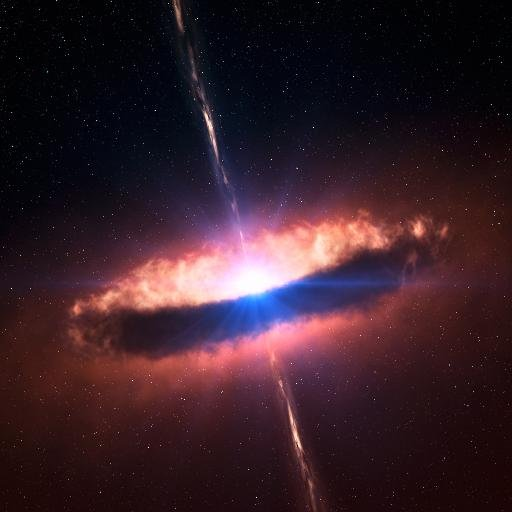
\includegraphics[width=0.3\textwidth]{Astrofysik/Astrofig/kvasarkunst.jpg}
		\caption{En kunstnerisk forestilling af en kvasar.} %https://pbs.twimg.com/profile_images/683524276058763264/xyAc-NvD.jpg
		\label{kvasarkunst}
	\end{figure}
	\begin{figure}[h!]
		\centering
		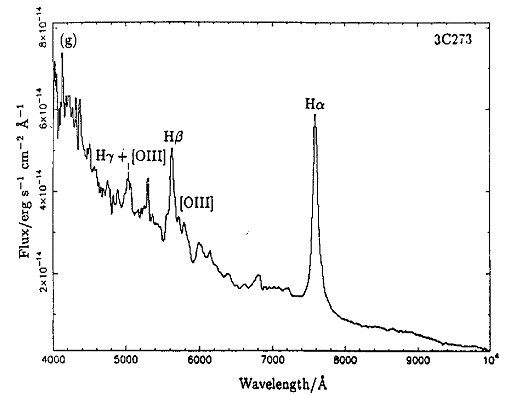
\includegraphics[width=0.5\textwidth]{Astrofysik/Astrofig/kvasar.png}
		\caption{ } %http://www.astrosurf.com/buil/us/spe6/qso1.gif
		\label{kvasar}
	\end{figure}
	\opg Ud fra din viden om H-$\alpha$-overgangen, bevæger kvasaren sig så mod eller væk fra os?
	\opg Hvad er kvasarens radielle hastighed?
	\opg Man ser tit, at spektrallinjerne fra kvasarer er meget brede, fordi gassen bevæger sig hurtigt omkring det sorte hul, hvilket giver en Doppler-forbredning
	(lyset bliver både rød- og blåforskudt). Estimér bredden af H-$\alpha$-linjen, $\Delta\lambda_{obs}$, og udregn gassens fart ved 
	\begin{align}
	v_{gas}=\frac{\Delta \lambda_{obs}}{2\lambda_{0}}c
	\end{align}
	Mål ca. halvvejs oppe, det behøver ikke være så præcist.
\end{opgave}
\begin{opgave}{Dopplerforskydning}{2}
	Formlen for frekvensen ved Dopplerforskydning er
	\begin{align}
		f_{obs} = \frac{c+v_{obs}}{c+v_{kilde}} f_{kilde},
	\end{align}
	hvor $c$ er lydens hastighed i mediet, $f_{obs}$ er den observerede frekvens (udefra), $f_{kilde}$ er den udsendte frekvens, $v_{obs}$ er observatørens hastighed og $v_{kilde}$ er kildens hastighed.
	\opg En politibil kører mod dig 30 meter væk, men er 20 meter fra centrum af vejen når du kigger ligeud (se skitsen på Figur \ref{politi}). Tegn hastighedsvektoren og hastighedskomponenterne der peger henholdsvis parallelt med din synsvinkel og vinkelret på den. Tænk over om den radielle hastighed er positiv eller negativ.
	\opg Bilens speedometer viser, at den kører 50 km/t. Brug trigonometri til at beregne hvor stor en hastighedskomponent, der peger mod dig (radiel hastighed). %Skitsér groft en graf over radiel hastighed som funktion af tid og antag, at bilens hastighed er konstant.
	\opg Politibilens sirene udsender lyd med en frekvens på 800 Hz. Du står stille, og det er en let kølig dag med 15 grader, hvor lydens fart i luft er 340 m/s. Ved hvilken frekvens hører du tonen?
	\begin{figure}[h!]
		\centering
		\includegraphics[width=0.5\textwidth]{Astrofysik/Astrofig/politi.png}
		\caption{ }
		\label{politi}
	\end{figure}
\end{opgave}
\begin{opgave}{Galaksen M87 i Virgohoben}{1}
	Galaksen M87 ligger i centrum af den nærmeste store
	galaksehob Virgohoben. Rødforskydningen af lys fra M87 og dermed fra centrum af
	Virgohoben er målt til $z = 0.00436$. Vi antager en Hubblekonstant på $H_0 = \SI{70}{\kilo\metre\per\second\per\mega\parsec}$.
	\opg Beregn afstanden til M87. Gør rede for dine antagelser. \\
	
	På vores teleskoper på Jorden modtager vi en samlet flux fra M87 på $f_\text{M87} = \SI{3.68e-12}{\watt\per\metre\squared}$.
	\opg Brug den information til at give et estimat over det totale antal stjerner i M87, idet vi
	antager, at de alle har samme luminositet som Solen, $L_\odot=\SI{3,839e26}{\watt}$.
\end{opgave}
\begin{opgave}{Afstandsbedømmelse i nabolaget}{2}
	En stjerne har en tilsyneladende magnitude på 17,5 og en absolut magnitude på -1,27.
	\opg Hvad er afstanden til stjernen? \\
	
	Hvis lysmængden fra et himmellegeme reduceres undervejs mod jorden, vil det se ud til at være længere væk, end det faktisk er. Det ses ved at den observerede flux mindskes, og den tilsyneladende magnitude stiger. Der gælder her at
	\begin{align*}
	m_{faktisk}-m_{obs} = -2,5 \log \left( \frac{f_{faktisk}}{f_{obs}} \right)
	\end{align*}
	\opg Det oplyses nu, at lyset på sin vej fra stjernen til os er blevet reduceret med 60\% pga. udslukning fra interstellart støv. Hvad er den faktiske afstand til stjernen?
\end{opgave}

\begin{opgave}{Afstande}{2}
	\\  
	\opg Opskriv luminositetsafstanden $D_L$ som funktion af vinkelafstanden $D_A$.
	\opg I et fladt univers er $D_M=D_C$. $D_C$ kaldes comoving distance, og med $\Omega_m=0.3$ og $\Omega_{\Lambda}=0.7$ opfører det sig som plottet på Figur \ref{comoving}. 
	Hvor stor er $D_L$ og $D_A$ ved $z=1$? \\
	Hvad med ved $z=9$? Giver ændringerne mening?
		\begin{figure}[h!]
			\centering
			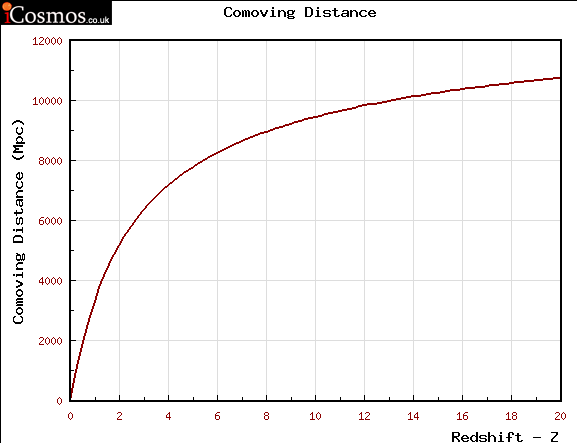
\includegraphics[width=0.5\textwidth]{Astrofysik/Astrofig/ComovingDistance.png}
			\caption{ } %http://www.icosmos.co.uk/index.html
			\label{comoving} 
		\end{figure}
	\opg Hvor stor er den radielle hastighed for et objekt med $z=10$? Oplys svaret som procent af lysets fart i vakuum. Dengang var universet for resten kun  478 mio. år gammelt.
\end{opgave}

\begin{opgave}{Himmellegemers overfladetemperatur}{3}
	Når et himmellegeme modtager stråling fra en nærliggende stjerne, vil noget af denne stråling reflekteres, og det bidrager derfor ikke til opvarmning af planeten. Albedoen $A$ er et tal fra 0 til 1 som angiver andelen af lyset, der reflekteres fra et objekt. 1 angiver 100 \% reflektion og derved at intet lys absorberes.
	\opg Vis først, at en planet eller måne med
	radius $R_m$ i en afstand $d$ (som luminositetsafstand) fra Solen og med en albedo-værdi på
	$A$ vil absorbere energien
	\begin{equation}
	L_\text{abs} = \frac{R_\odot^2\sigma T_\odot^4 \pi R_m^2}{d^2} \left( 1 - A \right),
	\end{equation}
	hvor $R_\odot$ og $T_\odot$ er hhv. radius og temperatur af Solen. \emph{Hint: man kan sige, at den del af planeten eller månen der er vendt mod Solen udgør et areal givet ved $\pi R_m^2$.} 
	\opg Hvis en måne eller planet roterer hurtigt, udsender den energi givet ved luminositeten $L_\text{uds}$ i ligning 1.25 i kompendiet. Solen er en stjerne i termisk ligevægt, så vi kan derfor skrive $L_\text{abs}=L_\text{uds}$. Vis, at temperaturen på overfladen af en planet eller måne, $T_m$, kan udtrykkes som
	\begin{equation}
	T_m = T_\odot \left( \frac{1-A}{4} \right)^{1/4} \left(\frac{R_\odot}{d} \right)^{1/2}
	\end{equation}
	\emph{Hint: start med at sætte $L_\text{abs}=L_\text{uds}$.} 
	\opg Saturns måne Mimas er placeret i en elliptisk bane omkring Saturn og  massen af Mimas er $M_\text{Mimas} = \SI{3,751e19}{\kilo\gram}$. Derudover er månens albedo $A_{Mimas} = 0,962$, mens Solens overfladetemperatur er $T_\odot = \SI{5778}{\kelvin}$, Solens radius er $R_\odot = \SI{6,955e5}{\kilo\metre}$, og middelafstanden mellem Mimas og Solen er $d_{\text{Mimas}} = \SI{1,43e9}{\kilo\metre}$. \\
	Beregn ud fra oplysningerne en teoretisk temperatur på overfladen af Mimas. Gøre rede for dine antagelser.
	\opg Cassini-rumsonden vurderede temperaturen på overfladen af Mimas til at være ca. \SI{65}{\kelvin} - hvad kan forskellen mellem den teoretiske og den observede temperatur skyldes?
\end{opgave}
\begin{opgave}{Skalafaktor}{1}
	Temperaturen af den kosmiske mikrobølgebaggrund er i dag 2.73 K. Strålingen blev udsendt ved "rekombinationen", hvor universet var koldt nok til at elektroner kunne binde sig til atomerne. Det var en mindre exciteret tilstand, så atomerne udsendte energi som fotoner. Man kan måle, at det har krævet en temperatur på maks 3000 K. Brug at temperaturen udviklede sig som
	\begin{align}
		T(t)=\frac{T_0}{a(t)}
	\end{align}
	til at finde ud af, ved hvilken rødforskydning rekombinationen fandt sted.
\end{opgave}

\begin{opgave}{Fladt univers med stof}{3}
	Forestil dig et fladt univers kun med stof.
	\opg Opskriv densitetsparametrene.
	\opg Opskriv skalafaktoren som funktion af tid.
	\opg Du står i nutiden $t_0 = 13,8$ mia. år og kigger på himlen. For en galakse med $z=1$, hvor længe skal du så observere den før rødforskydningen ændres med en $10^6$.-del? %Antag Hubblekonstanten er $H_0=70 km s^{-1} Mpc^{-1}$.
\end{opgave}

\begin{opgave}{Kosmologiske parametre}{3}
	%\opg Antag universet kun består af én komponent og er fladt. Hvordan afhænger denne komponents densitet af tiden? (Find $\rho(t)$) 
	\opg Opskriv Friedmannligningen, hvor du indsætter densiteterne af de forskellige komponenter. Se bort fra $\frac{\Lambda}{3}$-leddet, nu hvor du inkluderer densiteten af kosmologisk konstant i stedet.\\
	Hvad er $H^2$ som funktion af de nuværende værdier af parametrene?
	\opg Betragt nu vores univers, der er fladt. Hvornår bestod universet 50 \% af stråling og 50 \% stof? Mørk energi var der så lidt af, at det kunne negliceres dengang. Antag at skalafaktoren kun udvikler sig baseret på mængden af stråling og at universets nuværende alder er $13,8$ mia. år.
	\opg I virkeligheden sluttede den strålingsdominerede periode 47.000 år efter big bang. Hvorfor giver forrige delopgave noget andet?
	\opg Hvor meget kosmologisk konstant $\rho_\Lambda$ var der dengang? %Hvor stor en del af universet var kosmologisk konstant dengang?
\end{opgave}
\begin{opgave}{Andromeda-galaksen}{1}
	\begin{figure}[h!]
		\centering
		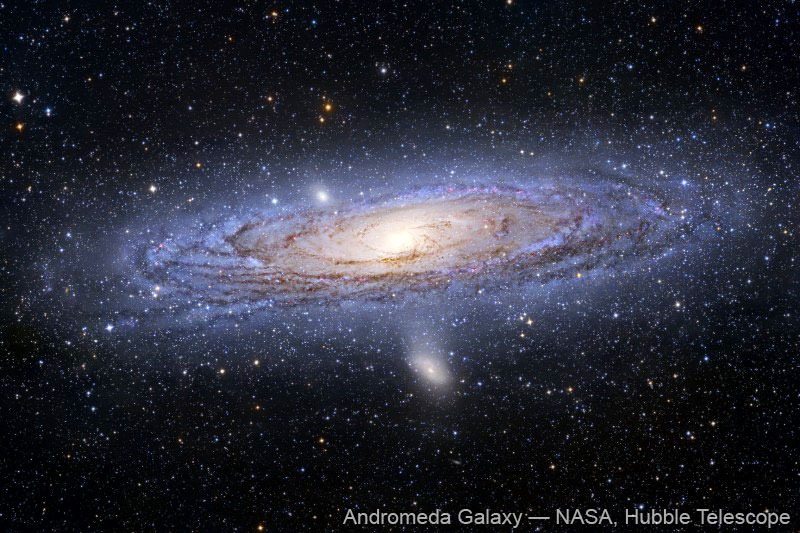
\includegraphics[width=0.5\textwidth]{Astrofysik/Astrofig/andromeda.jpg}
		\caption{  } %https://upload.wikimedia.org/wikipedia/commons/9/98/Andromeda_Galaxy_%28with_h-alpha%29.jpg
		\label{andromeda} 
	\end{figure}
	Andromeda-galaksen eller Messier-31 (M31) er den nærmeste spiralgalakse, og den største galakse i den Lokale Gruppe, som er en samling af ca. 50 galakser, heriblandt vores egen, Mælkevejen.  
	\opg Ligesom Mælkevejen er Andromedagalaksen en spiralgalakse, hvor alting kan antages at bevæge sig
	rundt om centrum i en cirkelbevægelse. Fra målinger på galaksen vurderes
	rotationshastigheden $v_{rot}(r)$ at vokse i de inderste få \SI{}{\kilo\parsec} fra centrum, hvorefter den flader ud
	og bliver konstant $v_{rot}(r) = v_{rot,max}$. Det vurderes, at $v_{rot,max} = \SI{230}{\kilo\metre\per\second}$. \\
	Giv et estimat af massen af Andromedagalaksen inden for radius $R = \SI{100}{\kilo\parsec}$ i enheder af Solens masse $M_\odot = \SI{1.9891e30}{\kilo\gram}$.
	\opg Det observerede lys fra Andromeda har en rødforskyning på $z = -0.001$.
	%\opg Det observerede lys fra Andromeda har en rødforskydning på $z = −0.001$.
	Hvad er Hubbleafstanden til galaksen, fundet ved hjælp af Hubbles lov? Antag Hubblekonstanten er $H_0=70 \text{km s}^{-1} \text{Mpc}^{-1}$.
	\opg Gennem andre metoder har man fundet afstanden til 2,5 mio. lysår. Hvornår støder Andromeda og Mælkevejen sammen? Hvad tror du, det kommer til at betyde? Antag hastigheden er konstant, og Andromeda har direkte kurs mod os.
\end{opgave}

\begin{opgave}{Betelgeuse}{1}
	Betelgeuse er en af de mest lysstærke stjerner på nattehimlen og findes i stjernebilledet Orion. Radius af Betelgeuse er målt til 1200
	gange Solens radius, $R_\odot=\SI{6,958e5}{\metre}$, med en overfladetemperatur på $T_B=\SI{3300}{\kelvin}$, mens Solens overfladetemperatur er $T_\odot=\SI{5778}{\kelvin}$. 
	\opg Bestem Solens og Betelgeuses luminositet i enheden \SI{}{\watt}, og enheder af Solens luminositet i tilfældet Betelgeuse.
	\opg Afstanden fra jorden til Betelgeuse er $d_B=\SI{642,5}{\lightyear}$. Bestem fluxen på jorden fra Betelgeuse og gør rede for nødvendige antagelser.
	\opg Afstanden fra jorden til Solen er $d_\odot=\SI{1}{AU}$. Hvor langt fra Betelgeuse er fluxen den samme, som fluxen fra solen er på jorden?
	\opg Voyager 1 satelitten er i dag $d_V=\SI{139}{AU}$ fra Solen og den stjerne, som er nærmest jorden, Proxima Centauri, befinder sig i afstanden $d_{PC}=\SI{4,3}{\lightyear}$. Hvordan er afstanden fra før sammenlignet med disse?
\end{opgave}

\begin{opgave}{Massen af Solsystemet}{1}
	Planeten Neptun, Solsystemets yderste planet, bevæger sig i en bane, der kan antages cirkulær, med  en baneradius på $R=\SI{30}{AU}$ og en periode på $P=\SI{164,8}{yr}$.
	\opg Bestem Neptuns gennemsnitlige banefart idet perioden er tiden det tager at gennemløbe cirkelbanen.
	\opg Estimer den totale masse af solsystemet og sammenlign med Solens masse.
\end{opgave}
%\begin{opgave}{Mere filosofiske spørgsmål}{1}
%	\opg Mange parametre og konstanter i universet har akkurat værdier, der tillader os at eksistere. Det fremkommer usandsynligt bare at have et univers, der ikke går under på et splitsekund og indeholder stabil masse. Hvor mange mulige forklaringer kan du komme med?
%	\opg Mælkevejen er et stort sted og
%\end{opgave}

\chapter{Astrofysik Facitliste}
\section*{Astrofysik}
\begin{opgave}{Rødforskydning af kvasar}{2}
	\opg nm er $10^{-9} m= 10 \cdot 10^{-10}$, så H-$\alpha$-linjen er ved ca. $6560$ Å. På figuren er det ved omkring $7600$ Å, dvs. bølgelængden er blevet større, så lyset er rødforskudt. Altså må kvasaren bevæge sig væk fra os.\\
	\opg Den radielle hastighed er beskrevet af rødforskydningen. Rødforskydningen er
	\begin{align}
	\frac{\lambda_{obs}-\lambda_{lab}}{\lambda_{lab}} = \frac{7600-6560}{6560} = 0,159.
	\end{align}
	Det er lavt, så vi approksimerer hastigheden til
	\begin{align}
	v= z*c = 0,159 \cdot 3\cdot 10^8 = 4,7*10^7 m/s
	\end{align}
	Regner du det præcist, giver det nogenlunde det samme.
	\opg $\Delta\lambda \approx 200 Å$, så det giver $v=0.015 c = 4,5*10^6 m/s$.
\end{opgave}

\begin{opgave}{Dopplerforskydning}{1}
	\opg 
	\begin{figure}[h!]
		\centering
		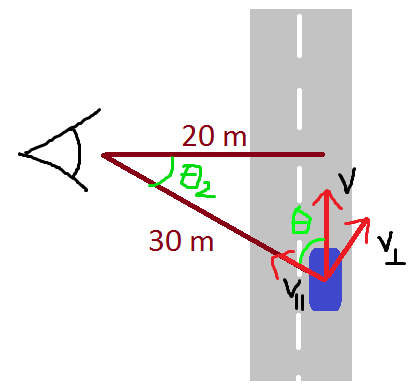
\includegraphics[width=0.5\textwidth]{Astrofysik/Astrofig/PolitiLoesning.png}
		%\caption{Et typisk } %https://upload.wikimedia.org/wikipedia/commons/9/98/Andromeda_Galaxy_%28with_h-alpha%29.jpg
	\end{figure}
	\opg Den radielle hastighed er den parallele komponent med synsvinklen. Vi ser en retvinklet trekant og bruger
	\begin{align}
		cos(\theta)=\frac{\text{hosliggende katete}}{\text{hypotenusen}}=\frac{v_{radiel}}{v} \\
		v_{radiel}=v cos(\theta)
	\end{align}
	Der dannes også en retvinklet trekant af vejen, afstanden til vejen og afstanden til bilen. I grader giver det en vinkel på
	\begin{align}
		cos(\theta_2)&=\frac{20}{30}\\
		\theta_2 &= cos^{-1} \left( \frac{20}{30} \right) = 48
	\end{align}
	De to vinkler indgår begge i en retvinklet trekant, så
	\begin{align}
		180 &= \theta + \theta_2 + 90\\
		\theta &= 90 - \theta_2  = 42
	\end{align}
	Vi indsætter og får
	\begin{align}
	v_{radiel}=50 km/t * cos(42) = 50 km/t * 0.74 = 37 km/t
	\end{align}
	Hvis du ikke får det samme, så prøv at regne alt i radianer, da det er simplere.
	\opg 
	Du står stille, så $v_{obs}=0$. $v_{kilde}$ er den radielle hastighed, som lige skal omregnes til km/t:
	\begin{align}
	37 km/t = 37 \frac{10^{3}m}{60*60 s} = \frac{37}{3.6} m/s = 10,3 m/s
	\end{align}
	Så indsætter vi i
	\begin{align}
	f_{obs} = \frac{340 m/s + 0}{340 m/s - 10,3} 800 Hz = 825 Hz
	\end{align}
	Bemærk hastigheden er negativ i forhold til observatøren.
\end{opgave}
\begin{opgave}{Galaksen M87 i Virgohoben}{1}
	\opg Hubble loven giver, under antagelse af at M87 bevæger sig væk fra jorden som følge af universets udvidelse, at
	\begin{align*}
	v = H_0D
	\end{align*}
	Idet $z<<1$ kan den ikke relativistiske approksimation benyttes
	\begin{align*}
	z\approx\frac{v}{c}
	\end{align*}
	Komineres de to ligninger fås
	\begin{align*}
	D_\text{M87} = \frac{zc}{H_0} = \SI{18,7}{\mega\parsec}
	\end{align*}
	\opg Under antagelse af at strålingen er udsendt isotropt fra M87, så den samlede luminositet
	\begin{align*}
	L_\text{M87} = 4\pi D_\text{M87}^2\cdot f_\text{M87}
	\end{align*}
	Estimatet for antallet af stjerner i M87, $N_\text{M87}$, bliver så
	\begin{align*}
	N_\text{M87} = \frac{L_\text{M87}}{L_\odot} = \SI{4,01e10}{}
	\end{align*}
\end{opgave}
\begin{opgave}{Afstandsbedømmelse i nabolaget}{1}
	\opg Vi ved at
	\begin{align*}
	m-M = 5\log \left( \frac{d_L}{\si{pc}} \right) -5
	\end{align*}
	Og vi vil gerne bestemme $d_L$, så den isoleres. 
	\begin{align*}
	\frac{m-M+5}{5} &= \log \left( \frac{d_L}{\si{pc}} \right) \\
	\Rightarrow 10^{\frac{m-M+5}{5}} &= 10^{\log \left( \frac{d_L}{\si{pc}} \right)}\\
	&= \frac{d_L}{\si{pc}}\\
	\Rightarrow d_L &= 10^{\frac{m-M+5}{5}}\\
	& \approx 56754~\si{pc}
	\end{align*}
	\opg Hvis udslukningen er 60$\%$ vil kun 40 $\%$ af lyset nå os. Det betyder også at 
	\begin{align*}
	0,40f_{faktisk} &= f_{obs}\\
	f_{faktisk} &= \frac{f_{obs}}{0,40}
	\end{align*}
	Vi har nu udtrykket 
	\begin{align*}
	m_1-m_2 = -2,5 \log \left( \frac{f_1}{f_2} \right) 
	\end{align*}	 
	Hvor $f_1$ erstattes med med $f_{faktisk}$. 
	\begin{align*}
	m_{faktisk}-m_{obs} = -2,5 \log \left( \frac{f_{obs}}{0,40f_{obs}} \right) 
	\end{align*}
	Det betyder
	\begin{align*}
	m_{faktisk} &=-2,5\log \left( \frac{1}{0,40} \right) +m_{obs} \\
	&= 16,5
	\end{align*}
	En mindre magnitude betyder, at stjernen lyser klarere. \\
	Så for at bestemme den faktisk afstand indsættes den faktiske tilsyneladende magnitude i udtrykket fra delopgave 1. 
	\begin{align*}
	d_{faktisk} = 35809~\si{pc}
	\end{align*}
\end{opgave} 
\begin{opgave}{Afstande}{1}
	\opg Isolér $D_M$ i hvert udtryk.
	\begin{align}
		D_M &= \frac{D_L}{1+z}\\
		D_M &= D_A(1+z)
	\end{align}
	Resultaterne sættes lig hinanden
		\begin{align}
		\frac{D_L}{1+z} &= D_A(1+z)\\
		D_L &= D_A (1+z)^2
		\end{align}
	\opg Ved $z=1$ er $D_C\approx3200 Mpc$ og derfor
	\begin{align}
		D_L &= D_M(1+z)= 3200 Mpc \cdot 2 = 6400 Mpc\\
		D_A &= \frac{D_M}{1+z}= 3200 Mpc/ 2 = 1600 Mpc.
	\end{align}
	Ved $z=9$ er $D_C\approx9200 Mpc$, så
	\begin{align}
		D_L &= D_M(1+z)= 9200 Mpc \cdot 10 = 92000 Mpc\\
		D_A &= \frac{D_M}{1+z}= 9200 Mpc/ 10 = 920 Mpc.
	\end{align}
	Gamle objekter, der har bevæget sig fra os længere tid, har altså en større luminositetsafstand, men en lavere vinkelafstand ved høje rødforskydninger. Man skulle ellers tro objekter så mindre ud på himlen, jo længere væk de var, hvilket er rigtigt indtil omkring $z=1,6$. I det tidlige univers var galakserne tættere på hinanden, så de fyldte meget på himlen for hinanden, og derfor er deres lys spredt ud over et stort område.
	\opg
	%Dengang var universet for resten kun 250 mio. år gammelt.\\
	Hvis vi approksimerer $z\approx\frac{v}{c}$, får vi overlyshastigheder, så det går ikke.
	\begin{align}
	z+1&=\sqrt{\frac{1+\frac{v}{c}}{1-\frac{v}{c}}}\\
	(z+1)^2&=\frac{1+\frac{v}{c}}{1-\frac{v}{c}}
	\end{align}
	så vi skal løse et system på formen $y=\frac{1+x}{1-x}$, hvor $y=(z+1)^2$ og $x=\frac{v}{c}$. Man kan omformulere det til $x=\frac{y-1}{y+1}$. Derfor må
	\begin{align}
	\frac{v}{c}&=\frac{(z+1)^2-1}{(z+1)^2+1}\\
	v&=\frac{(z+1)^2-1}{(z+1)^2+1} c = \frac{(10+1)^2-1}{(10+1)^2+1} = 0,98 c. %3\cdot 10^{8} m/s =
	\end{align}
	Så svaret er 98 \% af lysets fart i vakuum.
\end{opgave}
\begin{opgave}{Himmellegemers overfladetemperatur}{3}
	\opg For at kunne komme frem til udtrykket starter vi med at se på fluxen, altså det lys, som vi modtager. Fluxen er givet ved
	\begin{align*}
	f &= \frac{L_\odot}{4\pi d^2}\\
	&= \frac{4\pi R_\odot^2 \sigma T_\odot^4}{4\pi d^2}\\
	&= \left( \frac{R_\odot}{d}\right) ^2 \sigma T_\odot^4
	\end{align*}
	Vi ser nu på den energi som planeten absorberer. Vi antager at vi har en jævn kugle, som energien fordeles jævnt udover. Derudover skal vi have albedoen i spil, i det den fortæller os hvor meget lys, der bliver reflekteret. 
	\begin{align*}
	L_\text{abs} &= \pi R_{m}^2 f \left( 1-A\right) \\
	&= \pi R_{m}^2 \left( \frac{R_\odot}{d}\right) ^2 \sigma T_\odot^4 \left( 1-A\right)\\
	&= \frac{\pi R_m^2R_\odot^2 \sigma T_\odot^4}{d^2} \left( 1-A\right) 
	\end{align*}
	\opg I det Solen er en stjerne i termisk ligevægt, det betyder at der bliver udsendt lige så meget energi som der bliver absorberet. 
	\begin{align*}
	L_\text{uds} = 4\pi R_m^2 \sigma T_m^4
	\end{align*}
	\begin{align*}
	L_\text{uds} &= L_\text{abs} \\
	\Rightarrow 4\pi R_m^2 \sigma T_m^4 &= \frac{\pi R_m^2R_\odot^2 \sigma T_\odot^4}{d^2} \left( 1-A\right) \\
	\Rightarrow 4T_m^4 &= \left( \frac{R_\odot}{d} \right) ^2 T_\odot^4 \left( 1-A\right) \\
	\Rightarrow T_m^4 &= \left( \frac{R_\odot}{d} \right) ^2 \frac{\left( 1-A\right)}{4} T_\odot^4\\ 
	\Rightarrow T_m &= \left( \frac{R_\odot}{d} \right) ^{\frac{1}{2}} \left( \frac{\left( 1-A \right) }{4} \right) ^{\frac{1}{4}} T_\odot
	\end{align*}
	\opg Vi bruger udtrykket, som vi lige har fundet og bestemmer temperaturen på overfladen. 
	\begin{align*}
	T_m \approx \SI{40}{\kelvin}
	\end{align*}
	\opg Vi antager at Mimas roterer hurtigt. Det har den betydning, at vi antager at temperaturen er den samme på over det hele, der vil altså ikke være noget ''dag og nat''. Den teoretiske værdi er bestemt til \SI{40}{\kelvin} og temperaturen er blevet vurderet til \SI{65}{\kelvin}. Det tyder derfor på, at vores antagelse om hurtigt rotation muligvis ikke er så god. Hvis den roterer langsomt, vil det betyde at temperaturen ikke er den samme overalt, hvilket kan forklare hvorfor temperaturen er blevet vurderet til \SI{65}{\kelvin}. 
\end{opgave}
\begin{opgave}{Skalafaktor}{2}
	\opg Vi omskriver formlen og indsætter temperaturerne
		\begin{align}
		a(t)=\frac{T_0}{T(t)}\\
		a(t)=\frac{2.73 K}{3000 K} \approx 10^{-3}
		\end{align}
		Så kan denne formel bruges:
		\begin{align}
		a(t) = \frac{1}{1+z}\\
		z = \frac{1}{a(t)} - 1\\
		z = \frac{1}{10^{-3}} - 1 \approx 10^3
		\end{align}
		Så rekombinationen skete ved $z\approx 1000$.
\end{opgave}
\begin{opgave}{Fladt univers med stof}{2}
	\opg Hvis universet er fladt, er $\Omega_{total}=1$. Består det kun af stof, må $\Omega_m=1$ og resten er 0.
	\opg Skalafaktoren er
	\begin{align}
	a(t)=\left(\frac{t}{t_0}\right)^{2/(3+3\omega)} = \left(\frac{t}{t_0}\right)^{2/3}
	\end{align}
	da $\omega=0$ for stof.
	\opg En $10^6.$-del af 1 er $10^{-6}$. Baseret på $z=\frac{a(t_0)}{a(t)}-1$ kan ændring i rødforskydning opskrives
	\begin{align}
		\Delta z =|\frac{a(t_0)}{a(t_0)} - \frac{a(t_0)}{a(t_1)}|= |1-\frac{1}{a(t_1)}|\\
		%\Delta z &= |1-\frac{1}{a(t_1)}|
		 %\sqrt{\frac{1+\frac{\Delta v}{c}}{1-\frac{\Delta v}{c}}} - 1
	\end{align}
	hvor vi sætter $a(t_0)=1$ og $t_1$ er tidspunktet, vi stopper med at observere. Det ligger efter $t_0$, så $|1-\frac{1}{a(t_1)}|=1 - \frac{1}{a(t_1)}$
	Vi isolerer $a(t_1)$ 
	\begin{align}
	a(t_1) = \frac{1}{1-\Delta z} &= \left(\frac{t_1}{t_0}\right)^{2/3} \\
	\frac{t_1}{t_0} &= \left( \frac{1}{1-\Delta z} \right)^{3/2}
	%t_1 &= \left( \frac{1}{\Delta z + 2} \right)^{3/2} t_0
	\end{align}
	Vi indsætter ændringen i $z$
		\begin{align}
		\frac{t_1}{t_0} &= \left( \frac{1}{1-10^{-6}} \right)^{3/2} = 1.0000015
		%t_1 &= \left( \frac{1}{\Delta z + 2} \right)^{3/2} t_0
		\end{align}
	Så vi skal vente til tidspunktet $t_1 = t_0 + \Delta t = 1.0000015*t_0$, hvor $t_0$ er universets nuværende alder.
	\begin{align}
		\Delta t = (1.0000015 - 1) t_0 = 0.0000015 t_0 = 0.0000015*13.8*10^{9} \text{år} - = 20700 \text{år}
	\end{align}
\end{opgave}
\begin{opgave}{Kosmologiske parametre}{0}
	\opg 
	\begin{align}
	H^2=\frac{8\pi G \rho}{3}-\frac{\kappa c^2}{a^2}+\frac{\Lambda}{3}.
	\end{align}
	bliver til
	\begin{align}
	H^2=\frac{8\pi G}{3} (\rho_R+\rho_m+\rho_\Lambda)-\frac{\kappa c^2}{a^2} 
	\end{align}
	Så bruger vi $\rho_R=\rho_{R,0}a(t)^{-4}, \rho_m=\rho_{m,0}a(t)^{-3}$ og $\rho_\Lambda=\rho_{\Lambda,0}$ :
	\begin{align}
	H^2=\frac{8\pi G}{3} (\frac{\rho_{R,0}}{a(t)^4}+\frac{\rho_{m,0}}{a(t)^3}+\rho_\Lambda)-\frac{\kappa c^2}{a^2} 
	\end{align}
	\opg
	Bidraget fra stråling skal være lige så stort som det for stof
	\begin{align}
	\rho_R &= \rho_m\\
	\frac{\rho_{R,0}}{a(t)^4} &= \frac{\rho_{m,0}}{a(t)^3}\\
	\rho_{m,0} a(t) &= \rho_{R,0}\\
	a(t) &= \frac{\rho_{R,0}}{\rho_{m,0}} = 0.000267
	\end{align}
	Så bruger vi
	\begin{align}
		a(t)=\left(\frac{t}{t_0}\right)^{2/(3+3\omega)} = \left(\frac{t}{t_0}\right)^{1/2}\\
		t = a(t)^2 t_0 = 0.000267^2 \cdot 13.8\cdot10^9 \text{år} = 982 \text{år}
	\end{align}
	\opg Det giver noget ca. 50 gange for lavt, da det er en dårlig approksimation at antage universets størrelse udvikler sig som om det består af stråling. Stof og mørk energi har enorm betydning for universets alder $t_0$.
	\opg Mængden af kosmologisk konstant er konstant.
	\begin{align}
		\rho_\Lambda = \Omega_\Lambda \rho_c = 0.6911 \cdot 8.6\cdot 10^{-27} kg/m^3 = 5.9 \cdot 10^{-27} kg/m^3
	\end{align}
	\iffalse % Udkommentering
	Vi kender for stof og stråling
	\begin{align}
		\rho = \rho_0 a^{-3(1+\omega)}
	\end{align}
	 og indsætter $a(t)=\left(\frac{t}{t_0}\right)^{2/(3+3\omega)}$
	 \begin{align}
	 \rho = \rho_0 \left(\left(\frac{t}{t_0}\right)^{2/(3+3\omega)}\right)^{-3(1+\omega)} = \rho_0 \left(\frac{t}{t_0}\right)^{-6(1+\omega)/(3+3\omega)}
	 = \rho_0 \left(\frac{t}{t_0}\right)^{-2} \propto t^{-2}.
	 \end{align}
	 For kosmologisk konstant
	 	\begin{align}
		 	\rho = \rho_0 a^0 = \rho_0 % = \rho_0 e^{H_0(t-t_0)} \propto e^{H_0t}
	 	\end{align}
	 \opg Hvis vi ignorerer kosmologisk konstant, leder vi efter tidspunktet hvor $\Omega_R = 0,9$ og $\Omega_R = 0,1$. Vi husker $\Omega_R=\frac{\rho_R}{\rho_c}$, så vi søger tidspunktet hvor
	 \begin{align}
	 	\rho_R &= \Omega_R \rho_c = 0,9 \cdot 8,6 \cdot 10^{-27}kg/m3 = 7.74 \cdot  10^{-27}kg/m3\\
	 	\rho_m &= \Omega_m \rho_c = 0,1 \cdot 8,6 \cdot 10^{-27}kg/m3 = 0.86 \cdot  10^{-27}kg/m3.
	 \end{align}
	 Vi kender de nuværende værdier, så tidspunktet kan findes ved
	 \begin{align}
	 	t=(\rho_R/\rho_{R,0})^{-1/2} = (\rho_m/\rho_{m,0})^{-1/2}\\
	 	=(\Omega_R/\Omega_{R,0})^{-1/2} = (\Omega_m/\Omega_{m,0})^{-1/2}
	 	=
	 \end{align}
	 %Nej, regn a først, det her giver 2 forskellige ting
	 \fi
\end{opgave}
\begin{opgave}{Andromeda-galaksen}{2}
	\opg Ligning 1.22 i kompendiet giver at
	\begin{align*}
	v^2 = \frac{GM(R)}{R}
	\end{align*}
	Her isoleres $M(R)$ som er massen af af den del af Andromeda-galaksen, som ligger indenfor afstanden $R$ fra centrum, og de opgivne værdier indsættes
	\begin{align*}
	M(R) = \frac{v^2R}{G} = \SI{2,45e42}{\kilo\gram} = \SI{1,23e12}{M_\odot}
	\end{align*}
	\opg 
	\begin{align}
	D_H=\frac{v}{H_0} 
	\end{align}
	Vi skal bruge den radielle hastighed
	\begin{align}
	v \approx z c = -0.001 \cdot 3\cdot 10^8 m/s =-3\cdot 10^5 m/s
	\end{align}
	og omskriver Hubble-konstanten en lille smule
	\begin{align}
	H_0=70 km s^{-1} Mpc^{-1} = 7 \cdot 10^4 m s^{-1} Mpc^{-1}.
	\end{align}
	Vi indsætter
	\begin{align}
	D_H=\frac{-3\cdot 10^5 m s^{-1}} {7 \cdot 10^4 m s^{-1} Mpc^{-1}} = - 3/7 \cdot 10 Mpc = - 4,2 Mpc.
	\end{align}
	Så Hubble-afstanden bryder sammen og giver noget negativt.
	\opg Vi omregner lysår til meter
	\begin{align}
	2.5\cdot 10^6 \text{lysår} = 2.5\cdot 10^6 \cdot 9,46 \cdot 10^15 m = 23.7 \cdot 10^21 m\\
	\frac{23.7 \cdot 10^21 m}{3\cdot 10^5 m/s} = 7.9 \cdot 10^16 s = 2,5 \cdot 10^9 \text{år}
	\end{align} 
	Så det vil tage 2,5 mia. år, hvis vi ser bort fra accelerationen og andre effekter. I virkeligheden er det 4-5 mia. år.
	Stjernerne er ligger meget spredt i begge galakser, så vi kommer ikke til at støde ind i andre. Når gassen fra galakserne kolliderer varmes det op og vi vil se en masse ny stjernedannelse. Galakserne vil med tiden smelte sammen til en elliptisk galakse, der har opbrugt det meste gas, så der ikke dannes flere stjerner. 
\end{opgave}

\begin{opgave}{Betelgeuse}{1}
	\opg Hvis vi antager at Betelgeuse er et sfærisk sortlegeme, der udsender sortlegemestråling kan vi beregne dens luminositet vha. formel (1.25) fra kompendiet
	\begin{align*}
	L_\odot &= 4\pi R_\odot^2\sigma T_\odot^4 =\SI{3.839e26}{\watt} \\
	L_B &= 4\pi R_B^2\sigma T_B^4 =\SI{5,886e31}{\watt} = \SI{1,533e5}{L_\odot}
	\end{align*}
	\opg Fluxen fra et isotropt udstrålende stortlegeme er ved negligering af ekstinktion
	\begin{align*}
	f_B = \frac{L_B}{4\pi d_B^2} = \SI{1,27e-7}{\watt\per\metre\squared}
	\end{align*}
	\opg Fluxen fra solen på jorden, $L_\odot$ er, under samme antagelser som før, givet som
	\begin{align*}
	f_\odot = \frac{L_\odot}{4\pi d_\odot^2}
	\end{align*}
	hvorfor
	\begin{align*}
	f_\odot = f \quad&\Rightarrow\quad \frac{L_\odot}{4\pi d_\odot^2} = \frac{L_B}{4\pi d^2} \\
	\Rightarrow\quad d &= \sqrt{\frac{L_B}{L_\odot}d_\odot} = \SI{392}{AU}
	\end{align*}
	\opg Idet $d\approx2.8\cdot d_V$ ville man skulle næsten 3 gange længere væk fra Betelgeuse end Voyager 1 er fra Solen, hvilket er en afstand meget større end solsystemes radius, da Voyager 1 er omkring udkanten af solsystemet. Afstanden er dog ikke sammenlignelige med den til Proxima Centauri, fordi $d$ ca. er 1.4\permil af $d_{PC}$.
\end{opgave}
\begin{opgave}{Massen af Solsystemet}{1}
	\opg Idet Neptuns bane er antaget cirkulær er den tilbagelagte afstand, $D$, iløbet af én periode
	\begin{align*}
	D = 2\pi R
	\end{align*}
	hvorved den gennemsnitlige banefart bliver
	\begin{align*}
	v = \frac{d}{P} = \frac{2\pi R}{P} = \SI{5,42}{\kilo\metre\per\second}
	\end{align*}
	\opg For himmelegemer i cirkulære baner er
	\begin{align*}
	v^2 = \frac{GM(R)}{R}
	\end{align*}
	hvorved massen af solsystemet approksimeres til
	\begin{align*}
	M(R) = \frac{Rv^2}{G} = \frac{4\pi^2R^3}{GP^2} = \SI{0,994}{M_\odot}
	\end{align*}
\end{opgave}


\begin{opgave}{Dopplerforskydning}{2}
	Formlen for frekvensen ved Dopplerforskydning er
	\begin{align}
		f_{obs} = \frac{c+v_{obs}}{c+v_{kilde}} f_{kilde},
	\end{align}
	hvor $c$ er lydens hastighed i mediet, $f_{obs}$ er den observerede frekvens (udefra), $f_{kilde}$ er den udsendte frekvens, $v_{obs}$ er observatørens hastighed og $v_{kilde}$ er kildens hastighed.
	\opg En politibil kører mod dig 30 meter væk, men er 20 meter fra centrum af vejen når du kigger ligeud. Tegn hastighedsvektoren og hastighedskomponenterne der peger henholdsvis parallelt med din synsvinkel og vinkelret på den. 
	\opg Bilens speedometer viser, at den kører 50 km/t. Brug trigonometri til at beregne hvor stor en hastighedskomponent, der peger mod dig (radiel hastighed). Skitsér groft en graf over radiel hastighed som funktion af tid og antag, at bilens hastighed er konstant.
	\opg Politibilens sirene udsender lyd med en frekvens på 800 Hz. Du står stille, og det er en let kølig dag med 15 grader, hvor lydens fart i luft er 340 m/s. Ved hvilken frekvens hører du tonen?
	\begin{figure}[h!]
		\centering
		\includegraphics[width=0.5\textwidth]{Astrofysik/Astrofig/politi.png}
		%\caption{Et typisk }
		\label{politi}
	\end{figure}
\end{opgave}

\begin{opgave}{Rødforskydning af kvasar}{1}
	Kvasarer (eng:”quasars” fra ”quasi-stellar radio sources”) er de mest energirige og
	fjerne medlemmer af objekterne kendt som aktive galaksekerner (eng:”AGN: Active
	Galactic Nuclei”). Kvasarer har siden deres opdagelse været omgivet af mystik, men
	der er nu opnået generel enighed om, at de er kompakte regioner i massive galakser,
	der indeholder det centrale supermassive sorte hul. De kæmpe mængder energi der
	bliver udstrålet af kvasarerne stammer fra al stoffet, som falder ind mod det sorte
	hul og bliver slynget ud.
	Et kvasar-spektrum er vist i Figur \ref{kvasar}.
	\\
	I Balmer-serien hopper en elektron til 2. orbital fra en mere exciteret tilstand. Den første af disse kaldes H-$\alpha$ og er faldet fra orbital 3 til 2. Den næste er H-$beta$ fra orbital 4 til 2 osv. Fotoner, der udsendes ved H-$\alpha$-overgangen, har en bølgelængde på 656 nm. Ofte måler man i ångstrøm (Å) som er $10^{-10}$ m.\\
	%Aflæs bølgelængden for H-$\beta$ på Figur \ref{spektrum} og beregn rødforskydningen.
		\begin{figure}[h!]
			\centering
			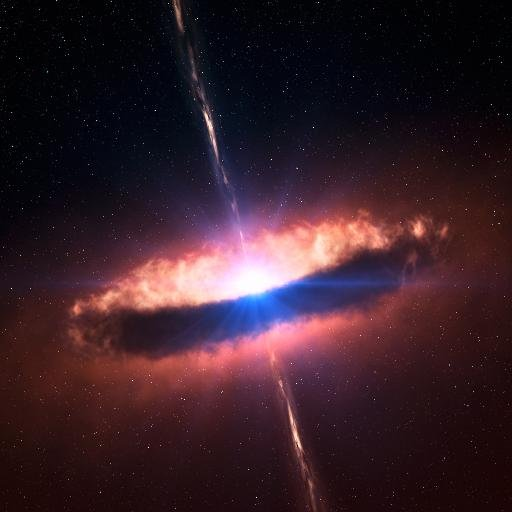
\includegraphics[width=0.5\textwidth]{Astrofysik/Astrofig/kvasarkunst.jpg}
			\caption{En kunstnerisk forestilling af en kvasar.} %https://pbs.twimg.com/profile_images/683524276058763264/xyAc-NvD.jpg
			\label{kvasarkunst}
		\end{figure}
	\begin{figure}[h!]
		\centering
		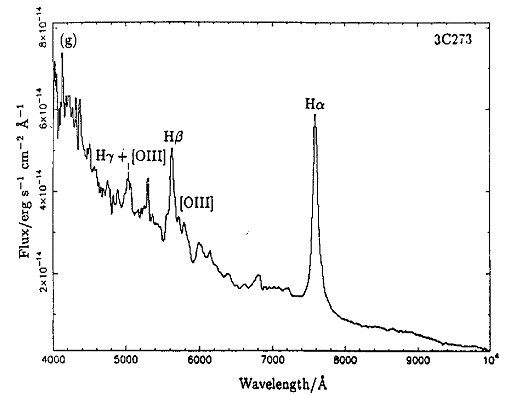
\includegraphics[width=0.5\textwidth]{Astrofysik/Astrofig/kvasar.png}
		%\caption{} %http://www.astrosurf.com/buil/us/spe6/qso1.gif
		\label{kvasar}
	\end{figure}
	\opg Ud fra din viden om H-$\alpha$-overgangen, bevæger kvasaren sig så mod eller væk fra os?
	\opg Hvad er kvasarens radielle hastighed?
	\opg Man ser tit, at spektrallinjerne fra kvasarer er meget brede, fordi gassen bevæger sig hurtigt omkring det sorte hul, hvilket giver en Doppler-forbredning
	(lyset bliver både rød- og blåforskudt). Estimér bredden af H-$\alpha$-linjen, $\Delta\lambda_{obs}$, og udregn gassens fart ved 
	\begin{align}
		v_{gas}=\frac{\Delta \lambda_{obs}}{2\lambda_{0}}c
	\end{align}
\end{opgave}

\begin{opgave}{Afstande}{3}
	\\  
	\opg Opskriv luminositetsafstanden $D_L$ som funktion af vinkelafstanden $D_A$.
	\opg I et fladt univers er $D_M=D_C$. $D_C$ kaldes comoving distance, og med $\Omega_m=0.3$ og $\Omega_{\Lambda}=0.7$ opfører det sig som plottet på Figur \ref{comoving}. 
	Hvor stor er $D_L$ og $D_A$ ved $z=1$? \\
	Hvad med ved $z=9$? Giver ændringerne mening?
		\begin{figure}[h!]
			\centering
			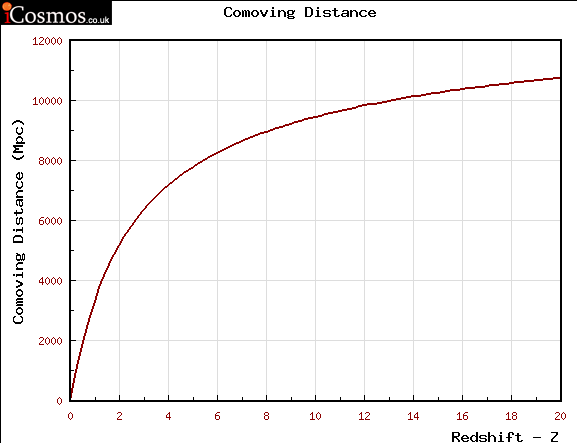
\includegraphics[width=0.5\textwidth]{Astrofysik/Astrofig/ComovingDistance.png}
			%\caption{Et typisk } %http://www.icosmos.co.uk/index.html
			\label{comoving} 
		\end{figure}
	\opg Hvor stor er den radielle hastighed for et objekt med $z=10$? Oplys svaret som procent af lysets fart i vakuum. Dengang var universet for resten kun  478 mio. år gammelt.
\end{opgave}

\begin{opgave}{Andromeda-galaksen}{2}
		\begin{figure}[h!]
			\centering
			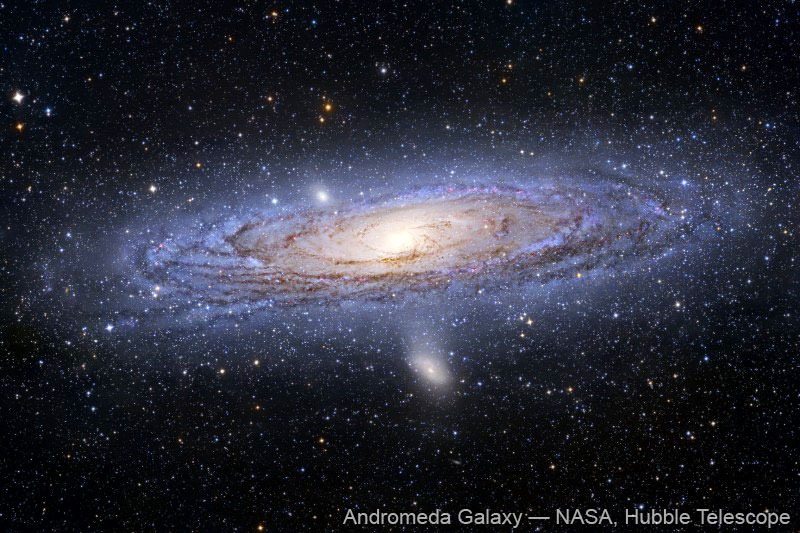
\includegraphics[width=0.5\textwidth]{Astrofysik/Astrofig/andromeda.jpg}
			%\caption{Et typisk } %https://upload.wikimedia.org/wikipedia/commons/9/98/Andromeda_Galaxy_%28with_h-alpha%29.jpg
			\label{andromeda} 
		\end{figure}
	Andromeda-galaksen eller Messier-31 (M31) er den nærmeste spiralgalakse, og den største galakse i den Lokale Gruppe, som er en samling af ca. 50 galakser, heriblandt vores egen, Mælkevejen.  
	\opg Det observerede lys fra Andromeda har en rødforskyning på $z = -0.001$.
	%\opg Det observerede lys fra Andromeda har en rødforskydning på $z = −0.001$.
	Hvad er Hubbleafstanden til galaksen, fundet ved hjælp af Hubbles lov? Antag Hubblekonstanten er $H_0=70 km s^{-1} Mpc^{-1}$.
	\opg Gennem andre metoder har man fundet afstanden til 2,5 mio. lysår. Hvornår støder Andromeda og Mælkevejen sammen? Hvad tror du, det kommer til at betyde? Antag hastigheden er konstant, og Andromeda har direkte kurs mod os.
\end{opgave}

\begin{opgave}{Skalafaktor}{1}
	Temperaturen af den kosmiske mikrobølgebaggrund er i dag 2.73 K. Strålingen blev udsendt ved "rekombinationen", hvor universet var koldt nok til at elektroner kunne binde sig til atomerne. Det var en mindre exciteret tilstand, så atomerne udsendte energi som fotoner. Man kan måle, at det har krævet en temperatur på kun 3000 K. Brug at temperaturen udviklede sig som
	\begin{align}
		T(t)=\frac{T_0}{a(t)}
	\end{align}
	til at finde ud af, ved hvilken rødforskydning rekombinationen fandt sted.
\end{opgave}

\begin{opgave}{Fladt univers med stof}{2}
	Forestil dig et fladt univers kun med stof.
	\opg Opskriv densitetsparametrene.
	\opg Opskriv skalafaktoren som funktion af tid.
	\opg Antag Hubblekonstanten er $H_0=70 km s^{-1} Mpc^{-1}$. For en galakse med $z=1$, hvor længe skal du så observere den før rødforskydningen ændres med en $10^6$.-del?
\end{opgave}

\chapter{Astrofysik Facitliste}
\section*{Astrofysik}
\begin{opgave}{Dopplerforskydning}{1}
	\opg 
	\begin{figure}[h!]
		\centering
		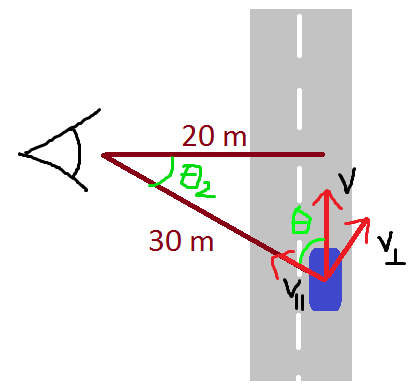
\includegraphics[width=0.5\textwidth]{Astrofysik/Astrofig/PolitiLoesning.png}
		%\caption{Et typisk } %https://upload.wikimedia.org/wikipedia/commons/9/98/Andromeda_Galaxy_%28with_h-alpha%29.jpg
	\end{figure}
	\opg Den radielle hastighed er den parallele komponent med synsvinklen. Vi ser en retvinklet trekant og bruger
	\begin{align}
		cos(\theta)=\frac{\text{hosliggende katete}}{\text{hypotenusen}}=\frac{v_{radiel}}{v} \\
		v_{radiel}=v cos(\theta)
	\end{align}
	Der dannes også en retvinklet trekant af vejen, afstanden til vejen og afstanden til bilen. I grader giver det en vinkel på
	\begin{align}
		cos(\theta_2)&=\frac{20}{30}\\
		\theta_2 &= cos^{-1} \left( \frac{20}{30} \right) = 48
	\end{align}
	De to vinkler indgår begge i en retvinklet trekant, så
	\begin{align}
		180 &= \theta + \theta_2 + 90\\
		\theta &= 90 - \theta_2  = 42
	\end{align}
	Vi indsætter og får
	\begin{align}
	v_{radiel}=50 km/t * cos(42) = 50 km/t * 0.74 = 37 km/t
	\end{align}
	Hvis du ikke får det samme, så prøv at regne alt i radianer, da det er simplere.
	\opg 
	Du står stille, så $v_{kilde}=0$. $v_{obs}$ er den radielle hastighed, som lige skal omregnes til km/t:
	\begin{align}
	37 km/t = 37 \frac{10^{3}m}{60*60 s} = \frac{37}{3.6} m/s = 10,3 m/s
	\end{align}
	Så indsætter vi i
	\begin{align}
	f_{obs} = \frac{340 m/s + 10,3}{340 m/s + 0} 800 Hz = 824 Hz
	\end{align}
\end{opgave}

\begin{opgave}{Rødforskydning af kvasar}{2}
	\opg nm er $10^{-9} m= 10 \cdot 10^{-10}$, så H-$\alpha$-linjen er ved ca. $6560$ Å. På figuren er det ved omkring $7600$ Å, dvs. bølgelængden er blevet større, så lyset er rødforskudt. Altså må kvasaren bevæge sig væk fra os.\\
	\opg Den radielle hastighed er beskrevet af rødforskydningen. Rødforskydningen er
	\begin{align}
		\frac{\lambda_obs-\lambda_{lab}}{\lambda_{lab}} = \frac{7600-6560}{6560} = 0,159.
	\end{align}
	Det er lavt, så vi approksimerer hastigheden til
	\begin{align}
		v= z*c = 0,159 \cdot 3\cdot 10^8 = 4,7*10^7 m/s
	\end{align}
	Regner du det præcist, giver det nogenlunde det samme.
	\opg $\Delta\lambda \approx 200 Å$, så det giver $v=0.015 c = 4,5*10^6 m/s$.
\end{opgave}
\begin{opgave}{Afstande}{1}
	\opg Isolér $D_M$ i hvert udtryk.
	\begin{align}
		D_M &= \frac{D_L}{1+z}\\
		D_M &= D_A(1+z)
	\end{align}
	Resultaterne sættes lig hinanden
		\begin{align}
		\frac{D_L}{1+z} &= D_A(1+z)\\
		D_L &= D_A (1+z)^2
		\end{align}
	\opg Ved $z=1$ er $D_C\approx3200 Mpc$ og derfor
	\begin{align}
		D_L &= D_M(1+z)= 3200 Mpc \cdot 2 = 6400 Mpc\\
		D_A &= \frac{D_M}{1+z}= 3200 Mpc/ 2 = 1600 Mpc.
	\end{align}
	Ved $z=9$ er $D_C\approx9200 Mpc$, så
	\begin{align}
		D_L &= D_M(1+z)= 9200 Mpc \cdot 10 = 92000 Mpc\\
		D_A &= \frac{D_M}{1+z}= 9200 Mpc/ 10 = 920 Mpc.
	\end{align}
	Gamle objekter, der har bevæget sig fra os længere tid, har altså en større luminositetsafstand, men en lavere vinkelafstand ved høje rødforskydninger. Man skulle ellers tro objekter så mindre ud på himlen, jo længere væk de var, hvilket er rigtigt indtil omkring $z=1,6$. I det tidlige univers var galakserne tættere på hinanden, så de fyldte meget på himlen for hinanden, og derfor er deres lys spredt ud over et stort område.
	\opg
	%Dengang var universet for resten kun 250 mio. år gammelt.\\
	Hvis vi approksimerer $z\approx\frac{v}{c}$, får vi overlyshastigheder, så det går ikke.
	\begin{align}
	z+1&=\sqrt{\frac{1+\frac{v}{c}}{1-\frac{v}{c}}}\\
	(z+1)^2&=\frac{1+\frac{v}{c}}{1-\frac{v}{c}}
	\end{align}
	så vi skal løse et system på formen $y=\frac{1+x}{1-x}$, hvor $y=(z+1)^2$ og $x=\frac{v}{c}$. Man kan omformulere det til $x=\frac{y-1}{y+1}$. Derfor må
	\begin{align}
	\frac{v}{c}&=\frac{(z+1)^2-1}{(z+1)^2+1}\\
	v&=\frac{(z+1)^2-1}{(z+1)^2+1} c = \frac{(10+1)^2-1}{(10+1)^2+1} = 0,98 c. %3\cdot 10^{8} m/s =
	\end{align}
	Så svaret er 98 \% af lysets fart i vakuum.
\end{opgave}

\begin{opgave}{Andromeda-galaksen}{2}
	\opg 
	\begin{align}
		D_H=\frac{v}{H_0} 
	\end{align}
	Vi skal bruge den radielle hastighed
	\begin{align}
		v \approx z c = -0.001 \cdot 3\cdot 10^8 m/s =-3\cdot 10^5 m/s
	\end{align}
	og omskriver Hubble-konstanten en lille smule
	\begin{align}
		H_0=70 km s^{-1} Mpc^{-1} = 7 \cdot 10^4 m s^{-1} Mpc^{-1}.
	\end{align}
	Vi indsætter
	\begin{align}
	D_H=\frac{-3\cdot 10^5 m s^{-1}} {7 \cdot 10^4 m s^{-1} Mpc^{-1}} = - 3/7 \cdot 10 Mpc = - 4,2 Mpc.
	\end{align}
	Så Hubble-afstanden bryder sammen og giver noget negativt.
	\opg Vi omregner lysår til meter
	\begin{align}
		2.5\cdot 10^6 lysår = 2.5\cdot 10^6 \cdot 9,46 \cdot 10^15 m = 23.7 \cdot 10^21 m\\
		\frac{23.7 \cdot 10^21 m}{3\cdot 10^5 m/s} = 7.9 \cdot 10^16 s = 2,5 \cdot 10^9 år
	\end{align} 
	Så det vil tage 2,5 mia. år, hvis vi ser bort fra accelerationen og andre effekter.
	Stjernerne er ligger meget spredt i begge galakser, så vi kommer ikke til at støde ind i andre. Når gassen fra galakserne kolliderer varmes det op og vi vil se en masse ny stjernedannelse. Galakserne vil med tiden smelte sammen til en elliptisk galakse, der har opbrugt det meste gas, så der ikke dannes flere stjerner. 
\end{opgave}
%Når du starter på en opgave skriver du \begin{opgave}{navnet på opgaven}{sværhedsgrad}, hvor sværhedsgraden skrives som 1,2 eller 3, hvor 3 er den sværeste. 
%Når opgaven er slut skrives \end{opgave}. 
%Såfremt der er delopgaver skrives delopgaver som \opg 

%Eksempel på opgave 
%\begin{opgave}{Polære koordinater}{1}
  %Den kinetiske energi af et legeme, der bevæger sig i 2D-planet er
  %i kartesiske koordinater ($x$ og $y$) givet ved ligning
  %(1.11).
  %
  %\opg Beregn $\dt{x}$ og $\dt{y}$ i polære koordinater og vis
  %derefter, at den kinetiske energi udtrykt i polære koordinater er
  %givet ved ligning (1.12).
%\end{opgave}

\chapter{Laserfysik Opgaver}

Rettelser til kompendiet: I ligning 2.40, 2.41 og i det første led i ligning 2.43 skal $L$ i nævneren slettes! 

\begin{opgave}{Lasere med Forskellige Farver}{1}
Forestil dig at have to lasere, hvor den enes lys er rødt og den andens er grønt. 
\opg Hvad er forskellen mellem de atomer, der bruges til at genere hhv. rødt og grønt lys?
\opg Hvilken af de to har den højeste frekvens?
\end{opgave}

\begin{opgave}{Partikel--Bølge--Dualitet}{2}
Man kan i et meget simpelt forsøg vise at lys også har bølgeegenskaber som en konsekvens af partikel--bølge--dualiteten. Eksperimentet hedder \emph{dobbeltspalte eksperimentet}, og I har måske hørt om det før. I eksperimentet bruger man en plade med to spalter, hvorpå man lyser med en lyskilde (f.eks. en laser). Man ser at lyset efter pladen har spredt sig ud i forskellige ordner, man ser altså en række af lysprikker, et såkaldt inteferensmønster. 
% som man kunne forestille sig skulle komme fra de to spalter. Det skyldes, at lyset har bølgeegenskaber, og derfor udbreder sig som bølger. Bølgerne intefererer med hinanden, således at der dannes konstruktiv og destruktiv inteferens, der giver et inteferensmønster af lysprikker.  
\opg Hvorfor giver lysets bølgeegenskaber anledning til et inteferensmønster?
\opg Hvordan vil du forvente at lyset ser ud på en væg efter det har været gennem pladen, hvis lyset kun har partikelegenskaber? 
\end{opgave}

\begin{opgave}{Populationinversion}{2}
Som beskrevet i Laserfysik skal vi opnå populationinversion i lasersystemet, hvor størstedelen af atomerne befinder sig i en exiceret tilstand fremfor i grundtilstanden, således at stimuleret emission kan dominere. 
\opg Overbevis dig selv om, at de processerne stimuleret absorption og stimuleret emission er de inverse af hinanden (den modsatte proces)
\opg Hvorfor kan man så ikke bruge et 2--niveau system for at lave en laser?
\end{opgave}

\begin{opgave}{Verdens Første Laser - Rubin Laseren}{3}
En rubinlaser -- verdens første laser -- er en krystallaser, som pumpes af en blitzlampe udenom krystallen. Krystallen består af aluminiumoxid ($\text{Al}_2\text{O}_3$), hvori der er tilsat en meget lille mængde krom-ioner ($\text{Cr}^{3+}$).
\begin{figure}[h!]
  \centering
  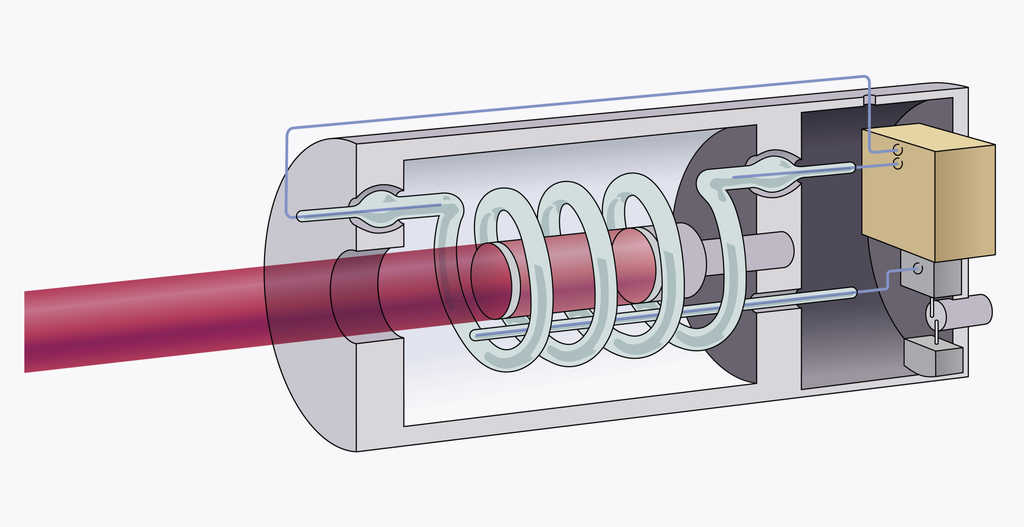
\includegraphics[width=0.6\textwidth]{Laserfysik/rubin_laser_diagram.jpg}
  \caption{Skematisk tegning af en rubin-laser}
  \label{fig:rubin_diagram}
\end{figure}
 Det er overgange i $\text{Cr}^{3+}$, som udsender laserens røde lys.
\opg Overvej, hvorfor lampen er formet som en spiral rundt om krystallen (se figur \ref{fig:rubin_diagram}).
\opg Figur \ref{fig:rubin_energi_diagram} viser de relevante energi-niveauer for $\text{Cr}^{3+}$. Fotonerne fra blitzlampen pumper atomerne op i de højere energiniveauer $E_3$ og $E_4$, som henfalder til to niveauer, som ligger meget tæt på hinanden, samlet kaldet $E_2$. Levetiden af $E_2$-niveauet er længere end levetiden af atomet i $E_3$ og $E_4$, så antallet at atomer i $E_2$ kan blive højere end i de andre niveauer, inklusiv grundtilstanden pga. pumpningen fra blitzlampen. Derfor kan der udsendes fotoner ved hjælp af stimuleret emission fra $E_2$, som udsendes med to røde bølgelængder (se Figur \ref{fig:rubin_energi_diagram}). 
\begin{figure}[h!]
  \centering
  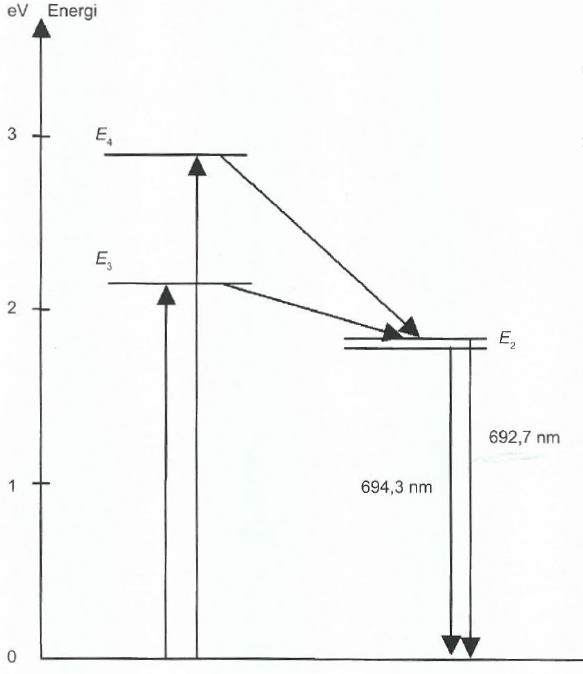
\includegraphics[width=0.5\textwidth]{Laserfysik/rubin_energi}
  \caption{De relevante energi-niveauer i $\text{Cr}^{3+}$.}
  \label{fig:rubin_energi_diagram}
\end{figure}
Hvilken energi bærer laserens udsendte fotoner (ca.)?

\emph{svar: $\approx 2,9\cdot 10^{-19} \joule$}
\opg En lasers rubinkrystal har form som en cylinder med længde $L=6\centi\meter$ og diameter $D=0,5\centi\meter$. I krystallen er $0,035\%$ af aluminiumatomerne udskiftet med $\text{Cr}^{3+}$. Hvor mange $\text{Cr}^{3+}$-atomer findes i krystallen? Du skal bruge følgende oplysninger: tætheden af aluminium er $\rho_\text{Al}=2,7\g/\cm^3$, den molære vægt af aluminium er $M_\text{Al}=27\g/\mol$ og man relaterer antallet af atomer per mol af et stof gennem Avogadros tal: $R_A = 6,022 \cdot 10^{23} \mol^{-1}$. \emph{Hint: find først antal aluminiumatomer indeholdt i cylinderens volumen}.

\emph{svar: $\approx 2,5 \cdot 10^{19}$} 
\opg En rubinlaser bliver ofte for varm til at udsende lys kontinuert, og udsender derfor i stedet lyset i pulser. Forestil dig, at alle $\text{Cr}^{3+}$-atomerne i laseren fra sidste delopgave (se svaret nederst i opgaven) er pumpet så de nu befinder sig i $E_2$, hvorefter laseren udsender alle fotoner med én puls med varighed $2,5 \cdot 10^{-6}\s$. Hvad er effekten af én laserpuls?
\opg En rubinlaser har ingen spejle, men krystallens ender er slebet for at kunne reflektere fotonerne og skabe stående bølger. Hvor mange hele antal bølgelængder svarer længden $L \approx 6\centi\meter$ af en rubinkrystal til for laserlys med $\lambda = 694,4 \cdot 10^{-9} \m$?. Hvor mange knudepunkter opstår i de stående bølger?
\opg Kan du forestille dig, hvorfor det er vigtigt at holde en laser ved stabil temperatur?
\end{opgave}

\begin{opgave}{Approksimation af Gevinstkoefficient}{2}
Denne opgave kræver brug af opgave 8 fra matematik opgaverne. \\
Såfremt reflektiviteten af spejlene i en laserkavitet er stor, dvs. $r_1r_2>0,9$ kan gevinstkoefficienten $g(\nu)$ (ligning 2.20) approksimeres til ligning 2.21. 
\opg Beregn hvordan ligning 2.20 approksimeres til ligning 2.21. \emph{Hint: antag $r_1r_2\approx 1-x$ og sæt $a=0$.}
\end{opgave}

\begin{opgave}{Flere--Niveau systemer}{2}
I Laserfysik er et 3-- og 4--niveau lasersystem præsenteret. Det gives at pumperaten ved tærskelværdien for systemerne er hhv. 
\begin{equation}
(P_t)_3 = \frac{N_T+\Delta N_t}{N_T - \Delta N_t}\Gamma_{21} \,\,\,\,\,\, \text{og} \,\,\,\,\,\, (P_t)_4 = \frac{\Delta N_t}{N_T - \Delta N_t}\Gamma_{21},
\end{equation}
hvor $N_T$ er den totale population og $\Delta N_t$ er $N_2-N_1$ ved tærskelværdien. 
\opg Hvilket system kræver mindst pumpning? Og hvorfor ser vi på pumperaterne ved tærskelværdien? 
\opg Hvilket system ville du foretrække? Hvorfor? 
\end{opgave}

\begin{opgave}{Kavitet}{1}
Et medium har en længde på 10 cm og en gevinstkoefficient på $0,025$cm$^-1$. To spejle med samme reflektivitet placeres i enderne af mediet. Vi antager at tabene ved spejlene pga. absorption og spredning er så små, at de kan negligeres. 
\opg Beregn reflektiviteten, der er nødvendig for at lasing kan opnåes. 
\opg Hvad er transmissionskoefficienten? 
\opg Er det optimalt at have to spejle med samme reflektivitet i en laser system? Hvorfor, hvorfor ikke?
\end{opgave}

\begin{opgave}{Foton Output}{2}
En kavitet for en He-Ne laser(632,8 nm) er 50 cm med reflektivitet $r_1=1$ for det ene spejl og $r_2=0,98$ for det andet spejl. Vi antager at tabene er meget små. Effekten (output power) af laseren er $Pwr = 10$ mW. 
\opg Hvor mange fotoner udsendes pr. sekund?
\opg Hvad er antallet af fotoner i kaviteten ved tærskelværdien?
\end{opgave}

\begin{opgave}{Pulserende eller Kontinuert?}{1}
En laser, der bruges til at skære i elementer, som f.eks. plastik har en væsentlig større intensitet end en laserpointer, der bruges i undervisningen (heldigvis!).
\opg Hvis du skulle bygge begge lasere, ville du så lave dem kontinuerte eller pulserende? Hvorfor?
\end{opgave}

\newpage


\chapter{Laserfysik Facitliste}

\begin{opgave}{Lasere med Forskellige Farver}{1}
\opg Atomerne har forskellige overgangsenergier. Bølgelængden afhænger af energien, og da rødt og grønt lys ikke har samme bølgelængde, må overgangsenergierne derfor være forskellige for atomerne, der bruges til at lave hhv. rødt og grønt lys. 
\opg Rød har længere bølgelængde end grøn, og grøn har derfor en større frekvens, da bølgelængde og frekvens er omvendt proportionale. 
\end{opgave}

\begin{opgave}{Partikel--Bølge--Dualitet}{2}
\opg Bølger kan intefere, som vi kender det fra stående bølger på en snor. De kan inteferere konstruktivt eller destruktivt. Ved konstruktiv inteferens vil man se en lysplet, da to bølger ''lægges sammen'', hvor i mod man ved destruktiv inteferens ikke vil se en lys plet, da bølgerne her vil udslukke hinanden. 
\opg Hvis lyset kun har partikelegenskaber kan man tænke på lys som små kugler, og man vil derfor forvente kun at se to lysprikker, der vil opstå pga. de to spalter i pladen. 
\end{opgave}

\begin{opgave}{Populationinversion}{2}
\opg Se på billedet for stimuleret emission. Vend nu processen om, dvs. Elektronen nu ligger i grundtilstanden. I denne omvendte proces kommer der altså to fotoner ind, hvoraf en af dem absorberes af elektronen, således at den hopper op i den exciterede tilstand. Den anden foton fortsætter bare og har ingen effekt. Hvis du nu sætter en ekstra foton ind i billedet for stimuleret absorption er det præcis det samme billede, som lige beskrevet som den omvendte proces af stimuleret emission. 
\opg Da vi nu har argumenteret for, at stimuleret emission og stimuleret absorption er de omvendte processer af hinanden, må de også ske med samme sandsynlighed.  Lige stor sandsynlighed for de to processer betyder at man kan sige at hver gang ét atom exciteres, så henfalder et andet atom. Derfor kan størstedelen af atomerne aldrig være i en exciteret tilstand, og stimuleret emission kan ikke dominere. Derfor kan 2-niveau-systemer ikke bruges til at skabe laserlys med.
\end{opgave}

\begin{opgave}{Verdens Første Laser -- Rubin Laseren}{3}
\opg Hvis lampen er formet rundt om kaviteten, så belyser den fra så mange retninger som muligt, hvilket effektivt kan pumpe systemet.
\opg På figuren ses det, at de udsendte fotoner har bølgelængderne $\lambda=692,7\nano\m$ og $\lambda=694,3\nano\m$ ($1\nano\m = 1$ nanometer $= 10^{-9}\m$). Vi tager gennemsnittet af de to for at udregne den gennemsnitlige energi af en foton.
\begin{align}
E_\text{foton} &= h \cdot \frac{c}{\lambda} \\
&= h \frac{c}{\left( 692,7 \cdot 10^{-9} \m + 694,3 \cdot 10^{-9} \m \right)/2} \\
&\approx 2,9 \cdot 10^{-19}\joule 
\end{align}
\opg Hvis man vil finde antal aluminium-atomer i en volumen skal man bruge:
\begin{equation}
\text{\# atomer} = (\rho_\text{Al} \cdot V)/M_\text{Al} \cdot R_A,
\end{equation}
($\rho_\text{Al} \cdot V$ giver antal gram aluminium i cylinderen, og deler man med den molare masse, så ved man hvor mange mol, der findes i cylinderen. Ved at gange med Avogadros tal, $R_A$, så finder man antal atomer). Volumenet af cylinderen er $V=\pi(D/2)^2 \cdot L$. Antal aluminium-atomer er derfor
\begin{equation}
\text{ \# Al-atomer} \approx 7 \cdot 10^{22}.
\end{equation}
Idet vi får at vide at $0,035\%$ af aluminium-atomerne er udskiftet med $\text{Cr}^{3+}$, så finder vi antal Cr-atomer som:
\begin{align}
\# \text{Cr-atomer} &= \#\text{Al-atomer} \cdot \frac{0,035}{100} \\
&\approx 2,5 \cdot 10^{19}.
\end{align}
\opg Effekten er udsendt energi per sekund. Hvis alle Cr-atomerne udsender lys på én gang, så er den samlede puls-energi $E_\text{puls} = E_\text{foton} \cdot \# \text{Cr-atomer}$, hvor vi bruger at vi fandt energien af en foton i delopgave 2. Effekten findes:
\begin{align}
P_\text{puls} &= \frac{E_\text{puls}}{t_\text{puls}} \\
&= \frac{ E_\text{foton} \cdot \# \text{Cr-atomer}}{t_\text{puls}} \\
&= \frac{2,9\cdot 10^{-19}\joule \cdot 2,5 \cdot 10^{19}}{2,5 \cdot 10^{-6}\s} \\
&= 2,9 \mega\watt
\end{align}
\opg For en krystal med længde $L=6\centi\meter$ og $\lambda = 694,4 \cdot 10^{-9} \m$ så er antal bølgelængder ca.
\begin{equation}
\frac{L}{\lambda} = 86406
\end{equation}
Vi ved at der opstår stående bølger i kaviteten, og at der derfor gælder:
\begin{align}
L &= n\frac{\lambda}{2} \\
\rightarrow n &= 2 \frac{L}{\lambda} \\
&= 172812 
\end{align}
Ved f.eks. at kigge på figur 4.3 så ses det, at antal knudepunkter er givet ved $n+1$. Antal knudepunkter er derfor $172813$.
\opg Hvis materialer opvarmes eller nedkøles vil de hhv. udvide og trække sig sammen, hvilket i værste fald kan resultere i, at længden af kaviteten ændres, sådan at der ikke kan opstå stående bølger.
\end{opgave}

\begin{opgave}{Approksimation af Gevinstkoefficient}{2}
\opg Ligningen der skal approksimeres er 
\begin{equation}
g_t = -\frac{1}{2L}\ln(r_1r_2). 
\end{equation}
Vi følger hintet og sætter $r_1r_2 = 1-x$, så 
\begin{equation}
g_t = -\frac{1}{2L}\ln(1-x). 
\end{equation}
Vi ønsker nu at approksimere funktionen med en Taylor udvikling. Vi sætter startsbetingelsen $a=0$ jævnfør hintet, og vi ser kun på de to første led. De andre led kan også beregnes, men de bidrager kun ganske lidt. 
\begin{equation}
f(x) \approx f(0) + x\d{f}{x}_{x=0} = 0 + x\cdot \frac{-1}{1-0} = -x
\end{equation}
$g_t$ bliver derfor 
\begin{equation}
g_t = -\frac{1}{2L}(-(1-r_1r_2)) = \frac{1}{2L}(1-r_1r_2). 
\end{equation}
\end{opgave}

\begin{opgave}{Flere-Niveau Systemer}{2}
\opg Vi ser på forholdet mellem dem for at finde ud af hvilket system, der kræver mindst pumpning. 
\begin{equation}
\frac{(P_t)_4}{(P_t)_3} = \frac{\Delta N_t}{N_T + \Delta N_t}.
\end{equation}
Det totale antal af atomer i systemet må være større end populationinversionen, så 
\begin{equation}
(P_t)_4 << (P_t)_3.
\end{equation}
For at opnå lasing kræver et 3 system mere pumpning end et 4 system. 
Vi ser på pumperaterne ved tærskelværdien fordi det lige akkurat er ved denne at lasing kan opnåes. 
\opg Med et 4 system kan vi opnå lasing med en lavere pumperate, og det er derfor at foretrække. 
\end{opgave}

\begin{opgave}{Kavitet}{1}
\opg Da man på forhånd ikke ved om spejlene opfylder $r_1r_2>0,9$ er det ikke gangbart at bruge den approksimerede version af $g_t$. Vi skal altså bruge 
\begin{equation}
g_t = -\frac{1}{2l}\ln(r_1r_2). 
\end{equation}
Da reflektiviteterne antages at være ens, kan vi sætte $r_1r_2=r^2$, som derefter isoleres. 
\begin{align}
g_t &= -\frac{1}{2l}\ln(r^2) 
\Rightarrow\\ -2lg_t &=\ln(r^2) 
\Rightarrow\\ e^{-2lg_t} &=r^2
\Rightarrow\\ r&=\sqrt{e^{-2lg_t}}
\end{align}
Indsættes tallene fås nu
\begin{equation}
r=\sqrt{e^{-2lg_t}} = \sqrt{e^{-2\cdot10\,\text{cm}\cdot0,025\,\text{cm}^{-1}}} = 0,778
\end{equation}
\opg Da $s$ antages at være 0 gælder der $r+t=1$. Transmissionskoefficienten fås da til 
\begin{equation}
r+t=1 \Rightarrow t = 1-r = 1-0,778 = 0,222. 
\end{equation}
Det vil altså sige, at $77,8\%$ af lyset reflekteres og $22,2\%$ transmitteres når lyset rammer et af spejlene. 
\opg Det er ikke optimalt at have to spejle med samme reflektivitet da man kun ønsker, at laserlyset skal komme ud i den ene ende. Derudover kan man heller opnå at $r_1r_2>0,9$ hvis begge reflektviteter er mindre end 1. 
\end{opgave}

\begin{opgave}{Foton Output}{2}
\opg Vi får givet effekten (power) af laserlyset. Effekt har enheden watt, som er defineret som energi pr. tid, dvs. $\text{W} = \frac{\text{J}}{\text{s}}$. Fra dette kan vi se, at det er nødvendigt at dividere med en energi for at få noget pr. sekund. Altså er antallet af udsendte fotoner pr. sekund 
\begin{equation}
\d{q}{t} = \frac{\text{Pwr}}{h\nu},
\end{equation}
hvor $h\nu$ er energien af én foton
\begin{equation}
h\nu = h \frac{c}{\lambda} = 6,626\cdot 10^{-34}\, \text{Js} \, \frac{3\cdot10^{8}\,\text{m/s}}{632,8\cdot 10^{-9}\, \text{m}} = 3,14\cdot 10^{-19}\, \text{J}.
\end{equation}
Vi får så at 
\begin{equation}
\d{q}{t} = \frac{10\cdot10^{-3}\,\text{W}}{3,14\cdot 10^{-19}\,\text{J}} = 3,14\cdot 10^{-16}\, \frac{1}{\text{s}}.
\end{equation}
\opg Vi bruger at 
\begin{equation}
\d{q}{t} = cg(\nu)q, 
\end{equation}
og da vi skal beregen antallet af fotoner ved tærskelværdien er $g(\nu) = g_t$. Vi får da 
\begin{equation}
q = \d{q}{t}\frac{1}{cg_t} = \frac{\text{Pwr}}{h\nu}\frac{1}{cg_t}.
\end{equation}
Da $r_1r_2>0,9$ kan $g_t$ beregnes til 
\begin{equation}
g_t = \frac{1}{2\cdot 0,5 \, \text{m}}(1-0,98) = 0,02\, \text{m}^{-1}. 
\end{equation}
Antallet af fotoner bliver så 
\begin{equation}
q = 3,14\cdot 10^{-16}\, \frac{1}{\text{s}}\, \frac{1}{3\cdot 10^{8} \text{m/s}\cdot 0,02 \, \text{m}^{-1}} = 5,2\cdot 10^9
\end{equation}
\end{opgave}

\begin{opgave}{Pulserende eller Kontinuert}{1}
\opg En pulserende laser pumpes oftest hårdere fordi det kræver mere at opnå populationinversion pga. alle tabene. En kontinuert laser pumpes ikke nær så hårdt da lasersystemet ikke lider af så store tab, som en pulserende laser gør. En større pumpning giver anledning til mere stimuleret emission, der så giver anledning til mere intenst lys. Intensiteten af en pulserende laser er derfor typisk større, da et sådant lasersystem pumpes hårdere. 
\end{opgave}



%Når du starter på en opgave skriver du \begin{opgave}{navnet på opgaven}{sværhedsgrad}, hvor sværhedsgraden skrives som 1,2 eller 3, hvor 3 er den sværeste. 
%Når opgaven er slut skrives \end{opgave}. 
%Såfremt der er delopgaver skrives delopgaver som \opg 

%Eksempel på opgave 
%\begin{opgave}{Polære koordinater}{1}
  %Den kinetiske energi af et legeme, der bevæger sig i 2D-planet er
  %i kartesiske koordinater ($x$ og $y$) givet ved ligning
  %(1.11).
  %
  %\opg Beregn $\dt{x}$ og $\dt{y}$ i polære koordinater og vis
  %derefter, at den kinetiske energi udtrykt i polære koordinater er
  %givet ved ligning (1.12).
%\end{opgave}

\chapter{Relativitetsteori Opgaver}

\begin{opgave}{Det Galileiske Relativitetsprincip}{1}
Det Galileiske Relativitetsprincip siger, at Newtons bevægelseslove er ens i alle inertielle referencesystemer.\\
Vi forestiller os nu et tog, der kører med en konstant hastighed $v$ ift. sporet. En passager i toget tager så en sten og slipper den fra hvile.  
\opg Brug Galileis relativitetsprincip til at beskrive stenens bevægelse set fra en observatør i toget.
\opg Brug Galilei-transformationen (3.1) til at give en beskrivelse af stenens bevægelse set fra en observatør på Jorden. 
\end{opgave}

\begin{opgave}{Kombination af Galileiske transformationer}{1}	
	To tog kører parallelt med hinanden i $x$-retningen, det ene med hastighed $V$ og det andet med hastighed $U$,
	relativt til jorden. Lad det første tog være $S'$ og det andet $S''$, med deres respektive koordinater. Jorden betegnes $S$.
	\opg Hvad er den Galileiske transformation fra $S \left( x,y,z,t \right)$ til $S'' \left( x'',y'',z'',t'' \right)$?
	\opg Hvad er den Galileiske transformation fra $S'$ til $S''$?
	\opg Hvad svarer størrelsen $\left( U- V \right)$ til?	 
\end{opgave}

\begin{opgave}{Løbetur i Regnvejr}{1}
En dag hvor det regner, falder dråberne ned med $\SI{2}{m/s}$. En person løber vandret af sted med $\SI{3}{m/s}$. Ved hvilken vinkel ift. vandret skal personen holde sin paraply for bedst muligt at skærme for regnen? (hint: Kig på regndråbernes bevægelse set fra løberens referencesystem).
\end{opgave}

\begin{opgave}{Flyvetur i Blæsevejr}{1}
En flyvemaskine kan flyve med  $\SI{500}{km/t}$, og der er en vindhastighed på $\SI{200}{km/t}$ fra vest mod øst.
\opg Flyets pilot styrer flyet mod nord. I hvilken retning bevæger flyet sig, og hvad er flyets hastighed set fra en observatør på Jorden, som betegnes $S$? (hint: Kig på et referencesystem $S'$, der bevæger sig med vinden og benyt hastighedstransformationerne (3.2) til at oversætte flyets bevægelse i dette system til $S$).
\opg I hvilken retning skal piloten styre, hvis flyet skal flyve mod nord? Hvad er flyets hastighed set fra en observatør på Jorden i dette tilfælde?
\end{opgave}

\begin{opgave}{Flodræset}{2}
En flod er $\SI{20}{m}$ bred og vandet i floden strømmer af sted med en hastighed på $\SI{1}{m/s}$. To svømmere Arthur og Barbara arrangerer et ræs. Arthur skal svømme $\SI{20}{m}$ ned af floden og tilbage, mens Barbara skal svømme lige over floden og tilbage. Både Arthur og Barbare kan svømme med $\SI{2}{m/s}$.
\opg I hvilken retning skal Barbara svømme, for at hun kommer lige over floden?
\opg Hvem vinder ræset og med hvor meget?
\end{opgave}

\begin{opgave}{Hvornår er relativitetsteori virkelig nødvendig?}{1}
	Som det ses, så indgår $\gamma$ meget ofte i relativitetsteori. Når $\gamma$ er væsentligt større end 1, er det
	nødvendigt at bruge de relativistiske udtryk, frem for de Galileiske. For hvilken hastighed (i enheder af $c$) er
	værdien af $\gamma$:
	\opg 1\% større end 1?
	\opg 10\% større end 1?
	\opg 100\% større end 1?
\end{opgave}

\begin{opgave}{Et lille tankeeksperiment}{1}
	De relativistiske effekter ses ikke i hverdagen, fordi $c$ er så stor, sammenlignet med hastigheder vi oplever i
	hverdagen. Men hvad nu hvis lysets hastighed var meget mindre? Lad os se hvad der sker, hvis nu $c = 50\,\kilo\meter$/t.
	\opg Usain Bolts topfart er $\SI{44,72}{km/t}$. Hans hvilemasse er $94 \si{kg}$. Hvad er hans masse, når han når
	topfart?
\end{opgave}

\begin{opgave}{Muoner i Jordens atmosfære}{1}
	Muoner er ustabile sub-atomare partikler, der med en levetid på $2,2 \,\mu\si{\s}$ $(2,2 \cdot 10^{-6} \si{s})$ henfalder til elektroner.
	Muoner produceres omkring $10 \si{km}$ over Jordens overflade, hvor energirige partikler fra rummet rammer
	atmosfæren, og de rejser med en hastighed tæt på lysets i forhold til Jorden, lad os sige $v = 0,999c$.
	\opg Hvad er den længste afstand en muon kan nå at rejse i sin levetid på $2,2 \,\mu\si{\s}$?
	\opg Fra ovenstående lader det til, at muonerne aldrig vil nå os på overfladen. Ikke desto mindre detekterer vi
	dem! Men levetiden angivet er i muonens hvilesystem. Hvad er dens levetid målt for en observatør på
	Jorden?
	\opg Hvor langt vil muonen nå nu?
	\opg Fra muonens synspunkt lever den stadig kun $2,2 \, \mu\si{\s}$. Hvad er tykkelsen af $10 \si{km}$ atmosfære, set fra
	muonens system?
\end{opgave}

\begin{opgave}{Relativitet og rumfart}{1}
	For nyligt valgte NASA at pensionere deres rumfærger. Indtil da var rumfærgen en forholdsvis billig måde at
	fragte udstyr og mennesker ud i rummet, fordi færgen og det meste af det man brugte til at sende den op med
	kunne genanvendes. Efter endt mission kunne rumfærgen lande som et fly.\\
	\indent
	En observatør på Jorden måler en landingsbane til at være $3600 \si{m}$. En rumfærge befinder sig i kredsløb om
	Jorden med en hastighed af $4,00 \cdot 10^7 \si{m/s}$ relativt til Jorden. Vi antager, at dens bane er en ret linje under hele
	opgaven, og at den flyver parallelt med landingsbanen.
	\opg Hvad er længden af landingsbanen målt af piloten på rumfærgen?
	\opg En observatør på Jorden måler tiden der går, fra rumfærgen er direkte over den ene ende af landingsbanen,
	og til den er over den anden ende. Hvor lang tid får vedkommende?
	\opg Piloten på rumfærgen måler den tid, det tager ham at flyve længden af landingsbanen. Hvilken værdi får
	han?
	\opg Rumfærgen har en vægt på godt $2000$ tons. Hvad ville rumfærgen veje, hvis en observatør på Jorden
	kunne veje den, mens den var i kredsløb, dvs. hvad er dens relativistiske masse?
	\opg Rumfærgen er $60$ meter lang og $10$ meter høj i dens eget referencesystem. Hvor lang og høj er rumfærgen
	for en observatør på Jorden?
\end{opgave}

\begin{opgave}{Tvillinge-Paradokset - Her skal du bruge hovedet}{2}
	Tvillinge-paradokset er et af de mest kendte paradokser inden for speciel relativitetsteori. Egentligt er det ikke
	et paradoks, da Einstein allerede løste det tilbage i 1905. I denne opgave skal I også løse det. Det kræver, at man
	lige tænker sig lidt om.
	
	Barbara og Arthur er tvillinger. Arthur bliver på Jorden, mens Barbara rejser af sted med et rumskib, med
	hastighed nær $c$. På et tidspunkt vender rumskibet hurtigt, og flyver tilbage til Jorden. Da Barbara kommer
	tilbage, mødes hun med Arthur til en sammenligning. For Arthur har Barbara rejst ud og hjem igen med nær
	lysets hastighed. Derfor er tiden for hende gået langsommere, og hun vil derfor se yngre ud end Arthur. Men
	fra Barbaras synspunkt er det jo Arthur, som har bevæget sig i forhold til hende. Derfor bruger hun samme
	argument til at konkludere, at han vil se yngre ud end hende. Samtidigt er der jo ikke noget referencesystem,
	som er bedre end andre, så et argument der bygger på dette vil komme frem til, at alle resultater må være
	symmetriske mellem de to tvillinger. De er altså lige gamle.
	\opg Ud fra ovenstående lader det til, at der er tre muligheder, men kun en kan være rigtig. Hvilken mulighed
	er det?
	\opg Hvis en af tvillingerne er ældst, kan du så sige noget om, hvor lang tid der er gået for den yngste i
	forhold til den ældste?
\end{opgave}


\begin{opgave}{Lorentz-transformationens udledelse}{2}
	I afsnit 3.7 udledte vi Lorentz-transformationen. I ligning 3.15 så vi på højresiden, hvor vi konkluderede at $x$'s koefficient skulle være 1, og herved fandt frem til gamma-funktionen $\gamma$. Vi var dog ikke helt færdig med udledelsen i dette tilfælde.
	\opg I skal nu færdiggøre udledelsen af Lorentz-transformationen, ved at undersøge om højresiden af ligning 3.15 stemmer overens med ligning 3.11, når vi kender $\gamma$.
\end{opgave}

\begin{opgave}{Lorentz-transformationen på differens-form}{2}
	\label{lorentz_diff}
	Lad os betragte to begivenheder $P_1$ og $P_2$, som i inertialsystemet $S$ har koordinaterne $(x_1,y_1,z_1,t_1)$ og $(x_2,y_2,z_2,t_2)$. Svarende hertil har vi de fire koordinatdifferencer
	\begin{align}
		\Delta t=t_2-t_1, \	 \Delta x=x_2-x_1, \ \Delta y=y_2-y_1, \ \Delta z= z_2-z_1 \nonumber
	\end{align}
	\opg I skal nu finde de tilsvarende størrelser,
	\begin{math}
		\Delta t',  \Delta x',  \Delta y',  \Delta z'
	\end{math}
	i inertialsystemet $S'$, som bevæger sig i forhold til $S$ med hastigheden $v$, ved hjælp af Lorentz-transformationen.
\end{opgave}

\begin{opgave}{Tidsforlængelse og Længdeforkortelse vha. Lorenz-transformationen}{2}
	I denne opgave skal I prøve at udlede formlen for tidsforlængelse og længdeforkortelse vha. Lorentz-transformationen. Det gøres ved at kigge på en proces set fra to referencesystemer $S$ og $S'$ i standardkonfigurationen. Processens start og slutning i tid og rum beskrives ved $(x_1,t_1)$ og $(x_2,t_2)$ i $S$ og $(x'_1,t'_1)$ og $(x'_2,t'_2)$ i $S'$.
	\opg Udtrykket for $\Delta t'$ I fandt i opgave \ref{lorentz_diff} indeholder både $t_1,t_2$ og $x_1,x_2$. Hvad må man kræve omkring processens start-- og slutkoordinater $x_1$ og $x_2$ i $S$, for at udtrykket bliver lig udtrykket for tidsforlængelse?
	\opg Forklar hvorfor kravet fra 1) sikre, at vi kigger på en "ren" tidsforlængelse, hvor rum og tid ikke bliver blandet sammen.
	\opg Forklar hvordan udtrykket for $\Delta t'$ fra opgave \ref{lorentz_diff}, hvis man ikke bruger kravet fra 1), viser at rum og tid bliver blandet sammen i relativitetsteori.
	\opg Gennemgå de samme trin som I har gjort ovenfor, denne gang hvor I kigger på længdeforkortelse. Start derfor med $\Delta x'$, og undersøg hvad man må kræve omkring $t_1$ og $t_2$.
\end{opgave}

\begin{opgave}{Cæsars død og Kristi fødsel}{2}
	Cæsar blev myrdet år 44 f.Kr., og afstanden fra Rom til Betlehem kan sættes til 2300 km.
	\opg Findes der nogen iagttager, for hvem Cæsars død og Kristi fødsel er samtidige? Hvorfor/hvorfor ikke?
\end{opgave}

\begin{opgave}{Samtidighed}{2}
	To begivenheder har i inertialsystemet $S$ koordinaterne $(t_1,x_1,y_1,z_1)=(L/c,L,0,0)$ og $(t_2,x_2,y_2,z_2)=(L/2c,2L,0,0)$.
	\opg Der findes et inertialsystem, $S'$, i hvilket disse begivenheder er samtidige. Find hastigheden af $S'$ i forhold til $S$.
	\opg Hvad er den fælles tidskoordinat, $t'$, for disse begivenheder i $S'$?
\end{opgave}

\begin{opgave}{En stangs hastighed}{2}
	En stang med hvilelængde $l_0$ bevæger sig med jævn hastighed i sin længderetning. Set fra $S$ tager det tiden $\tau$ for stangen at passere et fast punkt i $S$. 
	\opg Find stangens hastighed som en brøkdel af lysets hastighed, $c$.
\end{opgave}

\begin{opgave}{Invarians af lyspuls bevægelse}{2}
	Et referencesystem $S'$ bevæger sig i $x$-retningen med hastigheden $v$ relativt til et andet referencesystem $S$. Til tiden $t'=t=0$ krydser de to referencesystemer hinanden (deres origo er samme sted), og i netop dette øjeblik udsendes en lyspuls fra origo i $S'$. Efter en tid $t'$ er lyspulsens afstand $x'$ i $S'$ givet ved $x'^2 = c^2 t'^2$. 
	\opg Vis at afstanden $x$ i $S$ er givet ved $x^2 = c^2 t^2$ (hint: Brug Lorentz transformationerne). 
\end{opgave}

\begin{opgave}{Referencesystemer - samme sted og samme tid}{3}
	To begivenheder er observeret i et referencesystem $S$ og kan beskrives ved $\left( x_1 , t_1 \right)$ og $\left( x_2 , t_2 \right)$. Et andet referencesystem $S'$ bevæger sig langs $x$-aksen med en hastighed $v$, således at de to begivenheder sker samme sted på $x$-aksen set fra $S'$.
	\opg Vis at tidsforskellen $\Delta t'$ mellem begivenhederne i $S'$ er givet ved:
	$$\Delta t' = \sqrt{\left( \Delta t \right)^2 - \left( \frac{\Delta x}{c} \right)^2}$$
	(hint: Brug $x'_1 = x'_2$ og Lorentz-transformationerne).
	\opg Brug ovenstående resultat til at vise, at såfremt $\Delta x > c \Delta t$, så vil der ikke eksistere et referencesystem $S'$, hvor begivenhederne sker samme sted.
	\opg Hvis $\Delta x > c \Delta t$, så findes der i stedet et andet referencesystem $S'$, hvor de to begivenheder sker samtidigt. Vis at afstanden $\Delta x'$ mellem de to begivenheder i dette referencesystem er givet ved:
	$$\Delta x' = \sqrt{\left( \Delta x \right)^2 - c^2 \left( \Delta t \right)^2}$$
	(hint: Brug $t'_1 = t'_2$ og Lorentz-transformationerne).
	\opg Brug ovenstående resultat til at vise, at såfremt $c \Delta t > \Delta x$, så vil der ikke eksistere et referencesystem $S'$, hvor begivenhederne sker samtidigt.
\end{opgave}


I de følgende to opgaver, vil det være nødvendigt at kigge på funktioner af to variable, og hvordan sådanne funktioner ændre sig, når begge variable ændre sig på samme tid. 
Forestil jer, at  vi har en funktion $z$, der afhænger både af $y$ og $x$. Dette skriver man typisk $z=f \left( x,y \right)$. Hvis man har en ændring $\Delta x$ samt en ændring $\Delta y$ kan man approksimere ændringen $\Delta z$ på følgende måde:

$$\Delta z \approx \d{z}{x} \cdot \Delta x + \d{z}{y} \cdot \Delta y$$


Såfremt man lader ændringerne $\Delta x$ og $\Delta y$ gå mod nul, vil ovenstående ikke længere være en approksimation, og man skriver at:

$$dz = \d{z}{x} \cdot dx + \d{z}{y} \cdot dy$$


hvor $dz$, $dy$ og $dx$ er infinitesimale (meget små) versioner af $\Delta z$, $\Delta y$ og $\Delta x$.\\

\begin{opgave}{Lorentz-transformationen for hastighed}{2}
	I denne opgave skal i prøve at udlede Lorentz-transformationen for hastighed. Dette kan gøres ved at finde et udtryk for $dx'$ og $dt'$, som det er beskrevet ovenfor. Da $dx'$ og $dt'$ vil være de øjeblikkelige ændringer i $x'$ og $t'$, må det derfor gælde at $v'_x = dx'/dt'$.
\end{opgave}

\begin{opgave}{Lorentz-transformationen for acceleration}{3}
	Lad $S'$ være et referencesystem der bevæger sig med hastighed $v$ i forhold til et andet referencesystem $S$. Et objekt bevæger sig relativt i forhold til $S$ langs $x$-aksen med en øjeblikkelig hastighed $v_x$ og øjeblikkelig acceleration $a_x$. Målet med de følgende trin er at finde et udtryk for accelerationen $a'_x$ i referencesystemet $S'$.
	\opg Find et udtryk for $dt'$.
	\opg Find et udtryk for $dv'_x$.
	
	
	Før det sidste trin er det værd at sikre jer, at i har fået de rigtige resultater. I skulle gerne have fundet at:
	$$dt' = \gamma \left( dt - v dx / c^2 \right)$$
	$$dv'_x = \left( \frac{1 - v^2/c^2}{ \left( 1-vv_x/c^2 \right)^2 } \right) dv_x$$
	\opg Brug at $a'_x = dv'_x / dt'$, $a_x = dx/dt$ samt at $v_x = dx/dt$ til at vise, at $a'_x$ er givet ved:
	$$a'_x = a_x \left( 1- \frac{v^2}{c^2} \right)^{3/2} \left( 1 - \frac{vv_x}{c^2}  \right)^{-3}$$
\end{opgave}

\begin{opgave}{Relativitet og Newtons 2. lov}{3}
	I denne opgave skal i bruge den relativistiske impuls, $\kraft{p}{rel}$, og den nye definition af Newtons 2. lov, $F = \d{p}{t}$, til at vise udtrykket for den relativistiske kraft $\kraft{F}{rel}$. I skal altså sætte ind og regne jer frem til resultatet.
\end{opgave}

\chapter{Relativitetsteori Facitliste}

\begin{opgave}{Det Galileiske Relativitetsprincip}{1}
	Det Galileiske Relativitetsprincip siger, at Newtons bevægelseslove er ens i alle inertielle referencesystemer.\\
	Vi forestiller os nu et tog, der kører med en konstant hastighed $v$ ift. sporet. En passager i toget tager så en sten og slipper den fra hvile.  
	\opg Brug Galileis relativitetsprincip til at beskrive stenens bevægelse set fra en observatør i toget.\\
	
	Da toget bevæger sig med konstant hastighed, er det et inertialsystem. Vi ved, at en sted falder lodret ned mod jorden i et inertialsystem, der er i hvile, og derfor må den også gøre det i toget. Newtons bevægelseslove er jo ens i alle inertialesystemer.\\  
	\opg Brug Galilei-transformationen (3.1) til at give en beskrivelse af stenens bevægelse set fra en observatør på Jorden.\\
	
	Lad $x$-aksen pege i den retning, som toget kører. Da stenen falder lodret nedad i toget, vil $x'=0$ for alle tider $t$ og $t'$. Fra Galilei-transformationen for $x'$ får man da at:
	
	$$0 = x-vt \quad \Rightarrow \quad x = vt$$
	
	Stenen falder altså ikke lodret ned set fra Jorden, da den har fået en vertikal hastighed på $v$. 
\end{opgave}

\begin{opgave}{Kombination af Galileiske transformationer}{1}	
	To tog kører parallelt med hinanden i $x$-retningen, det ene med hastighed $V$ og det andet med hastighed $U$,
	relativt til jorden. Lad det første tog være $S'$ og det andet $S''$, med deres respektive koordinater. Jorden betegnes $S$.
	\opg Hvad er den Galileiske transformation fra $S \left( x,y,z,t \right)$ til $S'' \left( x'',y'',z'',t'' \right)$?\\
	
	Her bruger man formlerne for de Galileiske transformationer (3.1). Man får at:
	
	$$t''=t$$
	$$x''=x-Ut$$
	$$y''=y$$
	$$z''=z$$
	\opg Hvad er den Galileiske transformation fra $S'$ til $S''$?\\

	Her bruger man formlerne for de Galileiske transformationer (3.1). Man får at:
	
	$$t''=t'$$
	$$y''=y'$$
	$$z''=z'$$
	
	For at finde transformationen for $x''$, kan man først finde transformationen for $x'$. Den er fra (3.1): $x' = x - Vt $. Så kan man løse for $x$, hvilket giver: $x = x' + Vt$. Dette kan man så indsætte i udtrykket for $x''$, hvor man får:
	
	$$x'' = x-Ut = x' + Vt -Ut = x' - \left( U - V \right)t = x' - \left( U-V \right)t'$$
	
	hvor det er brugt at $t=t'$.\\
	\opg Hvad svarer størrelsen $\left( U- V \right)$ til?\\
	

	$U-V$ er $S''$ systemets hastighed relativt til $S'$ systemet.	 
\end{opgave}

\begin{opgave}{Løbetur i Regnvejr}{1}
	En dag hvor det regner, falder dråberne lodret ned med $\SI{2}{m/s}$. En person løber vandret af sted med $\SI{3}{m/s}$. Ved hvilken vinkel ift. vandret skal personen holde sin paraply for bedst muligt at skærme for regnen? (hint: Kig på regndråbernes bevægelse set fra løberens referencesystem).\\
	
	Set fra løberens referencesystem falder regnen ikke lodret ned, da det har både en lodret hastighed ($\SI{2}{m/s}$) og en vandret hastighed ($\SI{3}{m/s}$). Kigger man på dråbens fald over $\SI{1}{s}$, vil dråben bevæge sig langs hypotenusen i en trekanten nedenfor:
	\begin{center}
	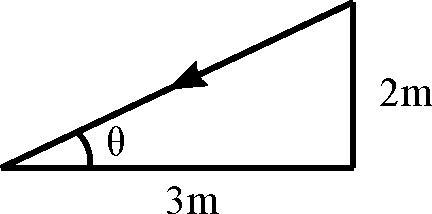
\includegraphics[scale=0.9]{Relativitetsteori/regn_fig.pdf}	
	\end{center}
	
	Man finder da $\theta$:
	
	$$\theta = \arctan \left( \frac{2}{3} \right) = 33.69^\circ$$	
\end{opgave}

\begin{opgave}{Flyvetur i Blæsevejr}{1}
	En flyvemaskine kan flyve med  $\SI{500}{km/t}$, og der er en vindhastighed på $\SI{200}{km/t}$ fra vest mod øst.
	\opg Flyets pilot styrer flyet mod nord. I hvilken retning bevæger flyet sig, og hvad er flyets hastighed set fra en observatør på Jorden, som betegnes $S$? (hint: Kig på et referencesystem $S'$, der bevæger sig med vinden og benyt hastighedstransformationerne (3.2) til at oversætte flyets bevægelse i dette system til $S$).\\
	
	Lad $y$-aksen pege mod nord og $x$-aksen pege mod øst. Lad videre $x$- og $x'$-aksen være parallelle, og de to systemers origoer være sammenfaldende for $t=t'=0$. Kigger man på flyet fra $S'$, vil der ikke være nogen vind. Derfor flyver flyet direkte nord på set fra dette system. Det må betyde, at flyets hastigheder i de forskellige retninger er:
	
	$$u'_y = \SI{500}{km/t} \quad \quad \text{og} \quad \quad u'_x = u'_z = 0$$
	
	\vspace{2mm}
	
	Kigger man på (3.2) får man da at $u_y = u'_y$ og $u_z = u'_z$. For $u_x$ får man:
	
	$$u'_x = 0 = u_x - v \quad \Rightarrow \quad u_x = v = \SI{200}{km/t}$$
	
	\vspace{2mm}
	
	da $v$ jo er vindens hastighed her. For at finde den retning som flyet flyver i, set fra Jorden, kan man kigge på flyets bevægelse over 1 time:
	
	\begin{center}
		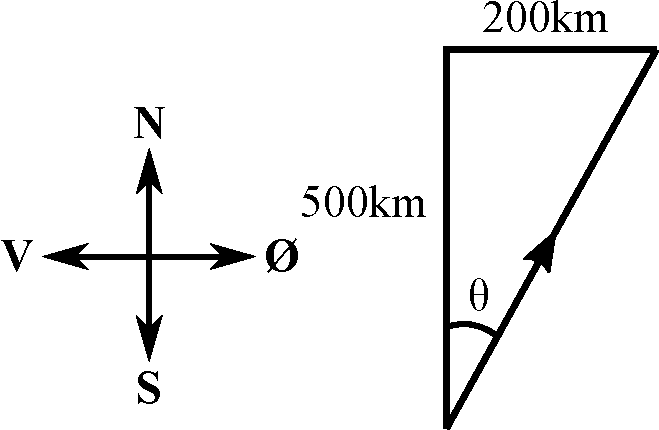
\includegraphics[scale=0.8]{Relativitetsteori/fly_fig.pdf}
	\end{center}
	
	Så findes $\theta$:
	
	$$\theta = \arctan \left( \frac{200}{500} \right) = 21.80^\circ$$
	
	\vspace{2mm}
	
	Og Flyets hastighed set fra Jorden findes vha. Pythagoras:
	
	$$v_{\text{fly}} = \sqrt{500^2 + 200^2} \, \si{km/t} = \SI{538.52}{km/t} $$
	\opg I hvilken retning skal piloten styre, hvis flyet skal flyve mod nord? Hvad er flyets hastighed set fra en observatør på Jorden i dette tilfælde?\\
	
	Hvis flyet skal flyve mod nord, er det nødt til at have en hastighed $u_x = - \SI{200}{km/t}$. Igen får man en trekant:
	
	\begin{center}
		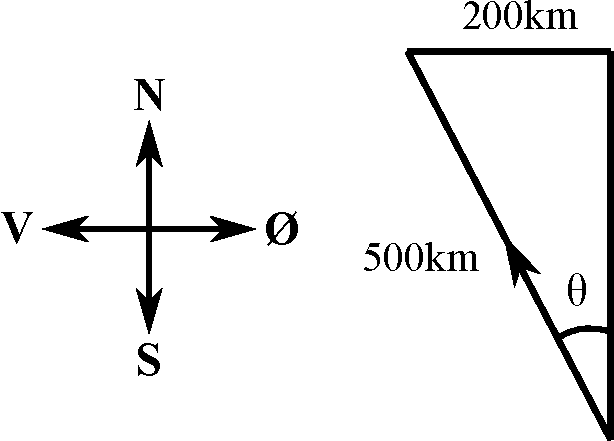
\includegraphics[scale=0.8]{Relativitetsteori/fly_fig2.pdf}
	\end{center}

	Man kan finde $\theta$:
	
	$$\sin \theta = \frac{\SI{200}{km}}{\SI{500}{km}} \quad \Rightarrow \quad \theta = \arcsin \left( \frac{200}{500} \right) = 23.58^\circ$$
	
	Og hastigheden bliver:
	
	$$v_{\text{fly}} = \sqrt{500^2 - 200^2} \ \si{km/t} = \SI{458.26}{km / t}$$
\end{opgave}

\begin{opgave}{Flodræset}{2}
	En flod er $\SI{20}{m}$ bred og vandet i floden strømmer af sted med en hastighed på $\SI{1}{m/s}$. To svømmere Arthur og Barbara arrangerer et ræs. Arthur skal svømme $\SI{20}{m}$ ned af floden og tilbage, mens Barbara skal svømme lige over floden og tilbage. Både Arthur og Barbare kan svømme med $\SI{2}{m/s}$.
	\opg I hvilken retning skal Barbara svømme, for at hun kommer lige over floden?\\
	
	Set fra et referencesystem der bevæger sig med strømmen, skal Barbaras hastighed opad være $\SI{1}{m/s}$ og hendes totale hastighed $\SI{2}{m/s}$. Man kan lave en trekant, og finde at Barbara skal svømme med en vinkel $\theta$ ift. en lige linje over floden. Vinklen er:
	
	$$\theta = \arcsin \left( \frac{1}{2} \right) = 30.0^\circ$$
	\opg Hvem vinder ræset og med hvor meget?\\
	
	Kald bredten af floden for $L$. Barbara er praktisk talt nød til at svømme en længere tur. Længden hun svømmer hver vej er givet:
	
	$$\cos \theta = \frac{L}{L_{\text{Bar}}} \quad \quad \Rightarrow \quad \quad L_{\text{Bar}} = \frac{L}{\cos \theta}  $$
	
	\vspace{2mm}
	
	For Barbara tager hele turen altså:
	
	$$t_{\text{Bar}} = \frac{2 \cdot L_{\text{Bar}}}{\SI{2}{m/s}} = \frac{2 \cdot \SI{20}{m}}{\cos \left( 30.0^\circ \right) \cdot \SI{2}{m/s}} = \SI{23.09}{s}$$
	
	\vspace{2mm}
	
	For Arthur kan man regne tiden for hver af de to ture:
	
	$$t_{\text{Art,ned}} = \frac{\SI{20}{m}}{\SI{3}{m/s}} = \SI{6.667}{s}$$
	
	$$t_{\text{Art,op}} = \frac{\SI{20}{m}}{\SI{1}{m/s}} = \SI{20}{s}$$
	
	\vspace{2mm}
	
	Det giver:
	
	$$t_{\text{Art}} = t_{\text{Art,ned}} + t_{\text{Art,op}} = \SI{26.667}{s}$$
	
	\vspace{2mm}
	
	Barbara vinder altså ræset.
\end{opgave}


\begin{opgave}{Hvornår er relativitetsteori virkelig nødvendig?}{1}
	Som det ses, så indgår $\gamma$ meget ofte i relativitetsteori. Når $\gamma$ væsentligt større end 1, er det
	nødvendigt at bruge de relativistiske udtryk, frem for de Galileiske. For hvilken hastighed (i enheder af $c$) er
	værdien af $\gamma$:
	\opg 1\% større end 1?
	\opg 10\% større end 1?
	\opg 100\% større end 1?\\
	
	Her kan man opskrive følgende:
	
	$$x = \frac{1}{\sqrt{1- v^2/c^2}} \quad \Rightarrow \quad \frac{v}{c} = \sqrt{1- \frac{1}{x^2}}$$
	
	
	\noindent
	Så kan man ellers bare indsætte $1.01$, $1.10$ og $2.00$ på $x$'s plads, hvorved man finder at:
	
	$$\gamma = 1.01 \quad \Rightarrow \quad \frac{v}{c} = 0.1404 $$
	$$\gamma = 1.10 \quad \Rightarrow \quad \frac{v}{c} = 0.4166 $$
	$$\gamma = 2 \quad \Rightarrow \quad \frac{v}{c} = 0.8660 $$
\end{opgave}

\begin{opgave}{Et lille tankeeksperiment}{1}
	De relativistiske effekter ses ikke i hverdagen, fordi $c$ er så stor, sammenlignet med hastigheder vi oplever i
	hverdagen. Men hvad nu hvis lysets hastighed var meget mindre? Lad os se hvad der sker, hvis nu $c = 50$
	km/t.
	\opg Usain Bolts topfart er $44,72 \si{km/t}$. Hans hvilemasse er $94 \si{kg}$. Hvad er hans masse, når han når
	topfart?\\
	
	Her bruger man (3.25), der giver den relativistiske masse. Det giver at:
	
	$$m_{\text{rel}} = \frac{\SI{94}{kg}}{\sqrt{1- (\SI{44.72}{km/t})^2 / (\SI{50}{km/t})^2}} =  \SI{210.2}{kg} $$
\end{opgave}

\begin{opgave}{Muoner i Jordens atmosfære}{1}
	Muoner er ustabile sub-atomare partikler, der med en levetid på $2,2 \,\mu\si{\s}$ $(2,2 \cdot 10^{-6} \si{s})$ henfalder til elektroner.
	Muoner produceres omkring $10 \si{km}$ over Jordens overflade, hvor energirige partikler fra rummet rammer
	atmosfæren, og de rejser med en hastighed tæt på lysets i forhold til Jorden, lad os sige $v = 0,999c$.
	\opg Hvad er den længste afstand en muon kan nå at rejse i sin levetid på $2,2 \,\mu\si{\s}$?\\
	
	Den er givet som:
	
	$$L = v \cdot T_0 = 0.999 \cdot 3.00 \times 10^8 \ \si{m/s} \cdot 2.2 \times 10^{-6} \ \si{s} = \SI{659.34}{m}$$
	\opg Fra ovenstående lader det til, at muonerne aldrig vil nå os på overfladen. Ikke desto mindre detekterer vi
	dem! Men levetiden angivet er i muonens hvilesystem. Hvad er dens levetid målt for en observatør på
	Jorden?\\
	
	Levetiden som målt af en observatør på Jorden er givet ved:
	
	$$T=\gamma T_0=\frac{2.2 \times 10^{-6}\si{s}}{\sqrt{1-0.999^2}}=49.2058 \times 10^{-6}\si{s}=49.2058\mu\si{s} $$
	\opg Hvor langt vil muonen nå nu?\\
	
	Mounen når nu en længde på 
	$$L=v \cdot T=0.999 \cdot 3.00 \times 10^8 \si{m/s} \cdot 49.2058 \times 10^{-6} = 14746.98 \si{m} = 14.74698 \si{km}$$
	\opg Fra muonens synspunkt lever den stadig kun $2,2 \, \mu\si{\s}$. Hvad er tykkelsen af $10 \si{km}$ atmosfære, set fra
	muonens system?\\
	
	Set fra mounens system, vil atmosfæren have en tykkelse på
	$$L=\frac{L_0}{\gamma}=10000 \si{m} \cdot \sqrt{1-0.999^2} = 447.102 \ \si{m}$$
\end{opgave}

\begin{opgave}{Relativitet og rumfart}{1}
	For nyligt valgte NASA at pensionere deres rumfærger. Indtil da var rumfærgen en forholdsvis billig måde at
	fragte udstyr og mennesker ud i rummet, fordi færgen og det meste af det man brugte til at sende den op med
	kunne genanvendes. Efter endt mission kunne rumfærgen lande som et fly.\\
	\indent
	En observatør på Jorden måler en landingsbane til at være $3600 \si{m}$. En rumfærge befinder sig i kredsløb om
	Jorden med en hastighed af $4,00 \cdot 10^7 \si{m/s}$ relativt til Jorden. Vi antager, at dens bane er en ret linje under hele
	opgaven, og at den flyver parallelt med landingsbanen.
	\opg Hvad er længden af landingsbanen målt af piloten på rumfærgen?\\
	
	Længden af landingsbanen som målt af piloten er
	$$L=\frac{L_0}{\gamma}=3600 \si{m} \cdot \sqrt{1-\frac{16.00 \times 10^{14} \si{m/s}}{9.00 \times 10^{16} \si{m/s}}} = 3567.86 \si{m}$$
	\opg En observatør på Jorden måler tiden der går, fra rumfærgen er direkte over den ene ende af landingsbanen,
	og til den er over den anden ende. Hvor lang tid får vedkommende?\\
	
	Tiden er givet ved strækning divideret med hastigheden,
	$$t=\frac{3600 \si{m}}{4.00 \times 10^7 \si{m/s}} = 9 \times 10^{-5} \si{s}$$
	\opg Piloten på rumfærgen måler den tid, det tager ham at flyve længden af landingsbanen. Hvilken værdi får
	han?\\
	
	Denne opgave kan løses på to måder. Vi kan enten benytte os af den forkortede længde og bruge samme metode som tidligere,
	$$t=\frac{3567.86 \si{m}}{4.00 \times 10^7 \si{m/s}}=89.1965 \cdot 10^{-6} \si{s}$$
	
	Alternativt kan man udregne tiden ved at benytte sig af længdeforkortelse, hvor tiden målt fra rumfærgen er $T_0$,
	$$T_0=\frac{T}{\gamma}=9 \times 10^{-5} \si{s} \cdot \sqrt{1-\frac{16.00 \times 10^{14} \si{m/s}}{9.00 \times 10^{16} \si{m/s}}}=89.1965 \cdot 10^{-6} \si{s}$$
	\opg Rumfærgen har en vægt på godt $2000$ tons. Hvad ville rumfærgen veje, hvis en observatør på Jorden
	kunne veje den, mens den var i kredsløb, dvs. hvad er dens relativistiske masse?\\
	
	Rumfærgens relativistiske masse er givet ved
	$$m_{\text{rel}}=\gamma m=\frac{2.00 \times 10^6}{\sqrt{1-\frac{16.00 \times 10^{14} \si{m/s}}{9.00 \times 10^{16} \si{m/s}}}}=2.018 \times 10^6 \si{kg}$$
	\opg Rumfærgen er $60$ meter lang og $10$ meter høj i dens eget referencesystem. Hvor lang og høj er rumfærgen
	for en observatør på Jorden?\\
	
	Højden vil ikke ændre sig, da længdeforkortelse kun har en effekt i bevægelsesretningen. Længden som målt af en observatør på Jorden er
	$$L=\frac{L_0}{\gamma}=60 \si{m} \cdot \sqrt{1-\frac{16.00 \times 10^{14} \si{m/s}}{9.00 \times 10^{16} \si{m/s}}}=49.464 \si{m}$$
\end{opgave}

\begin{opgave}{Tvillinge-Paradokset - Her skal du bruge hovedet}{2}
	Tvillinge-paradokset er et af de mest kendte paradokser inden for speciel relativitetsteori. Egentligt er det ikke
	et paradoks, da Einstein allerede løste det tilbage i 1905. I denne opgave skal I også løse det. Det kræver, at man
	lige tænker sig lidt om.
	
	Barbara og Arthur er tvillinger. Arthur bliver på Jorden, mens Barbara rejser af sted med et rumskib, med
	hastighed nær $c$. På et tidspunkt vender rumskibet hurtigt, og flyver tilbage til Jorden. Da Barbara kommer
	tilbage, mødes hun med Arthur til en sammenligning. For Arthur har Barbara rejst ud og hjem igen med nær
	lysets hastighed. Derfor er tiden for hende gået langsommere, og hun vil derfor se yngre ud end Arthur. Men
	fra Barbaras synspunkt er det jo Arthur, som har bevæget sig i forhold til hende. Derfor bruger hun samme
	argument til at konkludere, at han vil se yngre ud end hende. Samtidigt er der jo ikke noget referencesystem,
	som er bedre end andre, så et argument der bygger på dette vil komme frem til, at alle resultater må være
	symmetriske mellem de to tvillinger. De er altså lige gamle.
	\opg Ud fra ovenstående lader det til, at der er tre muligheder, men kun en kan være rigtig. Hvilken mulighed
	er det?\\
	
	Svaret ligger i at Barbaras rumskib bliver nød til at accelerere, når det vender for at flyve tilbage til jorden. Barbaras referencesystem vil altså ikke være et inertielt referencesystem, og den specielle relativitetsteori, vil derfor ikke gælde for hende. Det betyder således at problemet ikke er symmetrisk set fra de to tvillinger, og det rigtige svar er derfor, at Barbara er yngre end Arthur.\\
	\opg Hvis en af tvillingerne er ældst, kan du så sige noget om, hvor lang tid der er gået for den yngste i
	forhold til den ældste?\\
	
	Tiden der er gået for den ældste tvilling er $T$. Vi kan så bruge formlen for tidsforlængelse til at finde den tid der er gået for den yngste,
	$$T_0=T \cdot \sqrt{1-\frac{v^2}{c^2}}$$
\end{opgave}


\begin{opgave}{Lorentz-transformationens udledelse}{2}
	I afsnit 3.7 udledte vi Lorentz-transformationen. I ligning 3.15 så vi på højresiden, hvor vi konkluderede at $x$'s koefficient skulle være 1, og herved fandt frem til gamma-funktionen $\gamma$. Vi var dog ikke helt færdig med udledelsen i dette tilfælde.
	\opg I skal nu færdiggøre udledelsen af Lorentz-transformationen, ved at undersøge om højresiden af ligning 3.15 stemmer overens med ligning 3.11, når vi kender $\gamma$.\\
	
	Vi søger i denne opgave at omskrive højresiden af 3.15, $c^2\gamma^2t^2-\gamma^2v^2t^2$, ved hjælp af $\gamma$ funktionen, således at det stemmer overens med højresiden af 3.11, $c^2t^2$.
	\begin{align*}
		&c^2\gamma^2t^2-\gamma^2v^2t^2 \\
		&\downarrow \\
		&c^2t^2\gamma^2(1-v^2/c^2) \\
		&\downarrow \\
		&c^2t^2\frac{1}{1-v^2/c^2} \\
		&\downarrow \\
		&c^2t^2
	\end{align*}
\end{opgave}

\begin{opgave}{Lorentz-transformationen på differens-form}{2} \label{lorentz_diff2}
	Lad os betragte to begivenheder $P_1$ og $P_2$, som i inertialsystemet $S$ har koordinaterne $(x_1,y_1,z_1,t_1)$ og $(x_2,y_2,z_2,t_2)$. Svarende hertil har vi de fire koordinatdifferencer
	\begin{align}
		\Delta t=t_2-t_1, \	 \Delta x=x_2-x_1, \ \Delta y=y_2-y_1, \ \Delta z= z_2-z_1 \nonumber
	\end{align}
	\opg I skal nu finde de tilsvarende størrelser,
	\begin{math}
		\Delta t',  \Delta x',  \Delta y',  \Delta z'
	\end{math}
	i inertialsystemet $S'$, som bevæger sig i forhold til $S$ med hastigheden $v$, ved hjælp af Lorentz-transformationen.\\
	
	Da vi har $\Delta t=t_2-t_1$, må den tilsvarende differens i $S'$ være $\Delta t'=t'_2-t'_1$. Vi kan herved finde et udtryk for denne differens ved at bruge Lorentz-transformationen,
	\begin{align*}
		\Delta t'=\gamma(t_2-vx_2/c^2)-\gamma(t_1-vx_1/c^2)=\gamma(t_2-t_1-vx_2/c^2+vx_1/c^2)=\gamma(\Delta t-v\Delta x/c^2)
	\end{align*}
	Man gør det samme for de tre andre størrelser:
	$$\Delta x' = \gamma \left( x_2 - vt_2 \right) - \gamma \left( x_1 - vt_1 \right) = \gamma \left( x_2 - x_1 -vt_2 + vt_1 \right) = \gamma \left( \Delta x - v \Delta t \right)$$
	
	$$\Delta y' = y'_2 - y'_1 = y_2 - y_1 = \Delta y \quad \quad \text{og} \quad \quad \Delta z' = z'_2 - z'_1 = z_2 - z_1 = \Delta z$$
\end{opgave}

\begin{opgave}{Tidsforlængelse og Længdeforkortelse vha. Lorenz-transformationen}{2}
	I denne opgave skal I prøve at udlede formlen for tidsforlængelse og længdeforkortelse vha. Lorentz-transformationen. Det gøres ved at kigge på en proces set fra to referencesystemer $S$ og $S'$ i standardkonfigurationen. Processens start og slutning i tid og rum beskrives ved $(x_1,t_1)$ og $(x_2,t_2)$ i $S$ og $(x'_1,t'_1)$ og $(x'_2,t'_2)$ i $S'$.
	\opg Udtrykket for $\Delta t'$ I fandt i opgave \ref{lorentz_diff2} indeholder både $t_1,t_2$ og $x_1,x_2$. Hvad må man kræve omkring processens start-- og slutkoordinater $x_1$ og $x_2$ i $S$, for at udtrykket bliver lig udtrykket for tidsforlængelse?\\
	
	Man må kræve at $x_1=x_2$, således at man har $\Delta t'=\gamma(\Delta t-v \cdot 0/c^2)=\gamma\Delta t$.\\
	\opg Forklar hvorfor kravet fra 1) sikre, at vi kigger på en "ren" tidsforlængelse, hvor rum og tid ikke bliver blandet sammen.\\
	
	I tilfældet af at $\Delta t' =\gamma\Delta t$, kan vi se at tiden $\Delta t'$ kun afhænger af den relative hastighed og tidsforskellen $\Delta t$ i $S$. Hvis vi ikke krævede at $\Delta x=0$, ville udtrykket afhænge både af de forrige variable og begivenhedernes position.\\
	\opg Forklar hvordan udtrykket for $\Delta t'$ fra opgave \ref{lorentz_diff2}, hvis man ikke bruger kravet fra 1), viser at rum og tid bliver blandet sammen i relativitetsteori.\\
	
	Se opgave 13.2.\\
	\opg Gennemgå de samme trin som I har gjort ovenfor, denne gang hvor I kigger på længdeforkortelse. Start derfor med $\Delta x'$, og undersøg hvad man må kræve omkring $t_1$ og $t_2$.\\
	
	I dette tilfælde vil $\Delta x'$ være hvilelængden. For at udtrykket for $\Delta x'$ skal stemme overens med udtrykket for længdeforkortelse, må vi kræve at $t_1=t_2$, således at vi har
	\begin{align*}
	&\Delta x'=\gamma(\Delta x-v*0) \\
	&\downarrow \\
	&\Delta x=\frac{\Delta x'}{\gamma}
	\end{align*}
	
	Vi ser her igen at kravet om at $\Delta t = 0$ resulterer i en "ren" længdeforkortelse, da udtrykket kun afhænger af den relative hastighed $v$ og hvilelængden $\Delta x'$.
\end{opgave}

\begin{opgave}{Cæsars død og Kristi fødsel}{2}
	Cæsar blev myrdet år 44 f.Kr., og afstanden fra Rom til Betlehem kan sættes til 2300 km.
	\opg Findes der nogen iagttager, for hvem Cæsars død og Kristi fødsel er samtidige? Hvorfor/hvorfor ikke?\\
	
	Vi skal i denne opgave bruge den tidslige Lorentz-transformationen på differensform. Man kan så opstille to inertialsystemer $S$ og $S'$, hvor $S'$ bevæger sig med hastigheden $v$ i forhold til $S$. For at de to begivenheder sker samtidigt skal $\Delta t'=0$, og man kan herved opstille en ligning og isolere den nødvendige hastighed $v$.
	\begin{align*}
		&0=\gamma(\Delta t-v\Delta x/c^2) \\
		&\downarrow \\
		&0=\frac{\Delta t-v\Delta x/c^2}{\sqrt{1-v^2/c^2}} \\
		&\downarrow \\
		&0=\Delta t-v\Delta x/c^2 \\
		&\downarrow \\
		&\frac{\Delta tc^2}{\Delta x}=v
	\end{align*}
	Vi indsætter de opgivet størrelser og udregner hastigheden,
	\begin{align*}
		v=\frac{1387584000 s \cdot (3.00\cdot 10^8)}{2300000 m}=5.430 \times 10^{19}  \ \si{m/s}
	\end{align*}
	Vi kan herved konkludere at der ikke findes nogen iagttager, for hvem Cæsars død og Kristi fødsel er samtidige, da den nødvendige hastighed er langt større end lysets hastighed.
\end{opgave}

\begin{opgave}{Samtidighed}{2}
	To begivenheder har i inertialsystemet $S$ koordinaterne $(t_1,x_1,y_1,z_1)=(L/c,L,0,0)$ og $(t_2,x_2,y_2,z_2)=(L/2c,2L,0,0)$.
	\opg Der findes et inertialsystem, $S'$, i hvilket disse begivenheder er samtidige. Find hastigheden af $S'$ i forhold til $S$.\\
	
	I denne opgave skal vi benytte os af det samme udtryk som vi kom frem til i den forrige opgave. Denne gang er $\Delta t=\frac{L}{2c}-\frac{L}{c}=\frac{Lc}{2c^2}-\frac{Lc}{c^2}=-\frac{L}{2c}$ og $\Delta x=2L-L=L$. Dette indsættes, og et udtryk for hastigheden udregnes,
	\begin{align*}
		v=-\frac{\frac{L}{2c}c^2}{L}=-\frac{\frac{Lc}{2}}{L}=-\frac{Lc}{2L}=-\frac{c}{2}
	\end{align*}
	\opg Hvad er den fælles tidskoordinat, $t'$, for disse begivenheder i $S'$?\\
	
	Da vi nu kender hastigheden $v$, kan vi finde et udtryk for den fælles tidskoordinat $t'$ for de to begivenheder ved at bruge den tidslige Lorentz-transformation,
	\begin{align*}
		&t'=\gamma(\frac{L}{c}+\frac{cL}{2c^2}) \\
		&\downarrow \\
		&t'=\gamma(\frac{2L}{2c}+\frac{L}{2c}) \\
		&\downarrow \\
		&t'=\gamma\frac{3L}{2c} \\
		&\downarrow \\
		&t'=\sqrt{\frac{4}{3}}\frac{3}{2}\frac{L}{c} \\
		&\downarrow \\
		&t'=\sqrt{\frac{4}{3}}\sqrt{\frac{9}{4}}\frac{L}{c} \\
		&\downarrow \\
		&t'=\sqrt{3}\frac{L}{c}
	\end{align*}
\end{opgave}

\begin{opgave}{En stangs hastighed}{2}
	En stang med hvilelængde $l_0$ bevæger sig med jævn hastighed i sin længderetning. Set fra $S$ tager det tiden $\tau$ for stangen at passere et fast punkt i $S$. 
	\opg Find stangens hastighed som en brøkdel af lysets hastighed, $c$?\\
	
	Ved brug af længdeforkortnings formlen, er stangens længde i $S$ givet ved $L=L_0\sqrt{1-v^2/c^2}$. Herudover kan vi beskrive længden i $S$ ved $L=v\tau$. Vi kan herved bruge disse to udtryk til at finde stangens hastighed,
	\begin{align*}
		&v\tau=L_0\sqrt{(1-v^2/c^2)} \\
		&\downarrow \\
		&v^2\tau^2=L_0^2(1-v^2/c^2) \\
		&\downarrow \\
		&v^2\frac{\tau^2}{L_0^2}=1-v^2/c^2 \\
		&\downarrow \\
		&\frac{v^2}{c^2}(\frac{\tau^2}{L_0^2}+1)=1 \\
		&\downarrow \\
		&\frac{v}{c}=\frac{1}{\sqrt{\frac{\tau^2}{L_0^2}+1}}
	\end{align*}
\end{opgave}

\begin{opgave}{Invarians af lyspuls bevægelse}{2}
	Et referencesystem $S'$ bevæger sig i $x$-retningen med hastigheden $v$ relativt til et andet referencesystem $S$. Til tiden $t'=t=0$ krydser de to referencesystemer hinanden (deres origo er samme sted), og i netop dette øjeblik udsendes en lyspuls fra origo i $S'$. Efter en tid $t'$ er lyspulsens afstand $x'$ i $S'$ givet ved $x'^2 = c^2 t'^2$. 
	\opg Vis at afstanden $x$ i $S$ er givet ved $x^2 = c^2 t^2$ (hint: Brug Lorentz transformationerne).\\
	
		Vi benytter os her af den Lorentz-transformationen for $t'$ og $x'$:
	\begin{align*}
	&\gamma^2(x-vt)^2=c^2\gamma^2(t-vx/c^2)^2 \\
	&\downarrow \\
	&x-vt=c \cdot (t-vx/c^2) \\
	&\downarrow \\
	&x+vx/c=ct+vt \\
	&\downarrow \\
	&x(1+v/c)=ct(1+v/c) \\
	&\downarrow \\
	&x=ct \\
	&\downarrow \\
	&x^2=c^2t^2		
	\end{align*} 
\end{opgave}

\begin{opgave}{Referencesystemer - samme sted og samme tid}{3}
	To begivenheder er observeret i et referencesystem $S$ og kan beskrives ved $\left( x_1 , t_1 \right)$ og $\left( x_2 , t_2 \right)$. Et andet referencesystem $S'$ bevæger sig langs $x$-aksen med en hastighed $v$, således at de to begivenheder sker samme sted på $x$-aksen set fra $S'$.
	\opg Vis at tidsforskellen $\Delta t'$ mellem begivenhederne i $S'$ er givet ved:
	$$\Delta t' = \sqrt{\left( \Delta t \right)^2 - \left( \frac{\Delta x}{c} \right)^2}$$
	(hint: Brug $x'_1 = x'_2$ og Lorentz-transformationerne).\\
	
	$t_1'=t_2'$ og Lorentz-transformationen bruges først til at opstille et udtryk for hastigheden $v$,
	\begin{align*}
	&x_1-vt_1=x_2-vt_2 \\
	&\downarrow \\
	&\Delta x=v \cdot \Delta t \\
	&\downarrow \\
	&v=\frac{\Delta x}{\Delta t} \\
	\end{align*}
	
	Herefter bruger vi Lorentz-transformationen på $\Delta t'=t_2'-t_1'$,
	\begin{align*}
	&\Delta t'=\gamma(t_2-vx_2/c^2)-\gamma(t_1-vx_1/c^2) \\
	&\downarrow \\
	&\Delta t'=\frac{\Delta t-\frac{v\Delta x}{c^2}}{\sqrt{1-\frac{v^2}{c^2}}} \\
	&\downarrow \\
	&\Delta t'=\frac{\Delta t - \frac{\Delta x^2}{\Delta t^2c^2}}{\sqrt{1-\frac{\Delta x^2}{\Delta t^2c^2}}}
	&\downarrow \\
	&\Delta t'=\frac{\Delta t - \frac{\Delta x^2}{\Delta t^2c^2}}{\sqrt{1-\frac{\Delta x^2}{\Delta t^2c^2}}} \cdot \frac{\sqrt{\Delta t^2}}{\sqrt{\Delta t^2}} \\
	&\downarrow \\
	&\Delta t'=\frac{\Delta t^2-\frac{\Delta x^2}{c^2}}{\sqrt{\Delta t^2-\frac{\Delta x^2}{c^2}}} \\
	&\downarrow \\
	&\Delta t' = \sqrt{\Delta t^2-\frac{\Delta x^2}{c^2}}
	\end{align*}
	\opg Brug ovenstående resultat til at vise, at såfremt $\Delta x > c \Delta t$, så vil der ikke eksistere et referencesystem $S'$, hvor begivenhederne sker samme sted.\\
	
	Vi indser først at $\Delta x^2 > c^2\Delta t^2$ er det samme som $\Delta x > c\Delta t$. Vi kan så omskrive det forrige udtryk til
	$$\Delta t'=\sqrt{\frac{c^2\Delta t^2-\Delta x^2}{c^2}}$$
	Hvis $\Delta x^2 > c^2\Delta t^2$ er gældende, vil $\Delta t'$ være imaginært. Medmindre du er Stephen Hawking, så er imaginær tid udefineret.\\
	\opg Hvis $\Delta x > c \Delta t$, så findes der i stedet et andet referencesystem $S'$, hvor de to begivenheder sker samtidigt. Vis at afstanden $\Delta x'$ mellem de to begivenheder i dette referencesystem er givet ved:
	$$\Delta x' = \sqrt{\left( \Delta x \right)^2 - c^2 \left( \Delta t \right)^2}$$
	(hint: Brug $t'_1 = t'_2$ og Lorentz-transformationerne).\\
	
	$t_1'=t_2'$ benyttes til at udregne hastigheden $v$,
	\begin{align*}
	&t_1-x_1v/c^2=t_2-x_2v/c^2 \\
	&\downarrow \\
	&\Delta t=\frac{\Delta x v}{c^2} \\
	&\downarrow \\
	&v=\frac{c^2\Delta t}{\Delta x}
	\end{align*}
	Herefter bruger vi Lorentz-transformationen på $\Delta x'= x_2'-x_1'$,
	\begin{align*}
	&\Delta x'=\gamma(\Delta x-v\Delta t)=\frac{\Delta x-v\Delta t}{\sqrt{1-\frac{v^2}{c^2}}} \\
	&\downarrow \\
	&\Delta x'=\frac{\Delta x-\frac{c^2\Delta t^2}{\Delta x}}{\sqrt{1-\frac{c^2\Delta t^2}{\Delta x^2}}} \\
	&\downarrow \\
	&\Delta x'=\frac{\Delta x-\frac{c^2\Delta t^2}{\Delta x}}{\sqrt{1-\frac{c^2\Delta t^2}{\Delta x^2}}} \cdot \frac{\sqrt{\Delta x^2}}{\sqrt{\Delta x^2}} \\
	&\Delta x'=\frac{\Delta x^2-c^2\Delta t^2}{\sqrt{\Delta x^2-c^2\Delta t^2}} = \sqrt{\Delta x^2-c^2\Delta t^2}
	\end{align*}
	\opg Brug ovenstående resultat til at vise, at såfremt $c \Delta t > \Delta x$, så vil der ikke eksistere et referencesystem $S'$, hvor begivenhederne sker samtidigt.\\
	
		Ligesom i 18.2, så er $c^2\Delta t^2 > \Delta x^2$ ækvivalent med $c\Delta t > \Delta x$. I tilfældet af at $c^2\Delta t^2 > \Delta x^2$ er gældende, vil $\Delta x'$ ikke være reel.
\end{opgave}


I de følgende to opgaver, vil det være nødvendigt at kigge på funktioner af to variable, og hvordan sådanne funktioner ændre sig, når begge variable ændre sig på samme tid. 
Forestil jer, at  vi har en funktion $z$, der afhænger både af $y$ og $x$. Dette skriver man typisk $z=f \left( x,y \right)$. Hvis man har en ændring $\Delta x$ samt en ændring $\Delta y$ kan man approksimere ændringen $\Delta z$ på følgende måde:

$$\Delta z \approx \d{z}{x} \cdot \Delta x + \d{z}{y} \cdot \Delta y$$


Såfremt man lader ændringerne $\Delta x$ og $\Delta y$ gå mod nul, vil ovenstående ikke længere være en approksimation, og man skriver at:

$$dz = \d{z}{x} \cdot dx + \d{z}{y} \cdot dy$$


hvor $dz$, $dy$ og $dx$ er infinitesimale (meget små) versioner af $\Delta z$, $\Delta y$ og $\Delta x$.\\

\begin{opgave}{Lorentz-transformationen for hastighed}{2}
	I denne opgave skal i prøve at udlede Lorentz-transformationen for hastighed. Dette kan gøres ved at finde et udtryk for $dx'$ og $dt'$, som det er beskrevet ovenfor. Da $dx'$ og $dt'$ vil være de øjeblikkelige ændringer i $x'$ og $t'$, må det derfor gælde at $v'_x = dx'/dt'$.\\
	
	Som det første bruger man at:
	
	$$dx' = \d{x'}{x} \cdot dx + \d{x'}{t} \cdot dt = \frac{dx - v dt}{\sqrt{1- v^2 / c^2}} $$
	
	$$dt' = \d{t'}{x} \cdot dx + \d{t'}{t} \cdot dt = \frac{dt - v dx/c^2}{\sqrt{1- v^2 / c^2}}  $$
	
	Så finder man $v'_x$ ved at dividere disse:
	
	$$v'_x = dx'/dt' = \frac{\gamma (dx - v dt)}{\gamma (dt - v dx/c^2)} = \frac{dx - v dt}{dt - v dx/c^2} = \frac{dx/dt - v}{1 - v dx/dtc^2} = \frac{v_x - v}{1 - v v_x / c^2} $$
\end{opgave}

\begin{opgave}{Lorentz-transformationen for acceleration}{3}
	Lad $S'$ være et referencesystem der bevæger sig med hastighed $v$ i forhold til et andet referencesystem $S$. Et objekt bevæger sig relativt i forhold til $S$ langs $x$-aksen med en øjeblikkelig hastighed $v_x$ og øjeblikkelig acceleration $a_x$. Målet med de følgende trin er at finde et udtryk for accelerationen $a'_x$ i referencesystemet $S'$.
	\opg Find et udtryk for $dt'$.\\
	
	Dette findes som i forrige opgave.
	
	$$dt' = \d{t'}{x} \cdot dx + \d{t'}{t} \cdot dt = \frac{dt - v dx/c^2}{\sqrt{1- v^2 / c^2}}  $$
	\opg Find et udtryk for $dv'_x$.\\
	
	Da $v'_x$ kun afhænger af en variabel $v_x$ finder man at:
	
	$$dv'_x = \d{v'_x}{v_x} \cdot dv_x = \left( \d{\left( v_x - v \right)}{v_x}  \cdot \frac{1}{1-vv_x/c^2} + \d{\frac{1}{1-vv_x/c^2}}{v_x} \cdot (v_x-v) \right) dv_x  $$
	
	$$=  \left( \frac{1}{1-vv_x/c^2} + \frac{vv_x/c^2 - v^2/c^2}{\left( 1-vv_x/c^2 \right)^2} \right) dv_x = \left( \frac{1-vv_x/c^2}{\left( 1-vv_x/c^2 \right)^2} + \frac{vv_x/c^2 - v^2/c^2}{\left( 1-vv_x/c^2 \right)^2} \right) dv_x $$
	
	$$= \left( \frac{1-v^2/c^2}{\left( 1 - vv_x/c^2 \right)^2} \right) dv_x$$
	
	Før det sidste trin er det værd at sikre jer, at i har fået de rigtige resultater. I skulle gerne have fundet at:
	$$dt' = \gamma \left( dt - v dx / c^2 \right)$$
	$$dv'_x = \left( \frac{1 - v^2/c^2}{ \left( 1-vv_x/c^2 \right)^2 } \right) dv_x$$
	\opg Brug at $a'_x = dv'_x / dt'$, $a_x = dx/dt$ samt at $v_x = dx/dt$ til at vise, at $a'_x$ er givet ved:
	$$a'_x = a_x \left( 1- \frac{v^2}{c^2} \right)^{3/2}  \left( 1 - \frac{vv_x}{c^2}  \right)^{-3}$$
	
	Her dividerer man de to udtryk med hinanden.
	
	$$ a'_x = dv'_x/dt' = dv_x \frac{ (1 - v^2/c^2)/ \left( 1-vv_x/c^2 \right)^2}{\gamma \left( dt - v dx / c^2 \right)} = \frac{dv_x}{dt} \frac{ (1 - v^2/c^2)/ \left( 1-vv_x/c^2 \right)^2}{\gamma \left( 1 - v dx /dt c^2 \right)} $$
	
	$$ = a_x \frac{ (1 - v^2/c^2)/ \left( 1-vv_x/c^2 \right)^2}{\gamma \left( 1 - v v_x/ c^2 \right)} = a_x \left( 1- \frac{v^2}{c^2} \right)^{3/2} \left( 1 - \frac{vv_x}{c^2}  \right)^{-3}  $$
\end{opgave}

\begin{opgave}{Relativitet og Newtons 2. lov}{3}
	I denne opgave skal i bruge den relativistiske impuls, $\kraft{p}{rel}$, og den nye definition af Newtons 2. lov, $F = \d{p}{t}$, til at vise udtrykket for den relativistiske kraft $\kraft{F}{rel}$. I skal altså sætte ind og regne jer frem til resultatet.\\
	
	Dette findes ved følgende beregning:
	
	$$F = \d{p}{t} = \d{\frac{mv}{\sqrt{1-v^2/c^2}}}{t} = \d{mv}{t} \cdot \frac{1}{\sqrt{1-v^2/c^2}} + \d{\frac{1}{\sqrt{1-v^2/c^2}}}{t} \cdot mv  $$
	
	$$= \frac{ma}{\sqrt{1-v^2/c^2}} + \frac{mav^2/c^2}{\left( 1-v^2/c^2 \right)^{3/2}} = \frac{ma \left( 1 - v^2/c^2 \right)}{\left( 1-v^2/c^2 \right)^{3/2}} + \frac{mav^2/c^2}{\left( 1-v^2/c^2 \right)^{3/2}} = \frac{ma}{\left( 1-v^2/c^2 \right)^{3/2}} $$
\end{opgave}


\chapter{Rotationel Mekanik Udledning}
Her beskrives et fysisk pendul med masse $m$ og inertimoment $I$, hvor friktion ikke negligeres, og slutteligt vises det, hvad visse simplificeringer resulterer i. Det er tiltænkt at deltagerne selv laver kraftanalysen og beslutter hvilke kræfter, de antager pendulet er påvirket af, selvom snoren bør antages masseløs. Fremgangsmåden er den samme, så alle specialtilfælde beskrives ikke i detajler her. \\

\begin{figure}[]
\centering
\begin{subfigure}{.5\textwidth}
  \centering
  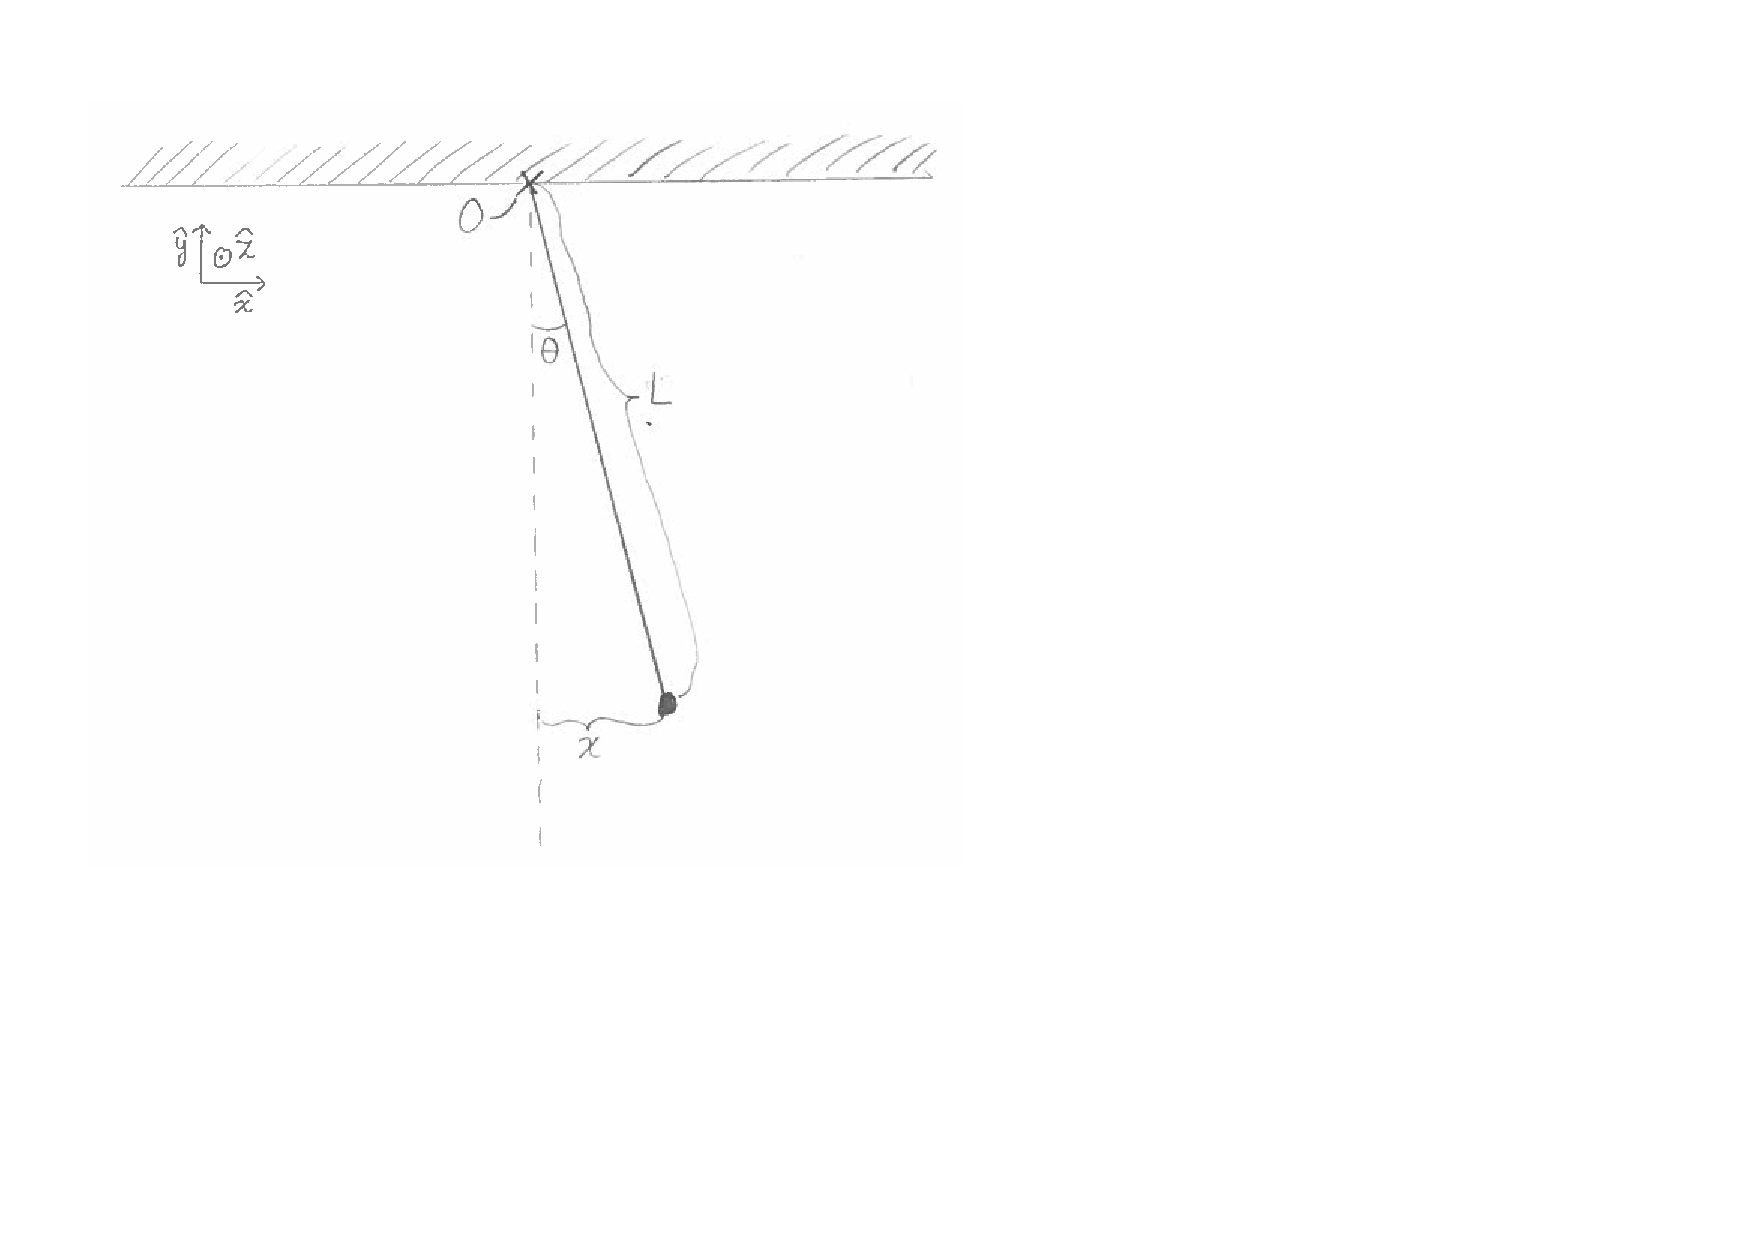
\includegraphics[width=\linewidth]{RotationelMekanik/Pendul}
\caption{Pendul med enhedsvektorer og stedvektor indtegnet til et arbitrært tidspunkt.}
\label{fig:Pendul}
\end{subfigure}
\hspace{5mm}
\begin{subfigure}{.45\textwidth}
  \centering
  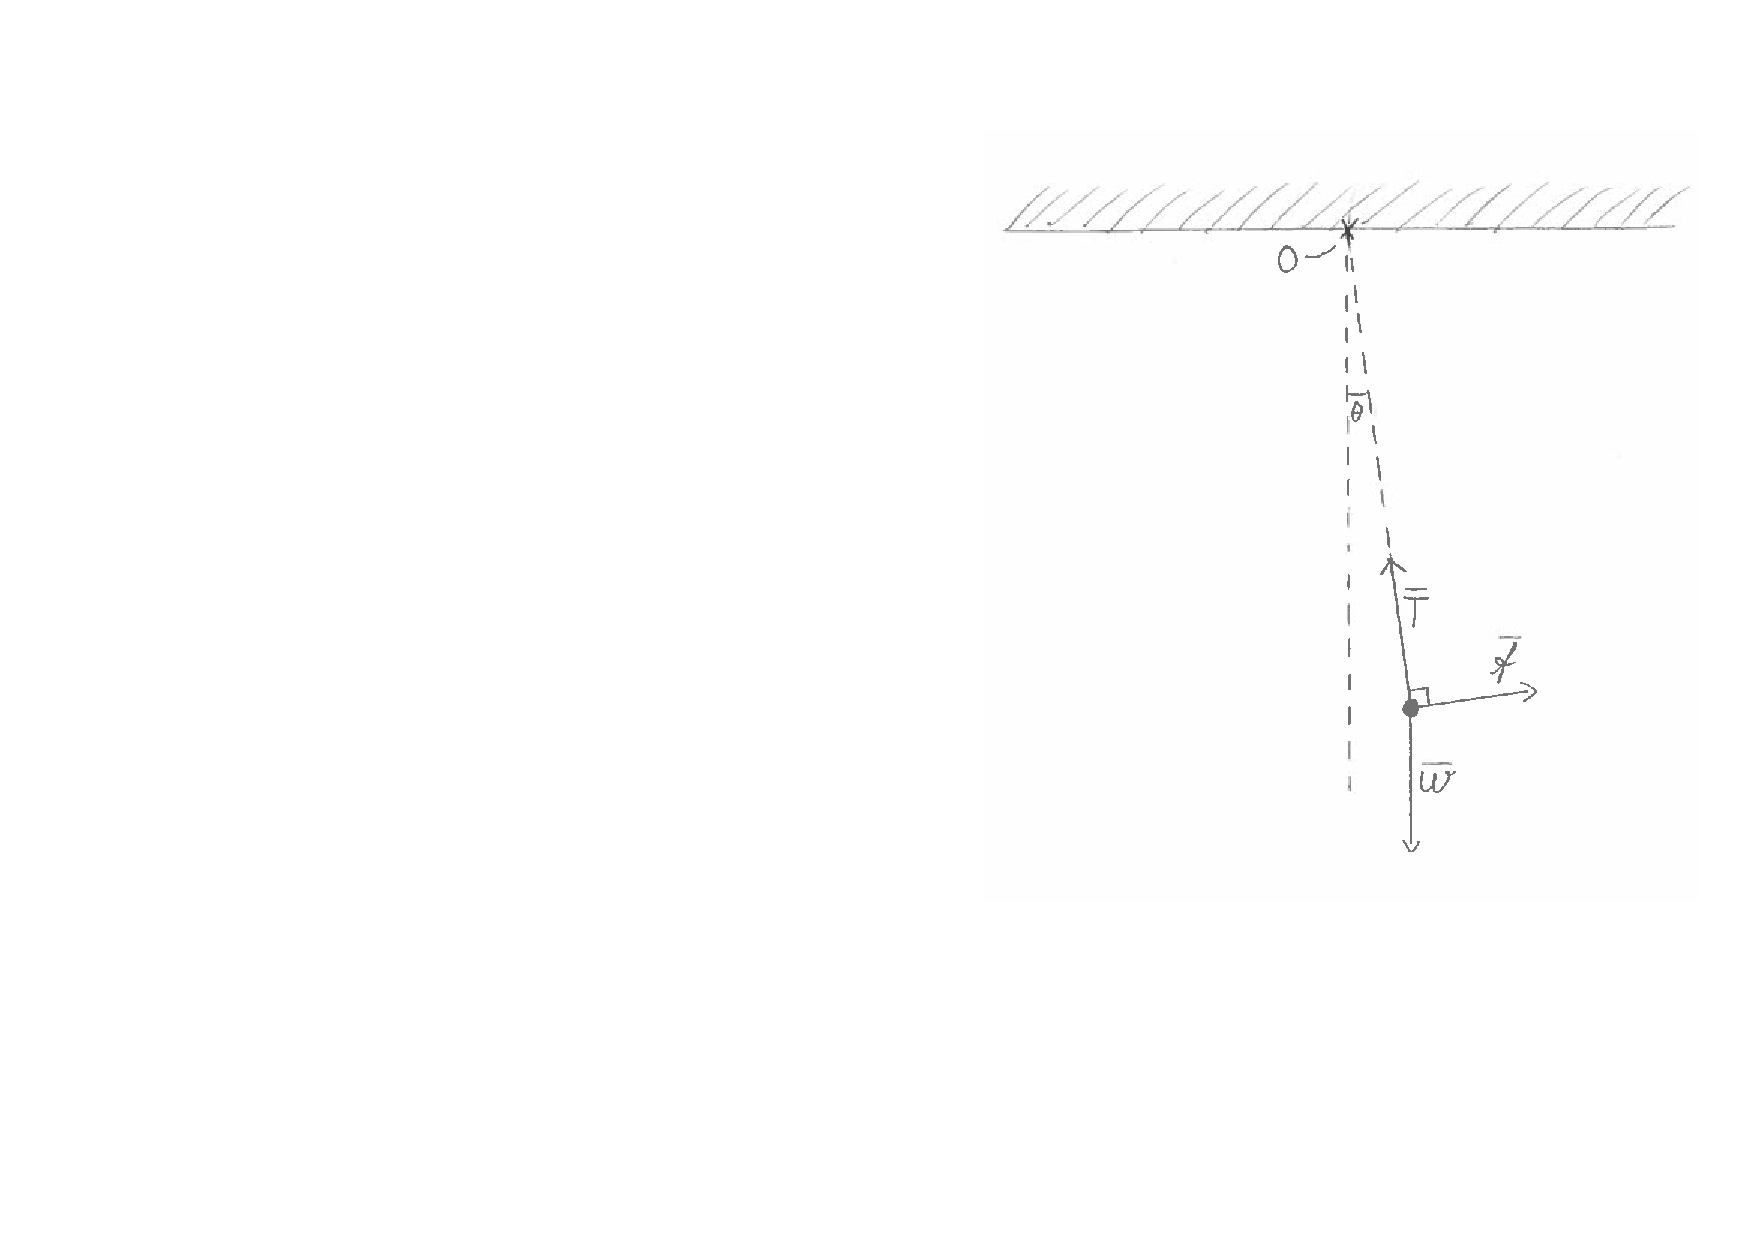
\includegraphics[width=\linewidth]{RotationelMekanik/Kraftanalyse}
  \caption{Kraftanalyse af de på pendulloddet virkende kræfter, der alle antages at have angrebspunkt i massemidtpunktet.}
  \label{fig:Kraftanalyse}
\end{subfigure}
\caption{Tegning af pendulet, der bl.a. viser det valgte koordinatsystem og de virkende kræfter.}
\end{figure}

I første omgang identificeres de på pendullodet virkende kræfter og pendulets ophængningspunkt defineres som origo, se figurene \ref{fig:Pendul} og \ref{fig:Kraftanalyse}. Pendullodets position beskrives ved en retningsvektor $\v{r}$, der går fra ophængningspunktet til lodet. Der er en tyngdekraft, $\v{w}$, en snorkraft, $\v{T}$, og en friktionskraft, $\v{f}$. Tyngdekraften virker til alle tider, $t$, i negativ $y$-retning og skrives derfor som
\begin{align*}
\v{w} = -mg\yhat
\end{align*}
hvor $g$ er tyngdeaccelerationen, og $\yhat$ er en enhedsvektor i $y$-retningen. Defineres $\boldsymbol{\hat{\textbf{r}}}$ som en enhedsvektor parallelt med pendulets retningsvektor, kan snorkraften beskrives som
\begin{align*}
\v{T} = -T\boldsymbol{\hat{\textbf{r}}}
\end{align*}
hvor $T$ er størrelsen på snorkraften. Friktionskraften virker antiparallelt med pendulets hastighed, $\v{v}$, hvorfor den kan beskrives med en skalering $b$ som
\begin{align*}
\v{f} = -b\v{v}
\end{align*}
Idet snoren antages masseløs kan pendulet beskrives som et lod med masse, $m$, der roterer omkring ophængningspunktet, og har ved denne rotation inertimomentet $I$. Snorens længde kaldes $L$ og alle kræfter antages at virke på loddets massemidtpunkt, hvorfor alle kræfters arm kan beskrives som
\begin{align*}
\v{r} = L\boldsymbol{\hat{\textbf{r}}}
\end{align*}
hvilket også et pendulloddets stedvektor. Nu kan kraftmomentet for alle de virkende kræfter bestemmes idet $\v{r}\perp\v{v}\enspace\forall t$
\begin{align*}
\gv{\tau}_w &= \v{r} \times \v{w} = -mgL \cdot \boldsymbol{\hat{\textbf{r}}} \times \yhat = -mgL\sin(\theta)\zhat \\
\gv{\tau}_f &= \v{r} \times \v{f} = -bL \cdot \boldsymbol{\hat{\textbf{r}}} \times \v{v} = -bLv\zhat = -bL^2\d{\theta}{t}\zhat \\
\gv{\tau}_T &= \v{r} \times \v{T} = -TL \cdot \boldsymbol{\hat{\textbf{r}}} \times \v{r} = \v{0}
\end{align*}
hvor subscriptet indikerer hvilken kraft, der behandles. Det samlede kraftmoment bliver derved
\begin{align*}
\sum\gv{\tau} = -\zhat\left(bL^2\d{\theta}{t} + mgL\sin\theta\right)
\end{align*}
Antages pendulets usvingsvinkel at være lille bliver det samlede kraftmomentets størrelse
\begin{align*}
\sum\tau \approx -\left(bL^2\d{\theta}{t} + mgL\theta\right)
\end{align*}
hvor Newtons anden lov for rotationel bevægelse giver differentialligningen
\begin{align*}
\dd{\theta}{t} = -\frac{1}{I}\left(bL^2\d{\theta}{t} + mgL\theta\right)
\end{align*}
som har løsningen
\begin{align*}
\theta(t) = A\exp\left(-\frac{bL^2}{2I}t\right)\cos\left(\omega t + \phi\right), \qquad \omega = \sqrt{\frac{mgL}{I} - \frac{b^2L^4}{4I^2}}
\end{align*}
hvilket medfører at pendulets periode bliver
\begin{align*}
T = \frac{2\pi}{\omega} = 2\pi\left(\frac{mgL}{I} - \frac{b^2L^4}{4I^2}\right)^{-1/2}
\end{align*}
Slutteligt kan pendulets $x$-koordinat beskrives som
\begin{align*}
x(t) = L\sin\theta(t) \approx L\theta(t)
\end{align*}

\subsection*{Simplificerende antagelser}
\subsubsection*{Matematisk pendul med friktion}
Antages lodet at være en punktmasse bliver dets inertimoment
\begin{align*}
I = mL^2
\end{align*}
hvorved  bevægelsesligningen bliver
\begin{align*}
\theta(t) = A\exp\left(-\frac{b}{2m}t\right)\cos\left(\omega t + \phi\right), \qquad \omega = \sqrt{\frac{g}{L} - \frac{b^2}{4m^2}}
\end{align*}
og perioden bliver nu
\begin{align*}
T = \frac{2\pi}{\omega} = 2\pi\left(\frac{g}{L} - \frac{b^2}{4m^2}\right)^{-1/2}
\end{align*}

\subsubsection*{Fysisk pendul uden friktion}
Negligeres friktionen bliver differentialligningen noget simplere, idet pendulet nu vil være i simpel harmonisk bevægelse
\begin{align*}
\dd{\theta}{t} = -\frac{mgL}{I}\theta
\end{align*}
som giver bevægelsesligningen
\begin{align*}
\theta(t) = A\cos\left(\omega t + \phi\right), \qquad \omega = \sqrt{\frac{mgL}{I}}
\end{align*}
og således bliver pendulets periode
\begin{align*}
T = \frac{2\pi}{\omega} = 2\pi\sqrt{\frac{I}{mgL}}
\end{align*}

\subsubsection*{Matematisk pendul uden friktion}
Negligeres friktion og antages pendulets masse at befinde sig i ét punkt kan intertimomentet sættes til $I=mL^2$ i ligningerne fra det fysiske pendul uden friktion
\begin{align*}
\theta(t) = A\cos\left(\omega t + \phi\right), \qquad \omega = \sqrt{\frac{g}{L}}
\end{align*}
hvilket giver en periode på
\begin{align*}
T = \frac{2\pi}{\omega} = 2\pi\sqrt{\frac{L}{g}}
\end{align*}
%Når du starter på en opgave skriver du \begin{opgave}{navnet på opgaven}{sværhedsgrad}, hvor sværhedsgraden skrives som 1,2 eller 3, hvor 3 er den sværeste. 
%Når opgaven er slut skrives \end{opgave}. 
%Såfremt der er delopgaver skrives delopgaver som \opg 

%Eksempel på opgave 
%\begin{opgave}{Polære koordinater}{1}
  %Den kinetiske energi af et legeme, der bevæger sig i 2D-planet er
  %i kartesiske koordinater ($x$ og $y$) givet ved ligning
  %(1.11).
  %
  %\opg Beregn $\dt{x}$ og $\dt{y}$ i polære koordinater og vis
  %derefter, at den kinetiske energi udtrykt i polære koordinater er
  %givet ved ligning (1.12).
%\end{opgave}

\chapter{Kerne-- og Partikelfysik Opgaver}

\section*{Kernefysik}
\begin{opgave}{Alfa-henfald}{1}
Alfa-henfald, hvor der udsendes en heliumkerne er en almindelig type henfald. F.eks. følgende henfald af Uran-238
\begin{equation*}
^{238}_{92} \text{U} \rightarrow ^{232}_{90}\text{Th} + ^{4}_{2}\text{He} .
\end{equation*}
\opg Hvorfor tror du netop udsendelsen af en alfa-partikel er en favoriseret type henfald? 
\opg Hvad er reaktionens $Q$-værdi? Ville denne reaktion forekomme naturligt?
Du kan anvende følgende atomare masser:
\begin{align*}
M(^{238}\text{U}) &=238,05079~\SI{}{u} \\
M(^{234}\text{Th}) &= 234,04360~\SI{}{u} \\
M(^4\text{He}) &= 4,002602~\SI{}{u} \\
\end{align*}
.
\end{opgave}

\begin{opgave}{Berylliums isotoper}{2}
Det lette grundstof beryllium har i alt otte isotoper, hvoraf kun Be-9 er stabil. \\
\opg Sammenlign den atomare masse af Be-8 med massen af to He-4. Hvad kan man konkludere herfra? 
\opg Sammenlign også den atomare masse af Be-9 med massen af $^7\text{Li}$ og $^2\text{H}$. Hvad fortæller dette dig?

Du kan anvende følgende masser:
\begin{align*}
M(^2\text{H}) &= 2,014102~\SI{}{u}\\
M(^4\text{He}) &= 4,002602~\SI{}{u} \\
M(^7\text{Li}) &= 7,016003~\SI{}{u} \\
M(^8\text{Be}) &= 8,005305~\SI{}{u} \\
M(^9\text{Be}) &= 9,012174~\SI{}{u}
\end{align*} 
\end{opgave}

\begin{opgave}{Kerners tæthed}{3}
\label{opg:density}
En atomkerne kan antages at være en kugle, sådan at volumen er givet som $V=\frac{4}{3} \pi R^3$. Vis, at tætheden af en kerne ikke afhænger af grundstoffet, altså at tætheden er ens for alle kerner. \emph{Hint: anvend at massen af en kerne i atomare masseenheder ca. er lig massetallet for kernen, altså at $m\approx A$}.
\end{opgave}

\begin{opgave}{Den stærkest bundne kerne}{1}
\label{opg:nickel}
$^{62}\text{Ni}$ har den højeste bindingsenergi per nukleon af alle kerner. 
\opg Hvor meget energi skal der til for at splitte kernen ad?
Anvend at den atomare masse af $^{62}\text{Ni}$ er $61,928349~\SI{}{u}$.
\end{opgave}

\begin{opgave}{Splittelsen af en kerne}{1}
Antag følgende reaktion:
\begin{equation*}
^{28}_{14} \text{Si} + \gamma \rightarrow ^{24}_{12}\text{Mg} + X,
\end{equation*}

hvor $X$ er en kerne.
\opg hvad er $A$ og $Z$ for $X$?
\opg hvis vi antager at energien af fotonen ikke går til kinetisk energi for $^{24}_{12}\text{Mg}$ og $X$, hvad er så dens energi? Anvend at massen af et Si-28-atom er $27,976927~\si{u}$ og at massen af et Mg-24-atom er $23,985042~\si{u}$
\end{opgave}

\begin{opgave}{Fusion i Solen}{2}
Stjerner som Solen skinner på grund af den fusion som foregår i deres kerner. Temperaturen i stjernernes kerner er så høje, at elektronerne er frie, altså ikke bundet til atomer. I Solen omdannes 4 protoner gennem en række skridt (kaldet pp-kæden) til én $^{4}\text{He}$-kerne. Helt overordnet kan reaktionen skrives som:
\begin{equation*}
4p \rightarrow \alpha + 2e^+ + 2\nu_e + E,
\end{equation*}
Dvs. der bliver desuden dannet to positroner og 2 elektronneutrinoer samt en mængde energi.
\opg Hvor meget energi dannes i ovenstående reaktion? Antag at elektronneutrinoens masse er 0. Du kan anvende \emph{ den atomare masse} af helium: $M(^4\text{He})= 4,002602~\SI{}{u}$.
\opg pp-kæden starter ved at to protoner mødes. Men i kraft af deres ladning vil de frastøde hinanden, og de skal derfor have tilstrækkelig bevægelsesenergi for at det kan lade sig gøre. Det elektriske potential (barrieren) mellem to ladede partikler er givet ved:
\begin{equation}
U = \frac{1}{4\pi \epsilon_0} \frac{q_1q_2}{r}.
\end{equation}
Potentialet $U$ er i joule, hvis ladningerne af partiklerne angives i coulomb.
Antag at den stærke kernekraft overvinder den elektriske frastødning når de to protoner kommer i afstanden af $1,4 \cdot 10^{-15}$m fra hinanden. Hvad er den samlede minimale energi af protonerne?
\opg Det er kun muligt for atomer og partikler at have så høje energier ved virkelig høje temperaturer. Den gennemsnitlige energi af partikler og temperaturen af det medie, de befinder sig i, er relateret til hinanden via:
\begin{equation}
E = \frac{3}{2} k T,
\end{equation}
hvor $k$ er Boltzmanns konstant og $T$ er temperaturen i grader Kelvin. Hvad er temperaturen svarende til energien du fandt i foregående opgave? Solens kernetemperatur er ca. $1,5 \cdot 10^7$K. Hvordan sammenlignes det med dit resultat?
\opg NB: sjov opgave!
Vi kan prøve at antage, at al energien der bliver produceret i ovenstående reaktion bliver båret væk af neutrinoer. Lad os også antage at al Solens udstråling bliver skabt ved ovenstående reaktion. Ved Jordens overflade modtages Solens udstråling (kaldet solkonstanten $S_0$) ved værdien: $S_0 = 1,362 \cdot 10^3 J m^{-2}s^{-1}$. Hvor mange neutrinoer fra Solen rammer en kvadratcentimeter af Jordens overflade hvert sekund? Hvor mange solneutrinoer rammer spidsen af din finger hvert sekund?
\end{opgave}

\begin{opgave}{Dannelse af tunge grundstoffer i en supernova: r- og s-proces}{2}
Stjerner kan kun fusionere grundstoffer op til jern. Figur \ref{fig:fusion} viser tværsnittet af en tung stjerne som befinder sig i slutningen af dens levetid.
\begin{figure}[h]
  \centering
  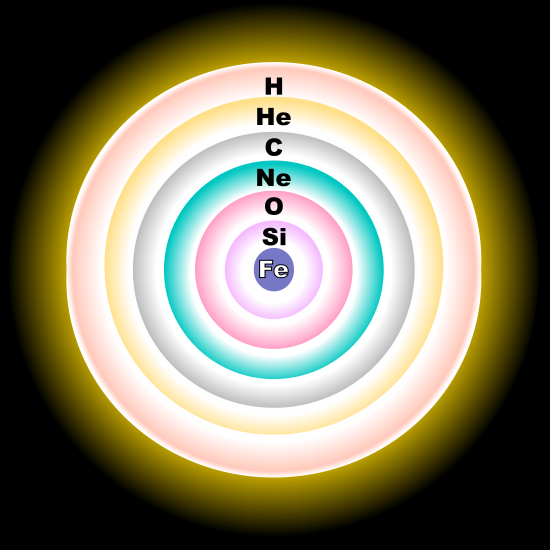
\includegraphics[scale=0.3]{KernePartikel/fusion.png}
  \caption{Skalstruktur i stjerner}
  \label{fig:fusion}
\end{figure}
\opg Forklar løgstruktur-udseendet af stjernen. Hvad er grunden til at stjerner ikke kan danne elementer tungere end jern ved fusion?

Elementer tungere end jern må da være dannet andetsteds end i stjernernes indre. Et miljø, hvor der dannes tunge grundstoffer er de energirige supernova-eksplosioner. Her bliver grundstofferne ikke dannet ved fusion, men ved neutron-indfangning og senere $\beta^-$-henfald af kernen. Det kunne f.eks. foregå på følgende måde:
\begin{equation*}
^{A}_{Z} \text{X}_{N} + n \rightarrow  ^{A+1}_{Z}\text{X}_{N+1} \rightarrow ^{A+1}_{Z+1}\text{Y}_{N} + e^- + \bar{\nu}_e
\end{equation*}

I en supernova-eksplosion skabes en kæmpe mængde neutroner, som gør neutron-indfangning muligt. Men kerner med ekstra neutroner er ustabile og vil henfalde ved hjælp af $\beta^-$-henfald. Derfor kan man sige, at neutron-indfangningen og henfaldene konkurrerer med hinanden. Hvis neutron-indfangningen kan ske hurtigere end kernen kan nå henfalde kaldes det for en r-proces ("r" for \emph{eng: rapid} - hurtig). Hvis kernen når at henfalde inden den kan indfange en ny neutron kaldes det for en s-proces ("s" for \emph{eng: slow} - langsom). \\

Figur \ref{fig:sn} viser et udsnit af kernekortet omkring $N \sim 100$ og $Z \sim 70$. 


De sorte firkanter repræsenterer kerner som er stabile, og derfor ikke kan undergå henfald. 
\opg Hvordan ændrer en kerne sig på kortet hvis den fanger én neutron? Hvordan ændrer en kerne sig på kortet hvis den undergår $\beta^-$-henfald?
\opg Start ved kernen 181-Ta. Antag at kernen undergår 5 neutron-indfangninger ved r-proces. Hvilken kerne bliver dannet (til sidst?)
\opg Antag nu at kernen undergår 5 neutron-indfangninger ved s-proces. Hvilken kerne bliver dannet?
\opg Kan kernen 180-Ta dannes ved neutronindfangning? Forklar dit svar.
\end{opgave}
\begin{figure}[h]
	\centering
	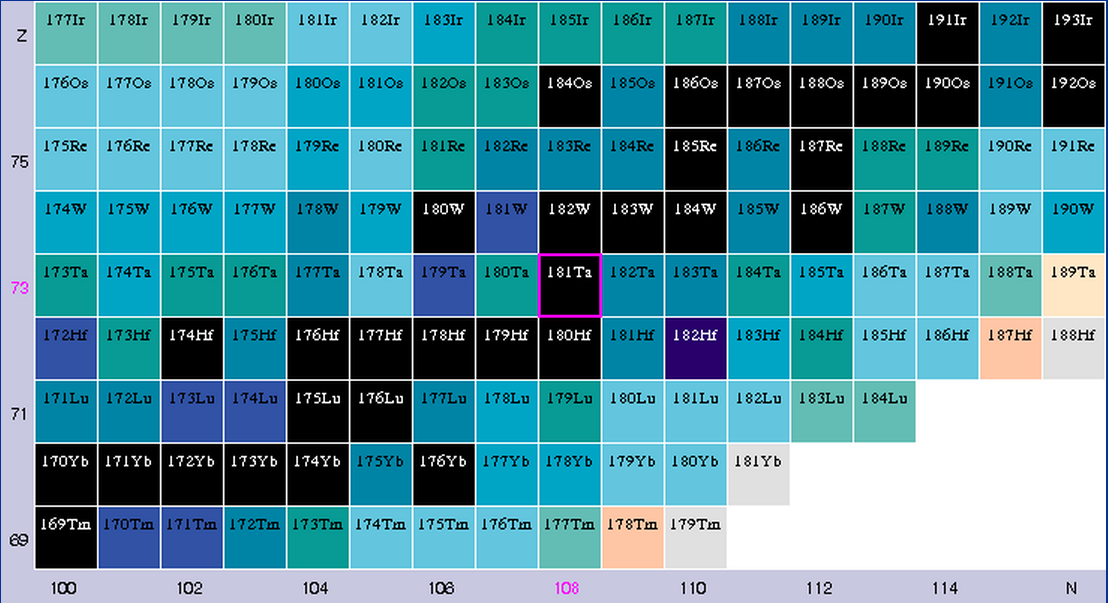
\includegraphics[width=\textwidth]{KernePartikel/supernova_chart.png}
	\caption{Et udsnit af kernekortet}
	\label{fig:sn}
\end{figure}
\newpage

\section*{Partikelfysik}

\begin{opgave}{Bevarelseslove}{1}
\opg Hvilke bevarelseslove gør sig gældende i partikelfysik?\\
\opg Kig på følgende reaktioner og bestem, om de kan lade sig gøre eller ej.
\begin{enumerate}
\item $e^- \longleftrightarrow e^- + e^+ + e^+$
\item $p + n \longleftrightarrow e^- + e^+ + e^+$
\item $p + n + e^+ \longleftrightarrow n + p + \bar{\nu}_e$
\item $p \longleftrightarrow \mu^- + n + \bar{\nu}_\mu $
\item $p \longleftrightarrow \mu^+ + n + \nu_\mu $
\item $\bar{n} \longleftrightarrow \bar{p} + e^+ + \nu_e$
\item $e^- + \mu^+ \longleftrightarrow n$
\end{enumerate}
\emph{Hint: tjek om bevarelseslovene er opfyldt.}
\end{opgave}

\begin{opgave}{Dannelse af to muoner}{1}
Tegn et feynman-diagram, hvor en foton danner muoner i en pardannelsesproces. Hvad er den minimalt krævede energi af fotonen? 
\end{opgave}

\begin{opgave}{Reaktioner med $W^\pm$-partiklen}{2}
\label{opg:W}
Betragt reaktionen i Figur \ref{fig:Wvertex}.
\begin{figure}[h]
  \centering
  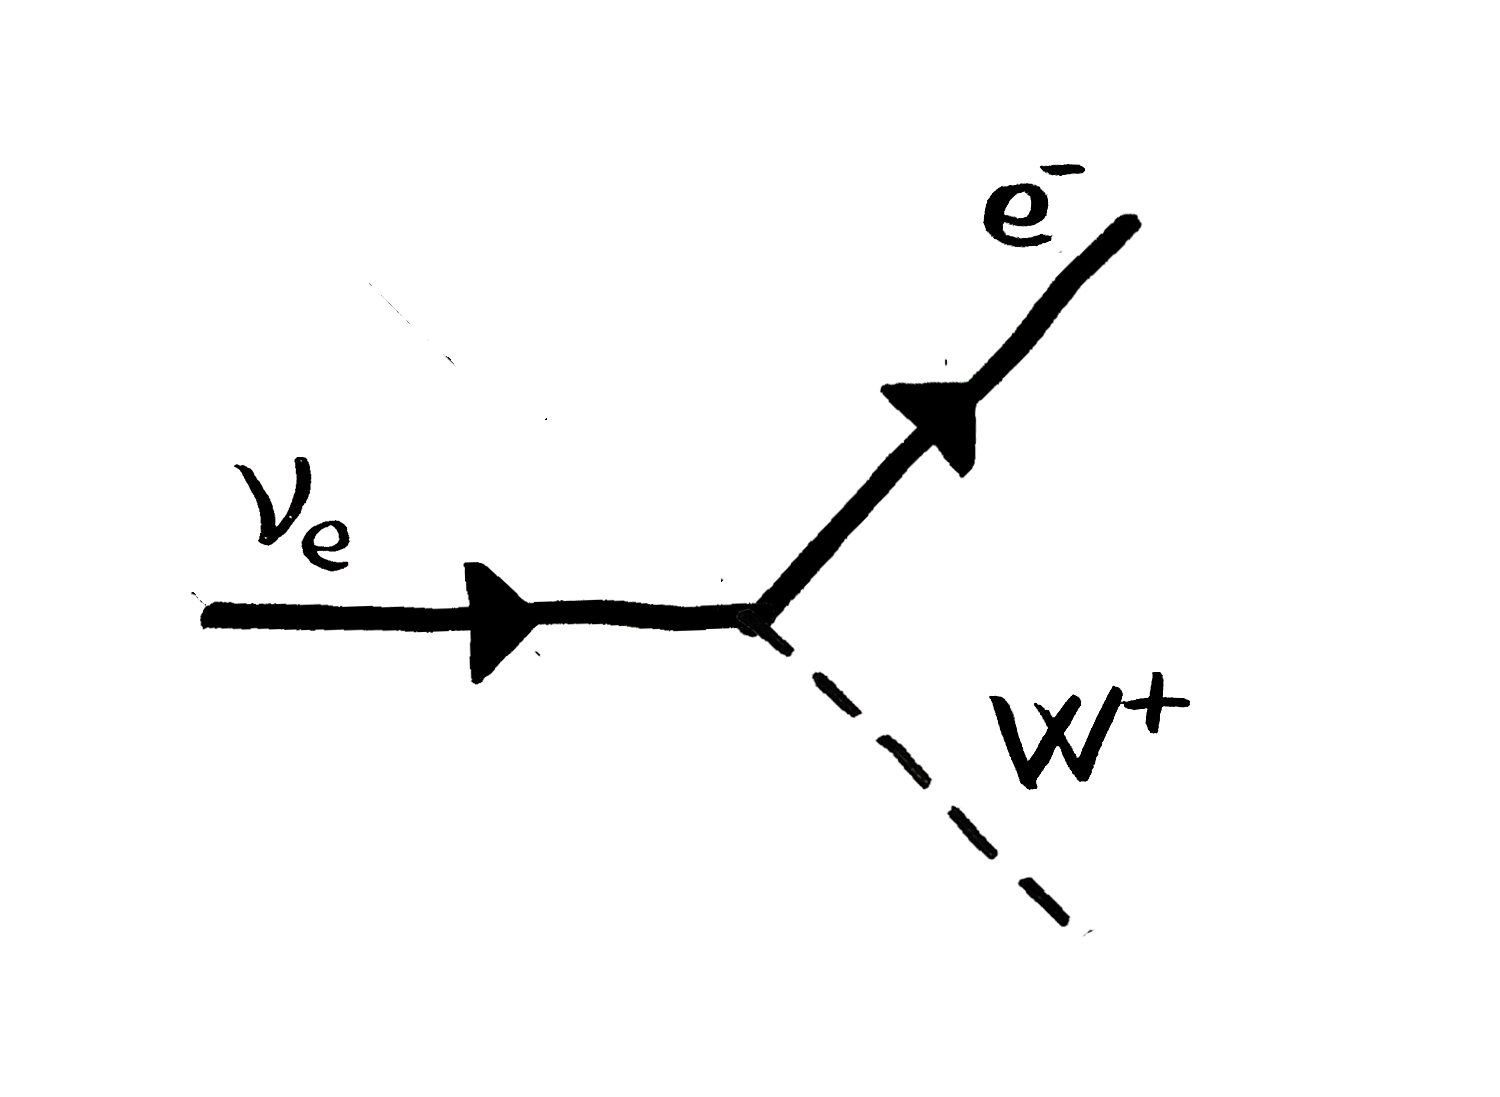
\includegraphics[width=0.3\textwidth]{KernePartikel/weak_vertex.png}
  \caption{Udsendelse af en $W^+$-boson.}
  \label{fig:Wvertex}
\end{figure}
\opg
Rotér feynmandiagrammet mod uret så det viser en indkommende positron i stedet. Hvad slags neutrino produceres der? Hvad er nu ladningen af $W$-bosonen?
\opg
Udskift positronen med en elektron. Hvad slags neutrino produceres der og hvad er ladningen af $W$-bosonen?

Feynman--diagrammet for et beta--minus--henfald er vist
i Figur \ref{fig:beta_minus}.
\begin{figure}[h]
  \centering
  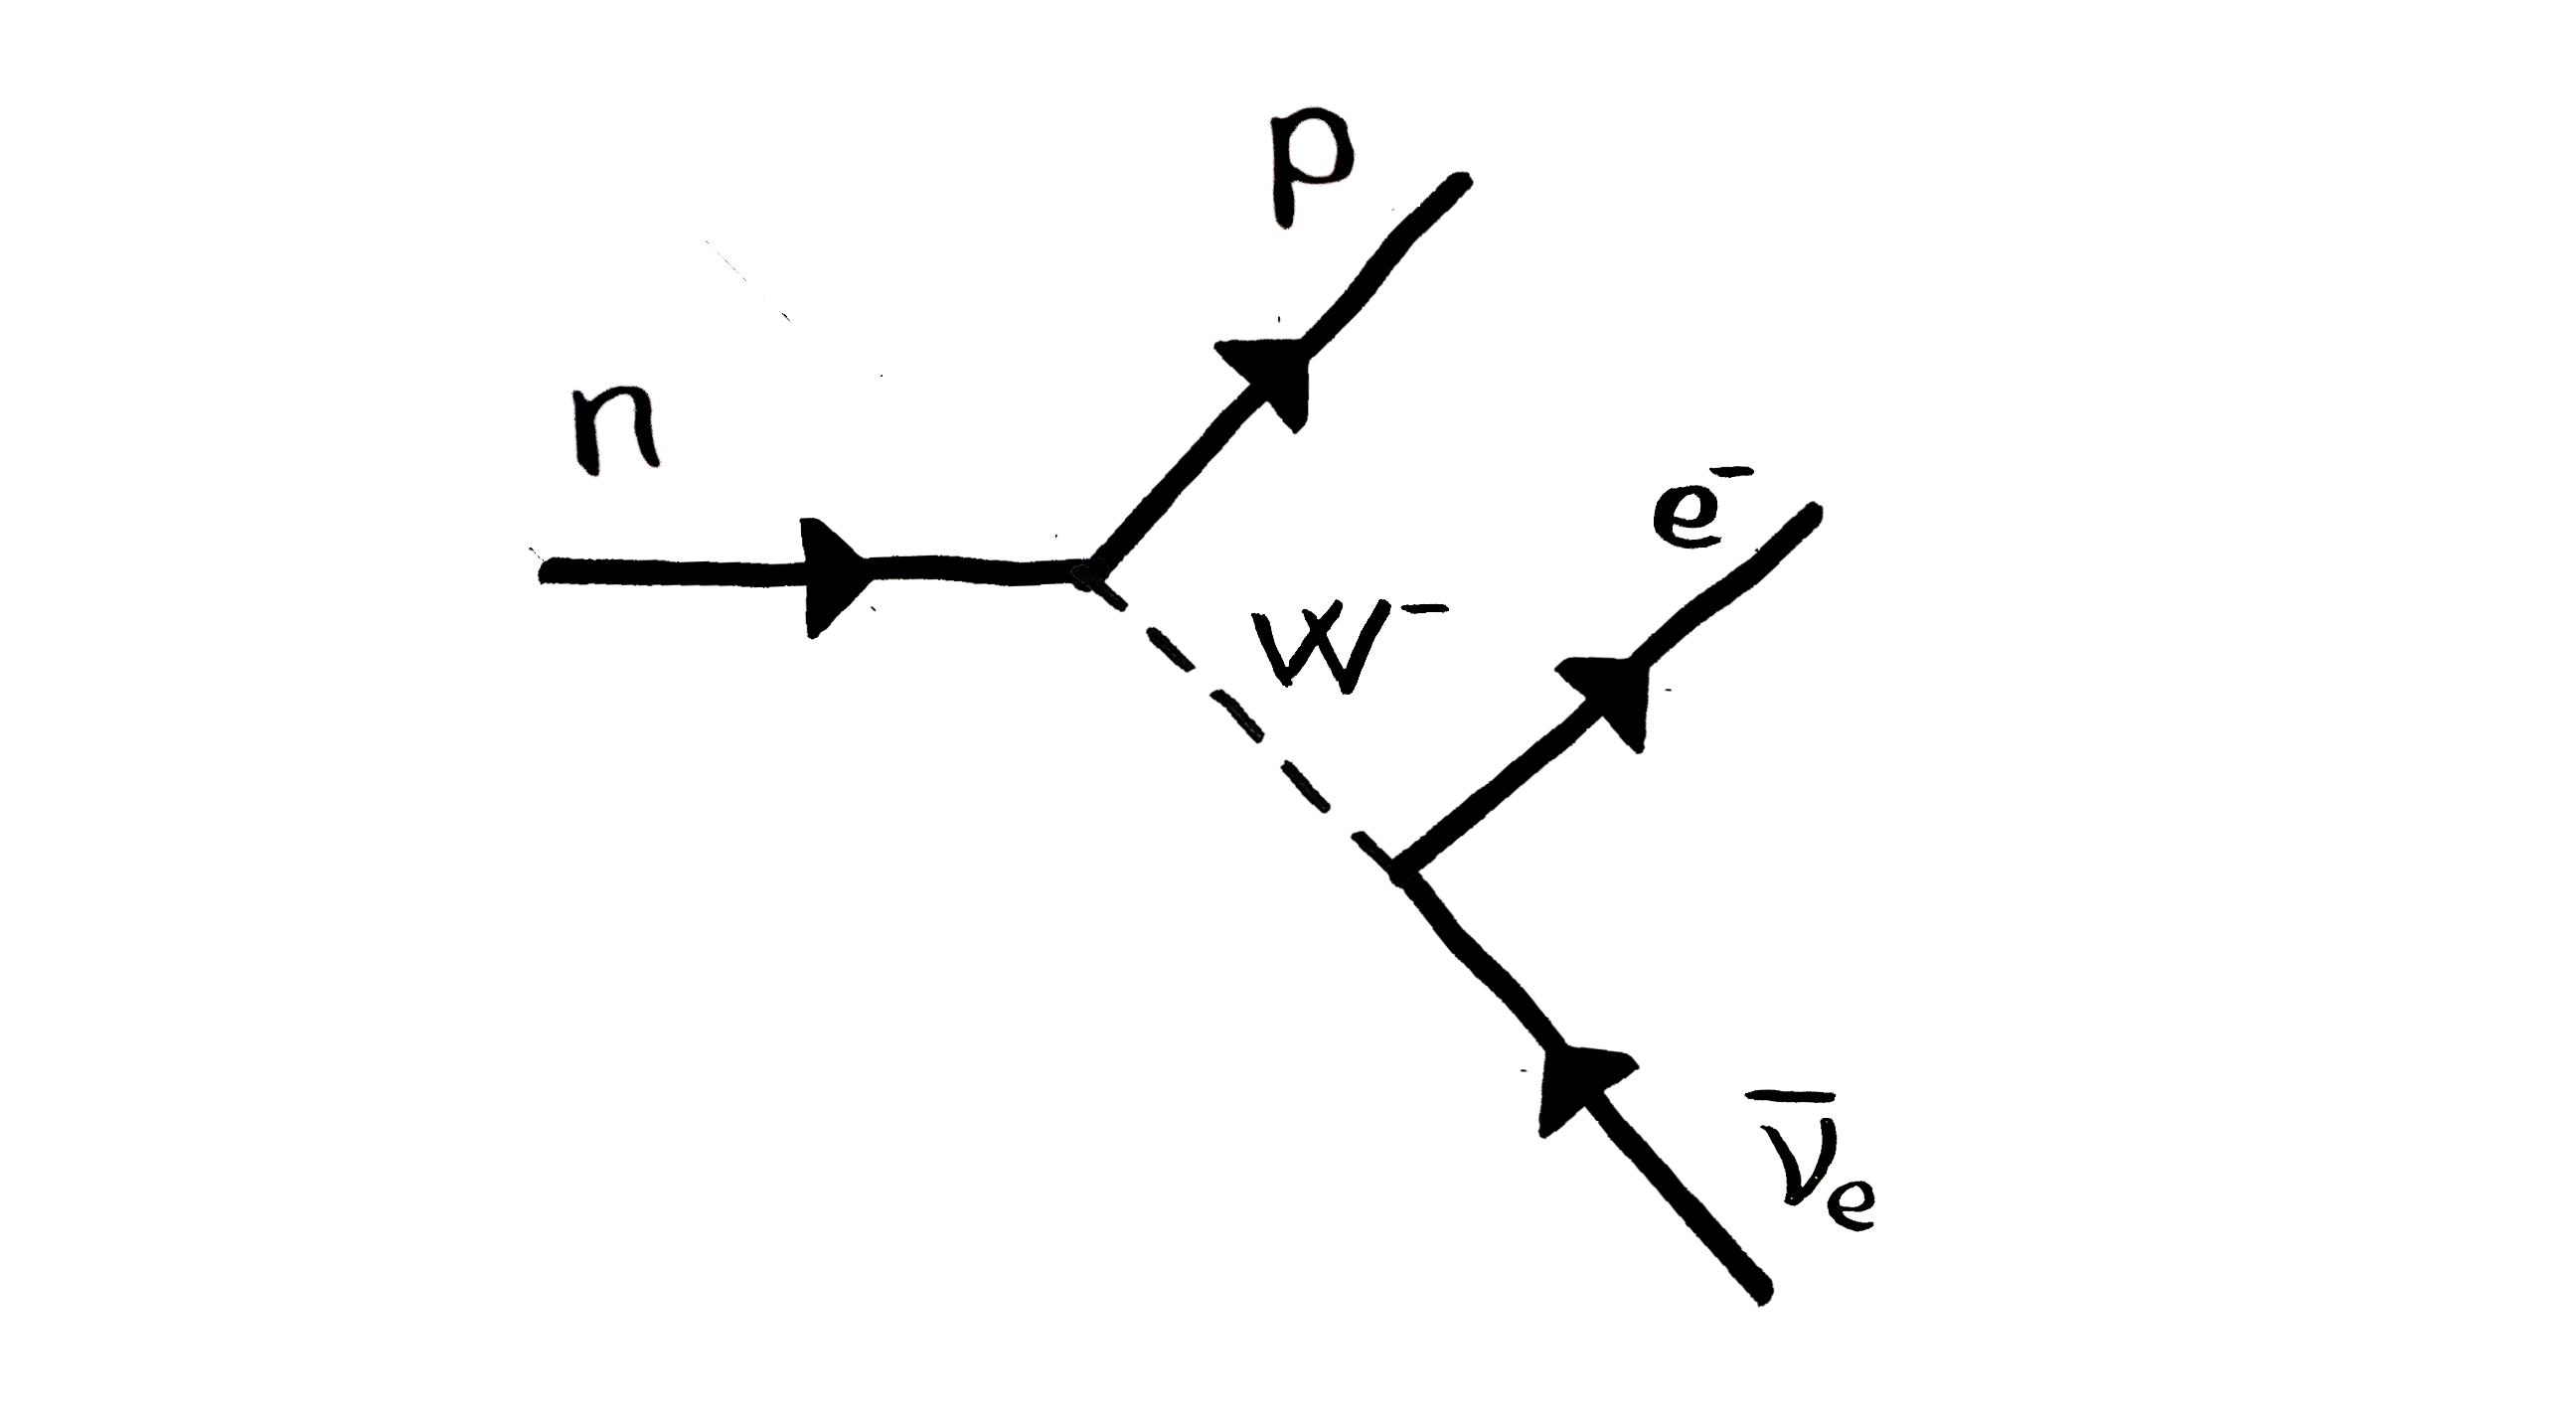
\includegraphics[width=0.6\textwidth]{KernePartikel/beta_minus.png}
  \caption{Beta-minus-henfald.}
  \label{fig:beta_minus}
\end{figure}
\opg Tegn feynman-diagrammet for et beta-plus-henfald: $p \rightarrow
n + e^+ + \nu_e$.
\opg Tegn feynman-diagrammet for en elektron-indfangning: $p + e^-
\rightarrow n + \nu_e$.

Som nævnt i kompendiet består neutronen og protonen af kvarker, som kan omdannes ved hjælp af $W$-bosonen, så deres ladningen ændres med enten $\pm$ 1, f.eks. u$\longleftrightarrow$ d. Figur \ref{fig:Wquarks} viser en oversigt over kvarkerne, hvor pilen mellem u-- og d-- kvarken betyder, at $W$-bosonen kan ændre disse kvarker til hinanden. 
\begin{figure}[h!]
  \centering
  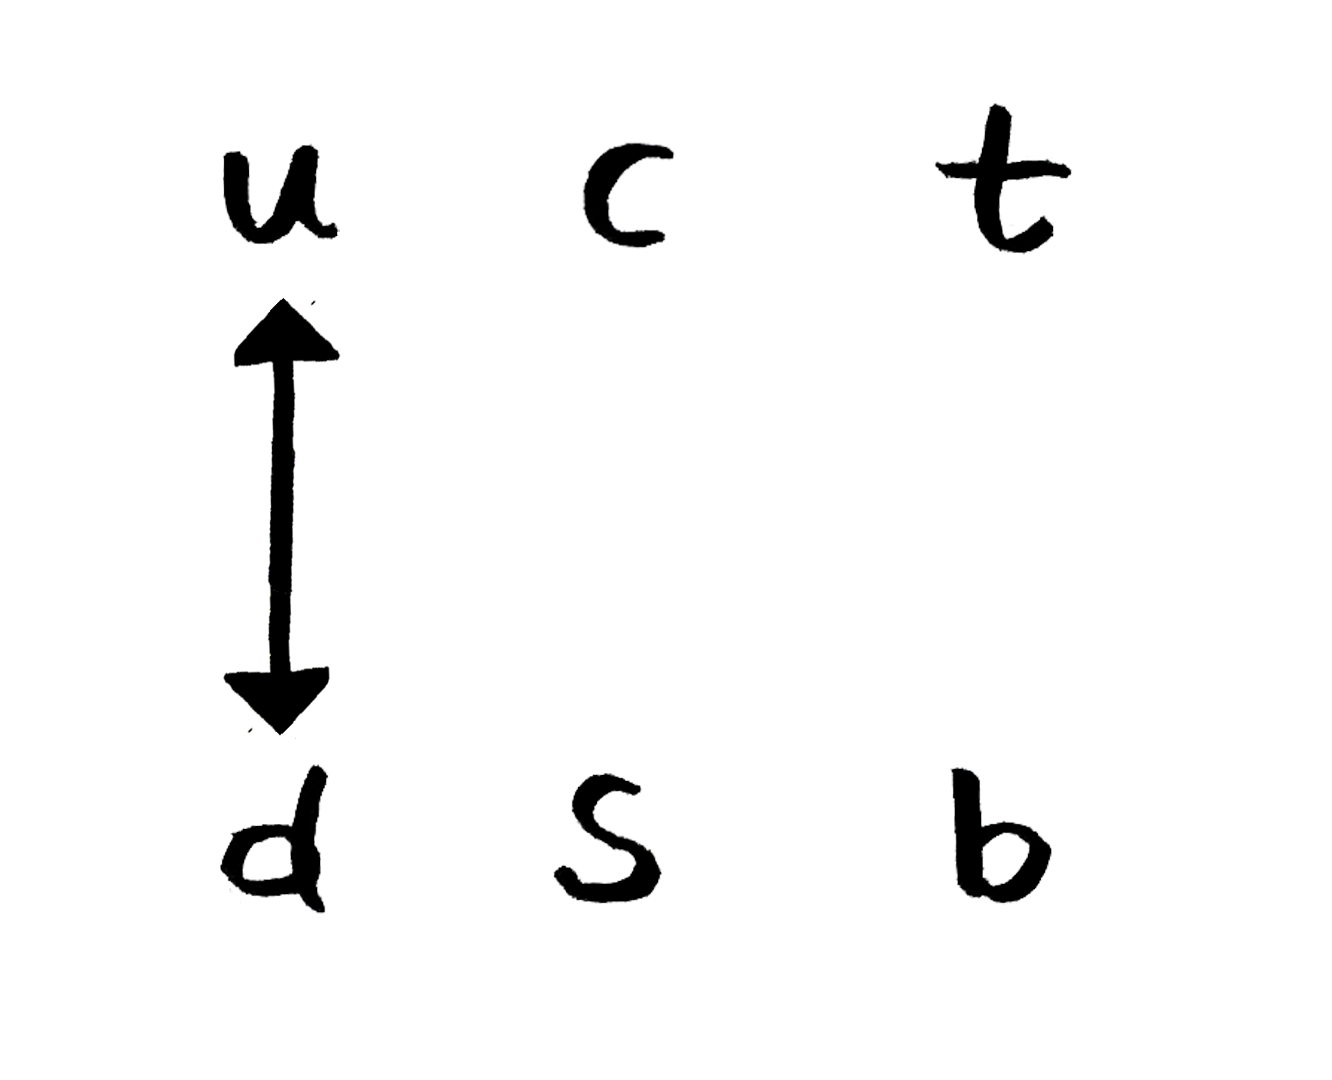
\includegraphics[width=0.3\textwidth]{KernePartikel/Wquarks.png}
  \caption{$W$-bosonen kan ændre kvarker til en anden type så længe ladningen ændres med $\pm 1$}
  \label{fig:Wquarks}
\end{figure}
\opg Indtegn på figur \ref{fig:Wquarks} pile mellem alle de kvarker, som $W$ kan omdanne. 
\opg En t-kvark omdannes til en b-kvark under udsendelse af en $W$-partikel. Tegn feynman-diagrammet. Hvad er ladningen af $W$?
\opg En s-kvark og en anti-c kvark annihilerer og skaber en $W$-partikel. Tegn feynman-diagrammet. Hvad er ladningen af $W$?
\opg Tegn feynmandiagrammet for et beta-minus-henfald, men denne gang tegn neutronens og protonens kvarker som en del af reaktionen. \emph{Hint: partikler kan sagtens optræde uændret i et feynman-diagram.}
\end{opgave}

\begin{opgave}{Feynman-diagrammer: en sand kunstart}{3}
\label{opg:feynman1}
\emph{NB: det er en god idé at lave opgave \ref{opg:W} inden denne opgave.}

Før vi er helt klar til at give os i kast med en masse
feynman-diagrammer, skal gluonen ($g$) introduceres. Gluonen, som
bærer den stærke vekselvirkning, virker ved at ændre en egenskab ved
kvarkerne kaldet \emph{farve}. Feltet som beskæftiger sig med dette
kaldes for kvantekromodynamik, og det er det, som beskriver hvorfor
kvarkerne kun kan eksistere i grupper af tre (hadronerne) og to
(mesonerne). Kvantekromodynamik er dog en anelse ud over niveauet for
denne camp, men det forhindrer os ikke i at gøre brug af gluonen i
vores feynman-diagrammer.
\begin{figure}[h!]
  \centering
  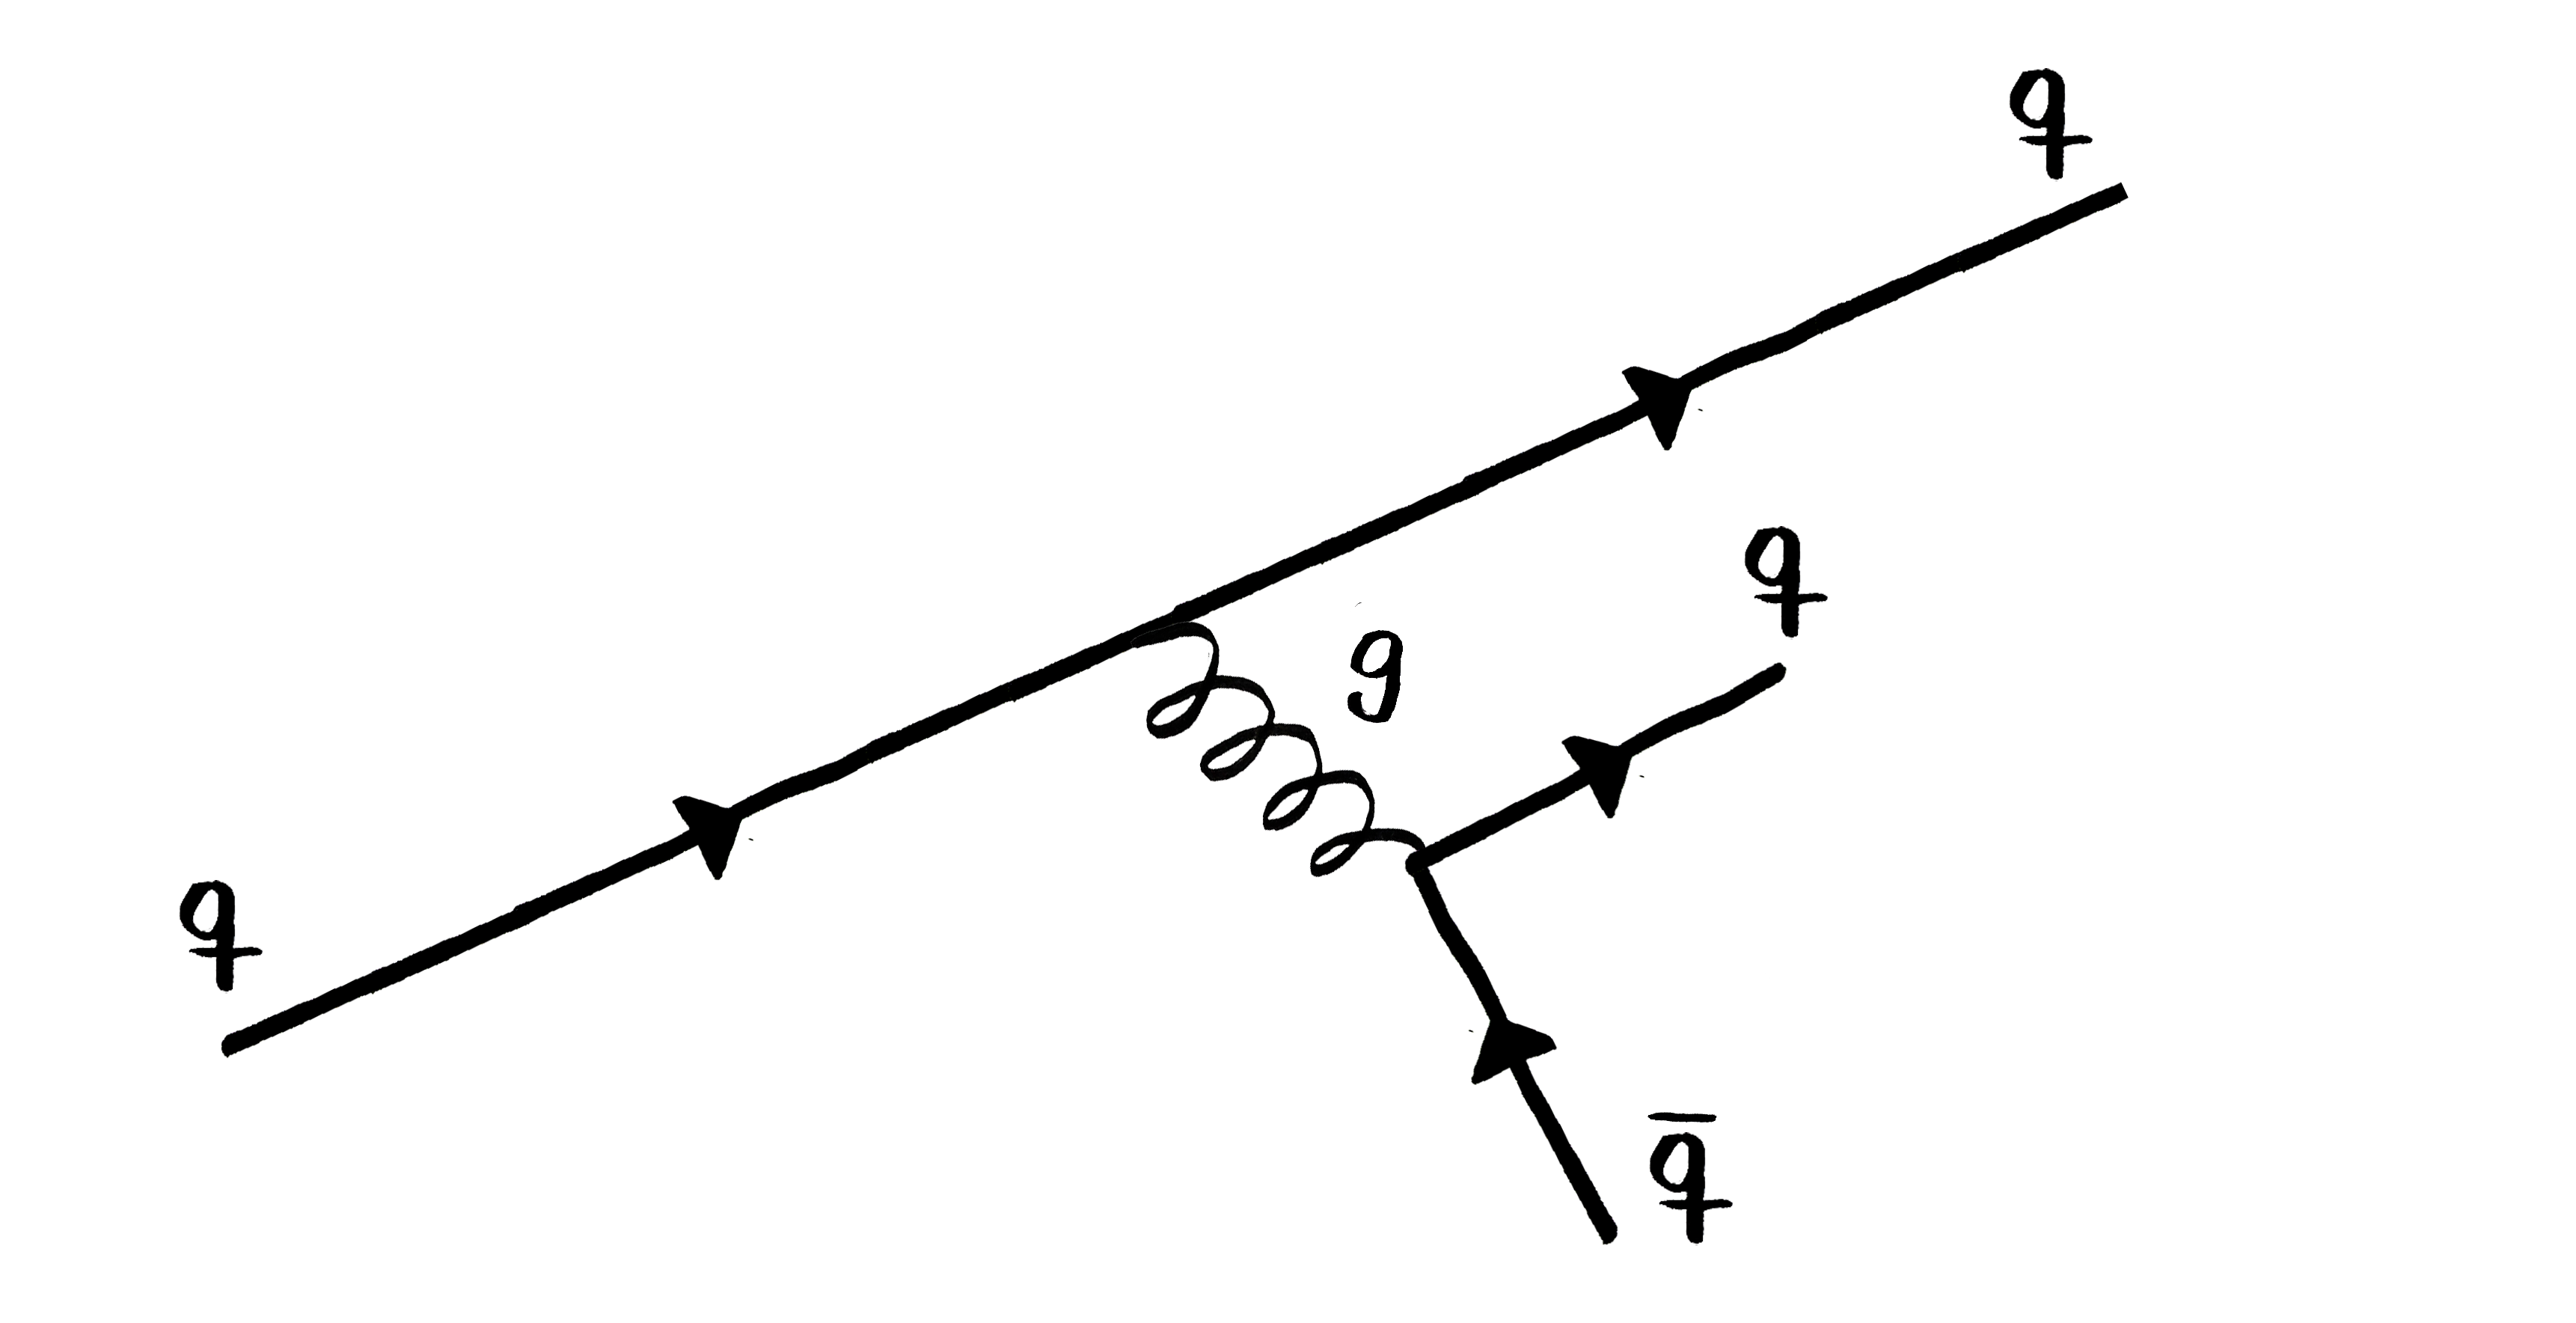
\includegraphics[width=0.6\textwidth]{KernePartikel/quark_interaction.png}
  \caption{Reaktion med gluonen $g$.}
  \label{fig:quark_inter}
\end{figure}
Figur \ref{fig:quark_inter} viser en typisk vekselvirkning med
gluonen, som normalt tegnes som en fjederform. Heri udsender en
vilkårlig kvark en gluon og fortsætter. Kvarktypen ændrer sig ikke
under udsendelse af en gluon (kun dens farve, men igen, det behøver vi
ikke tage højde for). Gluonen henfalder til et vilkårligt
kvark-antikvark-par. Gluonens energi afgør, hvilket
kvark-antikvark-par der kan dannes, men u- og d-kvarken er de mindst
energirige (mindst massive) og kan derfor altid dannes med høj
sandsynlighed. Det betyder, at det er ''gratis'' at introducere en gluon
i dit feynman-diagram, som enten henfalder til et u$\bar{\text{u}}$-
eller d$\bar{\text{d}}$-par.

Nu skal vi sætte vores nylærte
egenskaber til prøve med henfald af sammensatte partikler. Som
eksempel kigger vi på henfaldet:
\begin{equation*}
D^- \rightarrow K^+ + \pi^- + \pi^-.
\end{equation*}
Dette er henfaldet af $D^-$-mesonen (kvarksammensætning: d$\bar{\text{c}}$ ) til mesonerne $K^+$ (u$\bar{\text{s}}$), og to $\pi^-$ (d$\bar{\text{u}}$). Et sådant henfald er vist i figur \ref{fig:D_reaction}. Læg mærke til, at man kan sætte klammer om de kvarker, der hører sammen i en partikel.
\begin{figure}[h!]
  \centering
  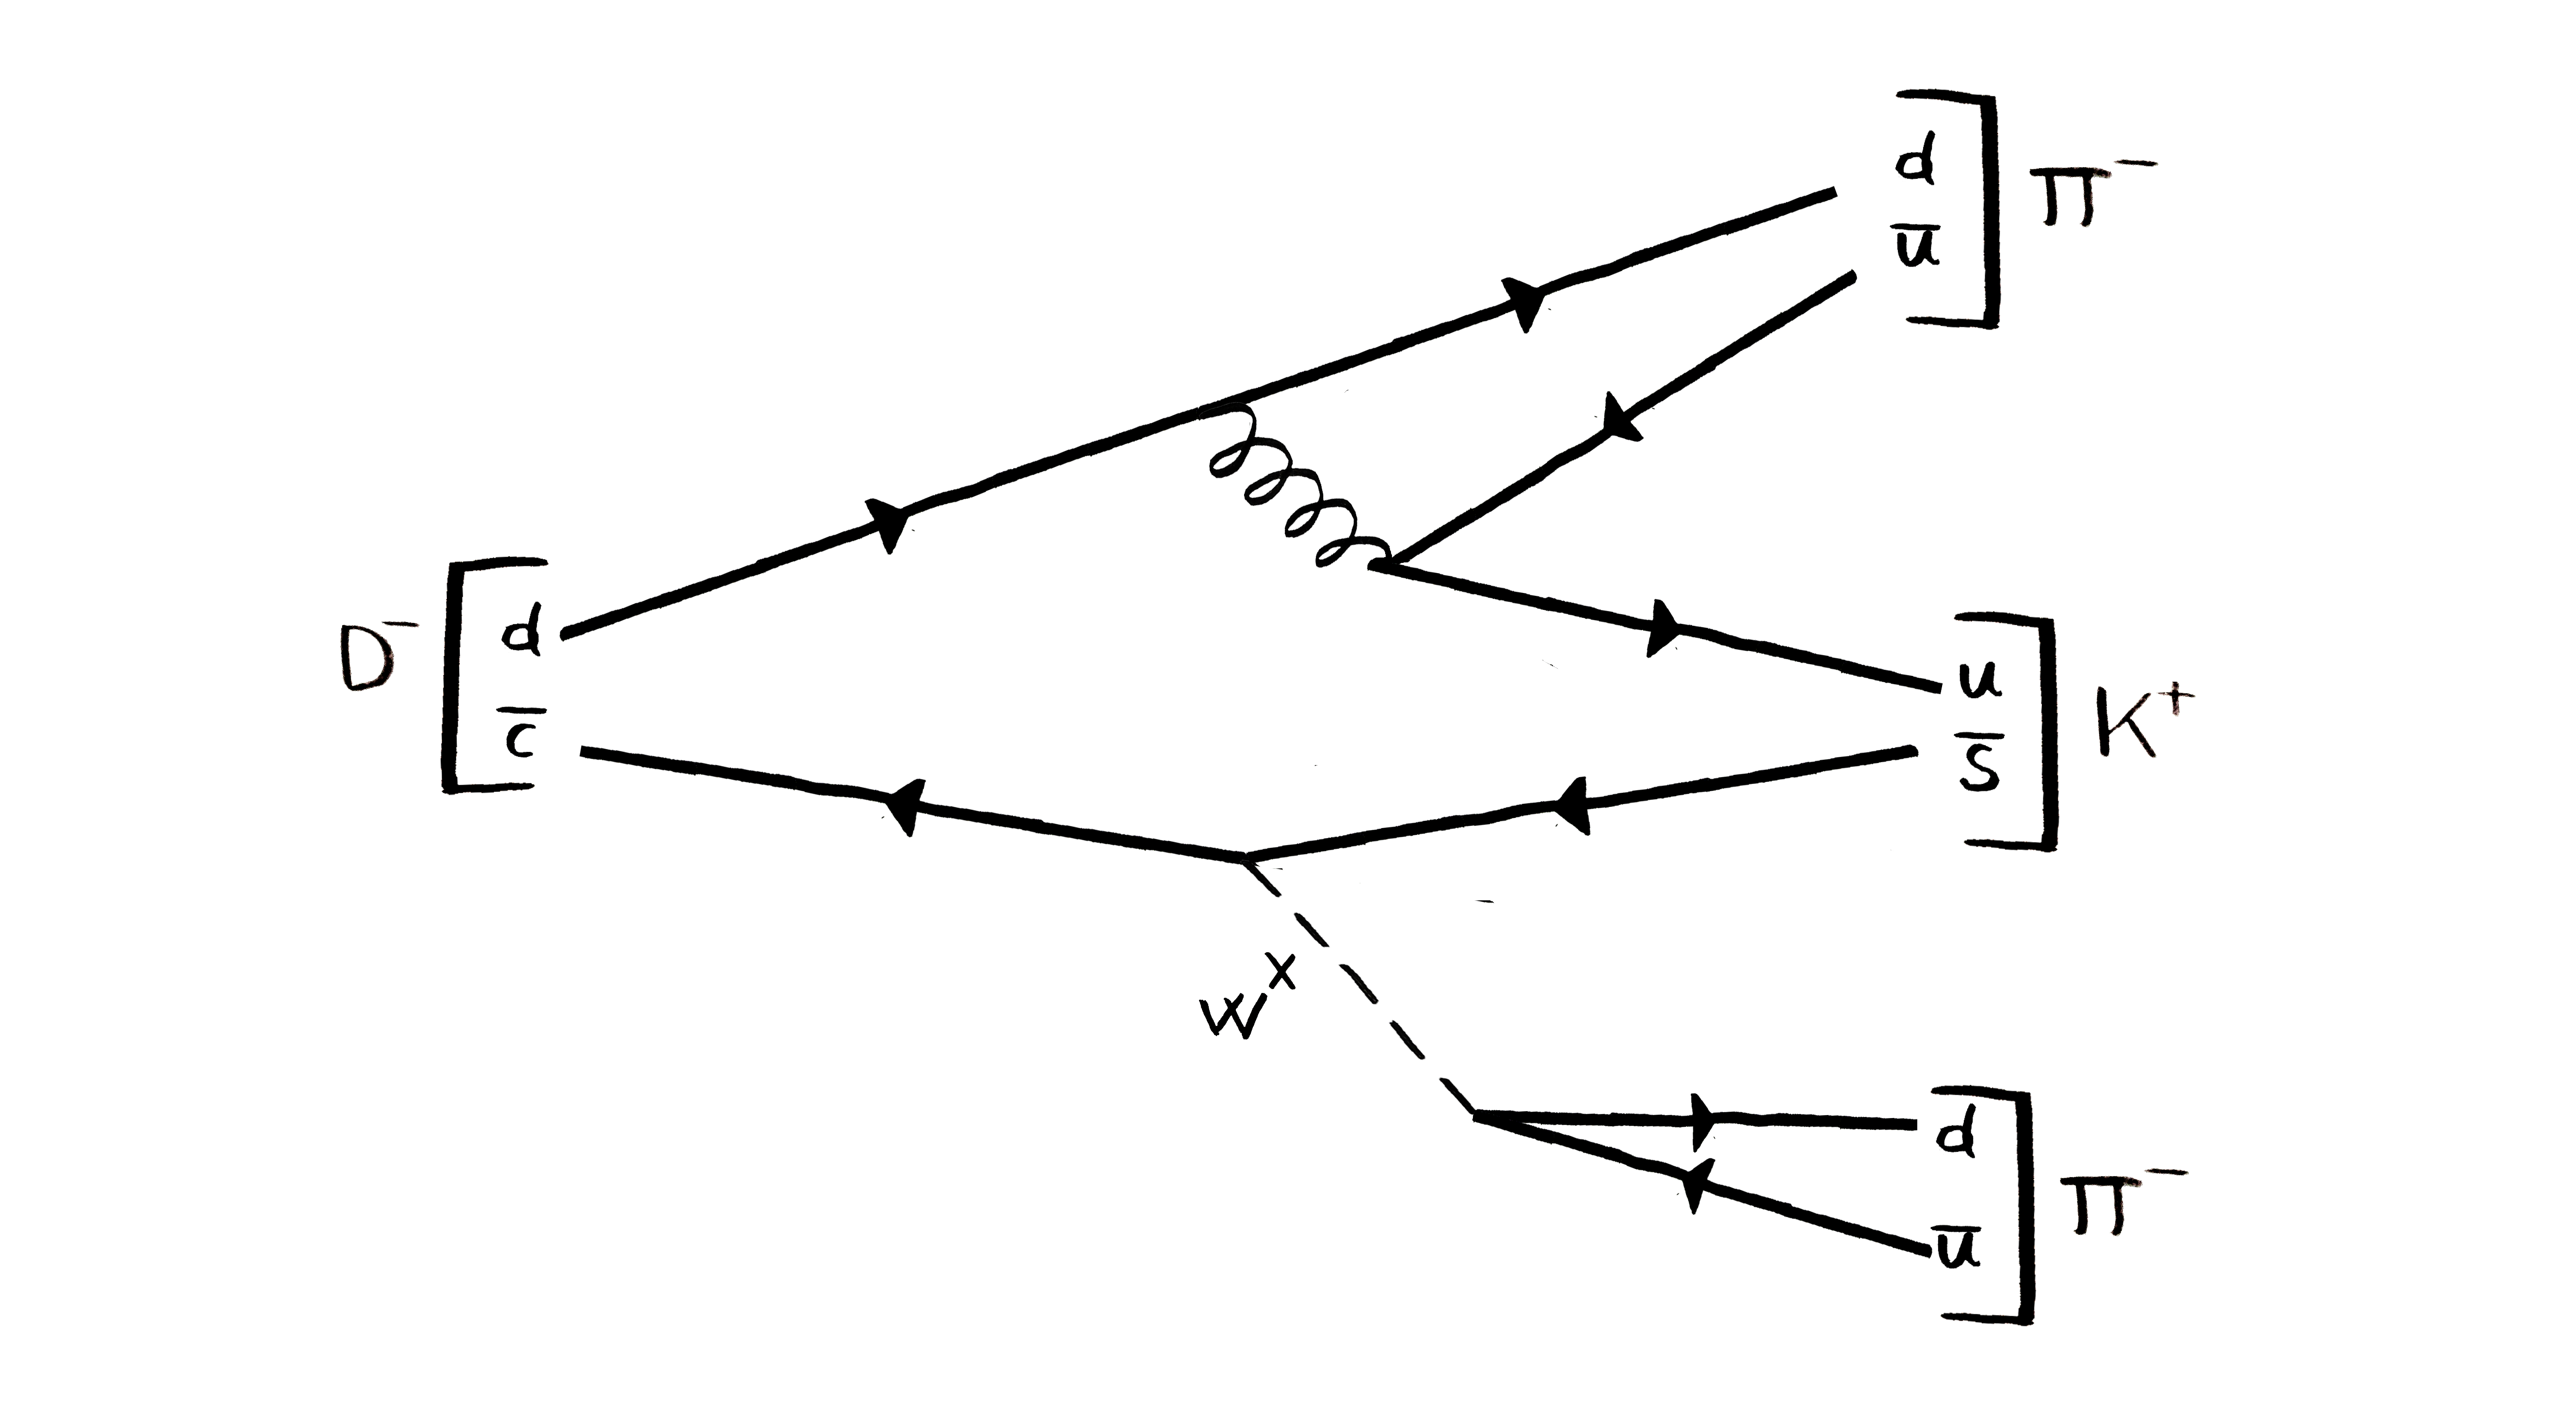
\includegraphics[width=0.8\textwidth]{KernePartikel/reaction3.png}
  \caption{Henfaldet af $D^-$.}
  \label{fig:D_reaction}
\end{figure}
Udfordringen består i at lave et feynman-diagram som er så overskueligt som muligt (f.eks. uden krydsende pile) og som gør brug af \emph{mindst mulige vertexer og derved virtuelle partikler}. Fysisk set betyder færre vertexer = større sandsynlighed.
\opg Hvad er ladningen af $W$-bosonen i figur \ref{fig:D_reaction}?
\opg Beskriv med ord hvad der sker med hver af kvarkerne i $D^-$-mesonen.
\opg Prøv at lave et feynman-diagram for henfaldet: $D^- \rightarrow K^- + \pi^+ + \pi^-$. \emph{Hint: start med at finde kvarksammensætningen af partiklerne.}
\end{opgave}

\begin{opgave}{Relativistiske partikler}{2}
Partikelacceleratorer gør brug af, at partikler kan opnå kæmpe energi ved at blive accelereret op i nærheden af lysets hastighed $c$. Hvis en observatør målte massen af en partikel med hastigheden $v$, ville han måle en større masse end den masse partiklen har, hvis den er i hvile. Man kan vise, at den masse som observatøren måler (kaldet den relativistiske masse, $m_\text{rel}$) er relateret til partiklens hvilemasse $m$ og hastighed $v$ gennem:
\begin{equation}
m_\text{rel} = \frac{m}{\sqrt{1-v^2/c^2}}
\end{equation}
\opg I en bestemt accelerator accelereres elektroner ($m=0,511\SI{}{Mev/c^2}$) op sådan at deres energi bliver $E=580$Mev. Brug $E=m_\text{rel}c^2$ til at finde elektronernes hastighed i enheder af lysets hastighed $c$.
\opg Hvad er elektronernes relativistiske masse?
\end{opgave}

\begin{opgave}{Flere feynman-diagrammer}{2}
\emph{NB: det er en god idé at du har lavet opgave \ref{opg:feynman1} inden denne opgave.}

Tegn feynman-diagrammer for følgende henfald. Husk at gøre brug af mindst mulige vertexer.
\opg $B^- (b\bar{u}) \longrightarrow D^0(c\bar{u}) + \rho^-(d\bar{u})$
\opg $\Sigma^-(dds) \longrightarrow \Lambda^0 (uds) + e^- + \bar{\nu}_e$
\opg $\Delta^0 (udd) \longrightarrow p + \pi^- (d\bar{u})$
\opg $D_s^+ (c\bar{s}) \longrightarrow \phi (s\bar{s}) + \rho^+ (u\bar{d})$
\opg $\Omega^-(sss) \longrightarrow \Xi^-(dss) + \pi^0(u\bar{u})$
\end{opgave}

\chapter{Kerne-- og Partikelfysik Facitliste}
\section*{Kernefysik}
\begin{opgave}{Alfa-henfald}{1}
\begin{equation*}
^{238}_{92} \text{U} \rightarrow ^{234}_{90}\text{Th} + ^{4}_{2}\text{He}.
\end{equation*}
\opg Alfa-partiklen har både magiske tal $Z=2$ og $N=2$, og er derfor utroligt stabil. Det er særligt energimæssigt favorabelt at henfalde til en kerne og en alfa-partikel end f.eks. to arbitrære kerner.
\opg Reaktionens $Q$-værdi udregnes som $Q=(M_i - M_f)c^2$. Her er $M_i=M(^{238}_{92} \text{U})$ og $M_f=M(^{232}_{90}\text{Th}+M(^{4}_{2}\text{He}))$. Med masserne opgivet i atomare masse-enheder anvendes det, at der omregnes til energi gennem $1 u = 931,49406\SI{}{MeV/c^2}$. Dette giver:
\begin{equation*}
Q = 4,273695~\SI{}{MeV}
\end{equation*}
$Q$-værdien er positiv, så reaktionen kan forekomme naturligt.
\end{opgave}

\begin{opgave}{Berylliums isotoper}{2}
\opg Den atomare masse af Be-8 sammenlignes med massen af to He-4.  Be-8 er tungere end to He-4 med:
\begin{align*}
\Delta m &= 8,005305~\SI{}{u} - 2\cdot 4,002602~\SI{}{u}  \\
&=1,01 \cdot 10^{-4}\SI{}{u}
\end{align*}
og det er derfor energimæssigt favorabelt for Be-8 at opsplitte i to He-4.\\
\textbf{Evaluering:} Det er også det der observeres eksperimentelt. Processen udløser $0,0941~\SI{}{MeV/c^2}$ i energi.
\opg Forskellen mellem massen af Be-9 og masserne af $^7\text{Li}$ og $^2\text{H}$ er:
\begin{align*}
\Delta m &= 9,012174~\SI{}{u} - (7,016003~\SI{}{u} + 2,014102~\SI{}{u}) \\
&=-1,80 \cdot 10^{-2}~\SI{}{u}.
\end{align*}
Altså er massen af Li-7 og H-2 større end massen af Be-9.\\
Det betyder at opsplittelsen af en Be-9-kerne til en Li-7- og H-2-kerne ikke kan forekomme.\\
\textbf{Evaluering:} Isotopen Be-9 er rigtig nok stabil. 
\end{opgave}

\begin{opgave}{Kerners tæthed}{3}
Tætheden er massen delt med volumen, $\rho=\frac{m}{V}$. Volumen for en kerne, hvis den antages at være kugleformet, er $V=\frac{4}{3} \pi R^3$. Radius af en kerne er $R=R_0 A^{1/3}$. Anvendes $m\approx A$, ses det, at tætheden af en atomkerne kan siges at være:
\begin{align*}
\rho &= \frac{m}{V} \\
&\approx \frac{A}{\frac{4}{3} \pi R_0^3 A} \\
&= \frac{3}{4 \pi R_0^3}
\end{align*}
Massetallet $A$ optræder ikke ovennævnte ligning, og tætheden er derfor uafhængig af, hvilken type kerne man har med at gøre, og er derfor ens for alle kerner.
\end{opgave}

\begin{opgave}{Den stærkest bundne kerne}{1}
\label{opg:nickel}
Den energi der skal til for at splitte $^{62}\text{Ni}$ ($A=62, Z=28$ og $N=34$) er bindingsenergien, $E_B$. Den udregnes ved:
\begin{align*}
E_B &= (-\Delta M )c^2 \\
&= - (M(62,28)-28(m_p + m_e) - 34m_n)c^2 \\
&= 0,585~\SI{}{u}c^2 \\
&= 544,92~\SI{}{MeV}
\end{align*}
Det er den energi, det kræver at splitte Ni-62.
\textbf{Evaluering:} med bindingsenergien per nukleon på ca. $8,8$ er Ni-62 den stærkest bundne kerne.
\end{opgave}


\begin{opgave}{Splittelsen af en kerne}{1}
\begin{equation*}
^{28}_{14} \text{Si} + \gamma \rightarrow ^{24}_{12}\text{Mg} + X,
\end{equation*}
\opg Det ses, at $A$ for $X$ må være $28-24=4$ og $Z=14-12=2$. $X$ er derfor $^{4}_{2} \text{He}$.
\opg Hvis vi antager at energien af fotonen ikke går til kinetisk energi for $^{24}_{12}\text{Mg}$ og $X$, så er dens energi præcis tilsvarende masseforskellen mellem kernerne på hver side af reaktionstegnet. Vi kender massen af et He-atom til at være $4,002602~\SI{}{u}$, mens de andre masser er givet. Energien af fotonen må være:
\begin{align*}
E_\gamma &= (M(24,12)+M(4,2)-M(28,14))c^2 \\
&=0,011~\si{u}c^2 \\
&=10,25~\si{MeV}
\end{align*}
.
\end{opgave}


\begin{opgave}{Fusion i Solen}{2}
\begin{equation*}
4p \rightarrow \alpha + 2e^+ + 2\nu_e + E,
\end{equation*}
Dvs. der bliver desuden dannet to positroner og 2 elektronneutrinoer samt en mængde energi.
\opg Som overslag kan bruges, at massen af en alfa-partikel + massen af to positroner er den atomare masse af He-4, $M(4,2)=4,002602~\SI{}{u}$. Den energi der dannes er $Q$-værdien:
\begin{align*}
Q &= E_i - E_f \\
&= (4m_p - 4,002602~\SI{}{u})c^2 \\
&= 24,7 ~\si{MeV}.
\end{align*}
Ovenstående svar er godtaget. Men hvis man har kendskab til annihilation skal man medtage, at de to positroner vil annihilere med elektronerne i plasmaet. Dette giver (minimum) energien svarende til 4 gange elektronens hvilemasse (idet $2e^+ + 2e^- \rightarrow \gamma$). Dette giver ekstra $2~\si{MeV}$.
\opg For at få enhederne til at stemme skal ladningerne af protonerne angives i coloumb, $1e = 1,60217 \cdot 10^{-19}~\si{C}$ Den minimale energi krævet af protonerne er givet ved:
\begin{align*}
U &= \frac{1}{4\pi\epsilon_0} \frac{q_1q_2}{r} \\
&= \frac{1}{4\pi\epsilon_0} \frac{\left( 1,602 176565 \cdot 10^{-19}~\si{C}\right)^2}{1,4 \cdot 10^{-15}~\si{m}} \\
&= 1,648 \cdot 10^{-13}~\si{J}
\end{align*}
Svaret kan angives i både eV eller J, men vi skal bruge størrelsen i J i næste opgave.
\opg Energien fundet i foregående opgave indsættes i formlen:
\begin{equation*}
E = \frac{3}{2} k T.
\end{equation*}
Temperaturen findes ved:
\begin{align*}
T &= \frac{2}{3} \frac{E}{k} \\
&\approx 8 \cdot 10^9 ~\si{K}.
\end{align*}
Det er temperaturen det kræver før protonerne besidder energien fundet i foregående opgave.
Solens kernetemperatur er ca. $1,5 \cdot 10^7$K - altså meget lavere end den temperatur vi har fundet!

\textbf{Evaluering:} Fusionen af to protoner finder alligevel sted i Solens indre, til trods for den "lave" temperatur. Temperaturen af protonerne følger en fordeling, som topper ved temperaturen $1,5 \cdot 10^7$K. Det betyder at størstedelen af protonerne har denne temperatur. Men det er muligt for protonerne at have både højere og lavere temperaturer end dette - derfor kan fusionen foregå. Det sker bare med meget lavere sandsynlighed. Det er bl.a. det der afgør hvorfor stjerner som Solen har lang levetid!
\opg Solkonstanten er energi i joule der rammer hver kvadratmeter af Jordens overflade per sekund. Omregning fra joule til MeV:
\begin{align*}
\si{J} &= \frac{1}{1,60217 \cdot 10^{-19}} \si{eV} \\
&= \frac{1}{1,60217 \cdot 10^{-19}} \si{eV} \cdot 10^{-6}~\si{MeV/eV} 
\end{align*} 
Vi starter med at omregne til kvadratcentimeter og MeV:
\begin{align*}
S_0 &=1,362 \cdot 10^3~\SI{}{J m^{-2} s^{-1}} \\
&=1,362 \cdot 10^7~\SI{}{J cm^{-2} s^{-1}} \\
&= 1,362 \cdot 10^7~\SI{}{J cm^{-2} s^{-1}} \cdot \frac{1}{1,60217 \cdot 10^{-19}} \si{eV/J} \cdot 10^{-6}~\si{MeV/eV} \\
&\approx 8,5 \cdot 10^{19}~\SI{}{MeV cm^{-2} s^{-1}}
\end{align*}
Hvis al energi fra Solen dannes af ovenstående reaktion, forekommer der $S_0/E$ reaktioner per sekund, hvor $E$ er energien udløst i reaktionen regnet i foregående opgave. Der dannes to neutrinoer per reaktion, så fluxen af neutrioner per kvadratcentimeter per sekund på Jordens overflade er:
\begin{align*}
\Phi_\nu &=2 \frac{S_0}{E} \\
&=2 \frac{8,5 \cdot 10^{19}~\SI{}{MeV cm^{-2} s^{-1}}}{24,7~\SI{}{MeV}} \\
&\approx 7 \cdot 10^{18}~\SI{}{cm^{-2} s^{-1}}
\end{align*}
En fingerspids har ca. areal på $1~\SI{}{cm^2}$. Antal neutrinoer som rammer en fingerspids per sekund er da:
\begin{align*}
\text{antal:} &= \Phi/\text{areal} \\
&\approx 7 \cdot 10^{18}~\SI{}{s^{-1}}
\end{align*}
\textbf{Evaluering:} Dette tal er stærkt overvurderet idet vi antog, at \emph{al} Solens energi blev båret væk af neutrinoer.
\end{opgave}

\begin{opgave}{Dannelse af tunge grundstoffer i en supernova: r- og s-proces}{2}
\opg I kernen fusioneres lettere elementer til tungere. Dette skaber løgstruktur i stjernen med lette elementer yderst og tunge elementer inderst. Bindingsenergien for jern er så høj, at stjernen ikke vinder energi ved at omdanne lettere grundstoffer til jern. Derfor stopper fusionen, når stjernen har opnået en jern-kerne.
\opg Hvis en kerne fanger én neutron, ændrer $N$ sig med +1. Det svarer til at tage ét skridt til højre på kernekortet. Hvis kernen undergår beta-minus-henfald, så falder $N$ med 1 og $Z$ stiger med 1. Det svarer til at tage ét skridt skråt tilbage på kernekortet.
\opg Ved fem r-proces neutronindfangninger svarer det til at gå fem skridt mod højre på kernekortet. Her ender man ved kernen 186-Ta. Herefter henfalder kernen ved beta-minus indtil den når en stabil kerne, dvs. man går skråt tilbage på kernekortet til man rammer en sort firkant. Man ender ved 186-W.
\opg Ved fem s-proces skal der tages et skridt skråt tilbage efter hvert skridt til højre, hvis kernen er ustabil. Her ender man ved 186-Os.
\opg Kernen 180-Ta kan ikke dannes ved neutronindfangning, da den befinder sig på den anden side af stabilitetslinjen.
\end{opgave}

\newpage
\section*{Partikelfysik}

\begin{opgave}{Bevarelseslove}{1}
\opg Følgende bevarelseslove gør sig gældende:
\begin{itemize}
\item Lepton-tal
\item Baryon-tal
\item Energi
\item Impuls
\item Ladning
\end{itemize}
For at tjekke om en reaktion kan lade sig gøre, tjekkes der for bevarelse af lepton-tal, baryon-tal og ladningsbevarelse.
\opg
\begin{enumerate}
\item $e^- \longleftrightarrow e^- + e^+ + e^+$ (ikke tilladt, ladning og lepton-tal)
\item $p + n \longleftrightarrow e^- + e^+ + e^+$ (ikke tilladt, baryon-tal og lepton-tal)
\item $p + n + e^+ \longleftrightarrow n + p + \bar{\nu}_e$ (ikke tilladt, ladning)
\item $p \longleftrightarrow \mu^- + n + \bar{\nu}_\mu $ (ikke tilladt, ladning)
\item $p \longleftrightarrow \mu^+ + n + \nu_\mu $ (tilladt)
\item $\bar{n} \longleftrightarrow \bar{p} + e^+ + \nu_e$ (tilladt)
\item $e^- + \mu^+ \longleftrightarrow n$ (ikke tilladt, baryon-tal og lepton-tal)
\end{enumerate}
.
\end{opgave}

\begin{opgave}{Dannelse af to muoner}{1}
Feynman-diagram, hvor en foton danner muoner i en pardannelsesproces:
\begin{figure}[h]
  \centering
  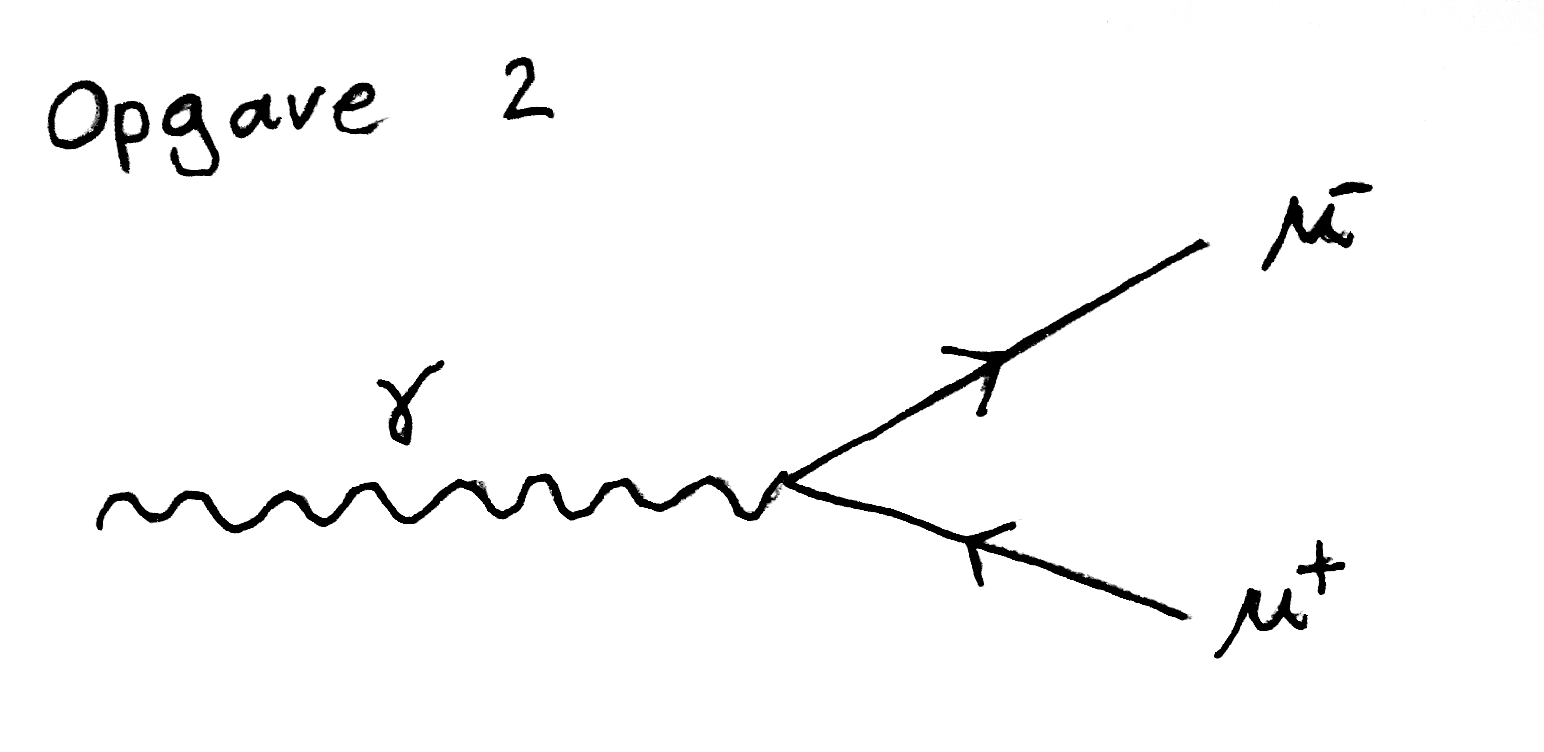
\includegraphics[width=0.4\textwidth]{KernePartikel/opg2.png}
  \caption{Muon pardannelse}
  \label{fig:opg2}
\end{figure}
En muon har hvilemassen $105,7$ \si{MeV/c^2}. Energien for at danne et par er derfor givet ved:
\begin{align*}
E &= 2 m_{\mu} c^2 \\
&= 211,4~\si{MeV} = 3,38~ 10^{-17} \si{J}
\end{align*}
\end{opgave}

\begin{opgave}{Reaktioner med $W^\pm$-partiklen}{2}
\label{opg:W}
\opg
\begin{figure}[h]
  \centering
  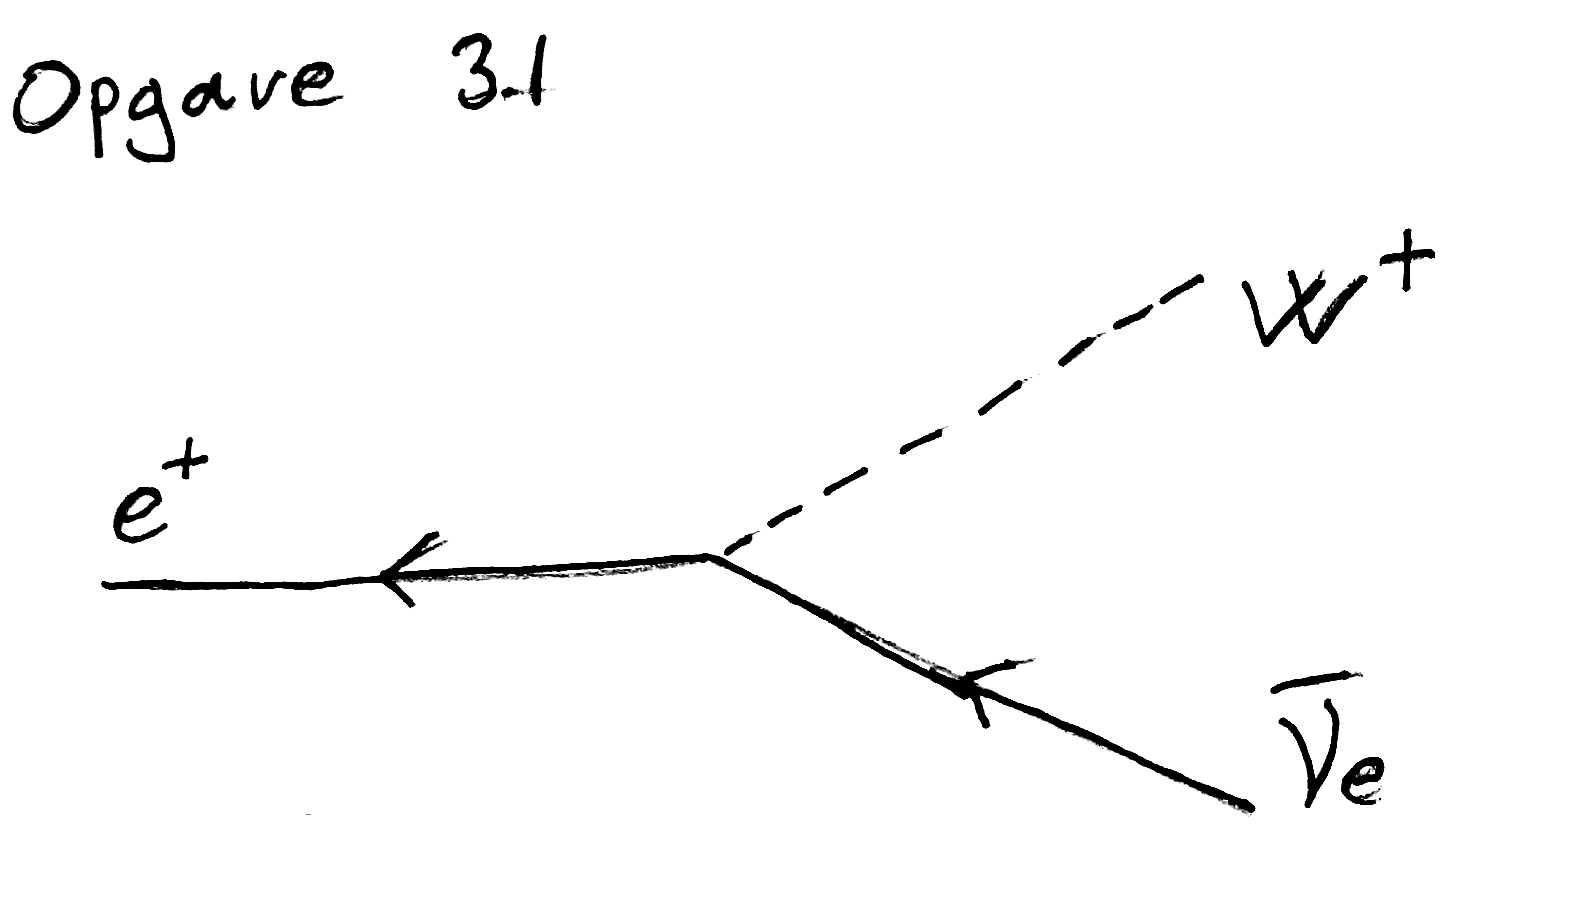
\includegraphics[width=0.4\textwidth]{KernePartikel/opg31.png}
  \caption{Rotation af Feynmandiagram.}
  \label{fig:opg31}
\end{figure}
Se figur \ref{fig:opg31}.
\bigskip
Elektronen bliver til en positron og elektronneutrinoen bliver til en anti-elektronneutrino.
\opg
\begin{figure}[h]
  \centering
  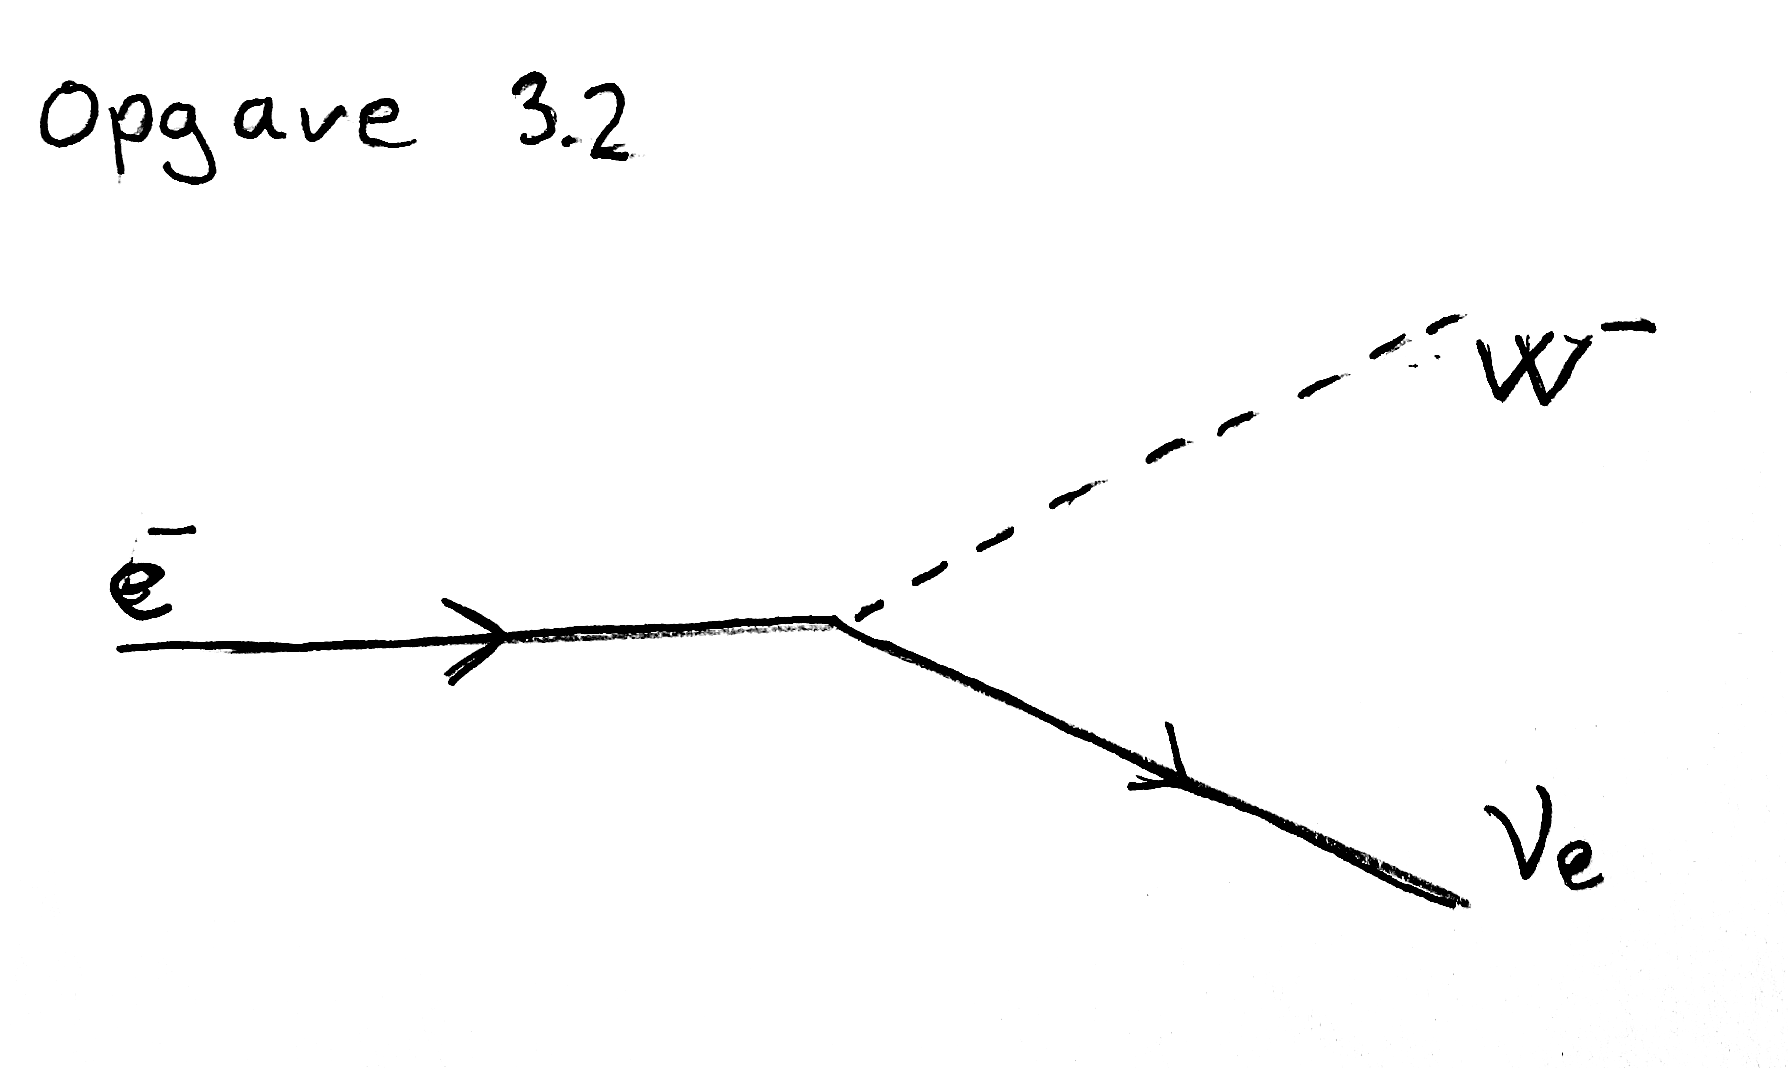
\includegraphics[width=0.4\textwidth]{KernePartikel/opg32.png}
  \caption{Elektron i stedet for positron som indgang.}
  \label{fig:opg32}
\end{figure}
Se figur \ref{fig:opg32}.
\bigskip
Positronen bliver til en electron og anti-elektronneutrinoen bliver til en elektronneutrino.
\opg Feynman-diagrammet for et beta-plus-henfald: $p \rightarrow
n + e^+ + \nu_e$.
\begin{figure}[h]
  \centering
  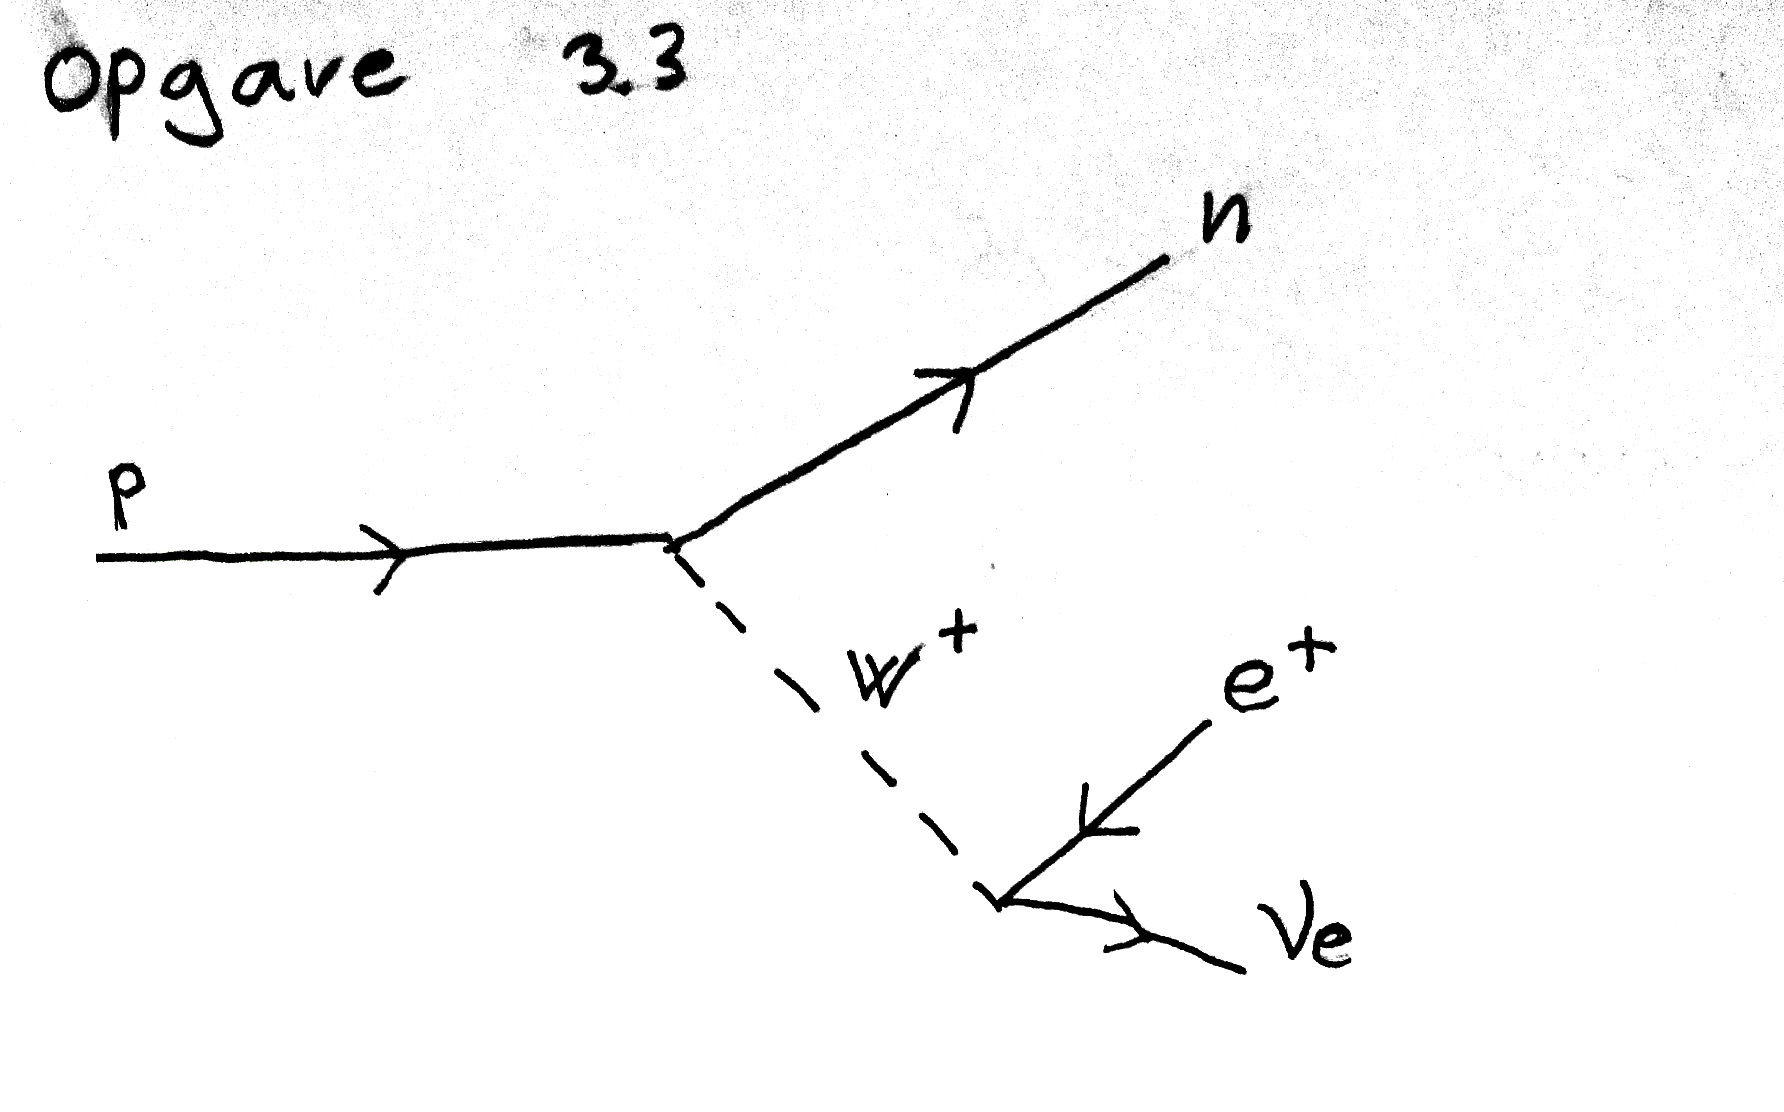
\includegraphics[width=0.4\textwidth]{KernePartikel/opg33.png}
  \caption{Beta plus henfald}
  \label{fig:opg33}
\end{figure}
Se figur \ref{fig:opg33}.
\bigskip
Protonen bliver til en neutron under udsendelse af en $W^+$-partikel, der henfalder til et positron-elektronneutrino-par.
\opg Tegn feynman-diagrammet for en elektron-indfangning: $p + e^-
\rightarrow n + \nu_e$.
\begin{figure}[h]
  \centering
  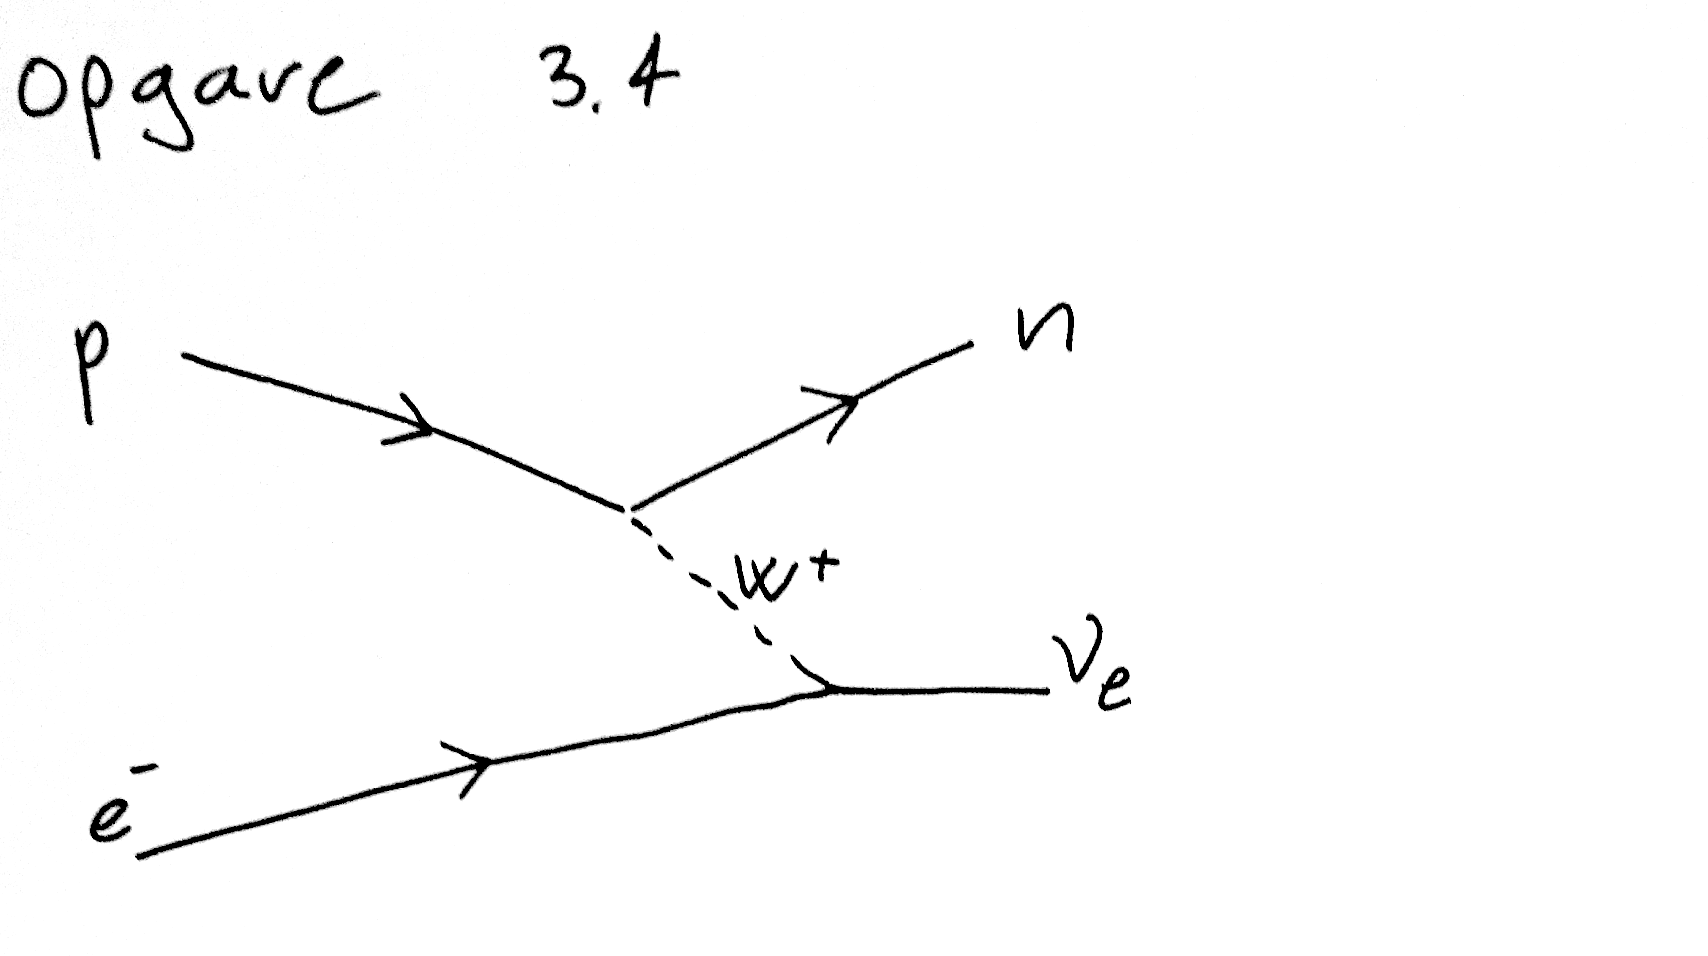
\includegraphics[width=0.4\textwidth]{KernePartikel/opg34.png}
  \caption{Elektron-indfangning}
  \label{fig:opg34}
\end{figure}
Se figur \ref{fig:opg34}.
\bigskip
Processen sker i to trin: udsendelsen af en W-boson fra protonen under omdannelse til en neutron. W-bosonen kan møde elektronen og danne en elektron-neutrino.
\opg Indtegn på figur \ref{fig:Wquarks} pile mellem alle de kvarker, som $W$ kan omdanne. 
\begin{figure}[h]
  \centering
  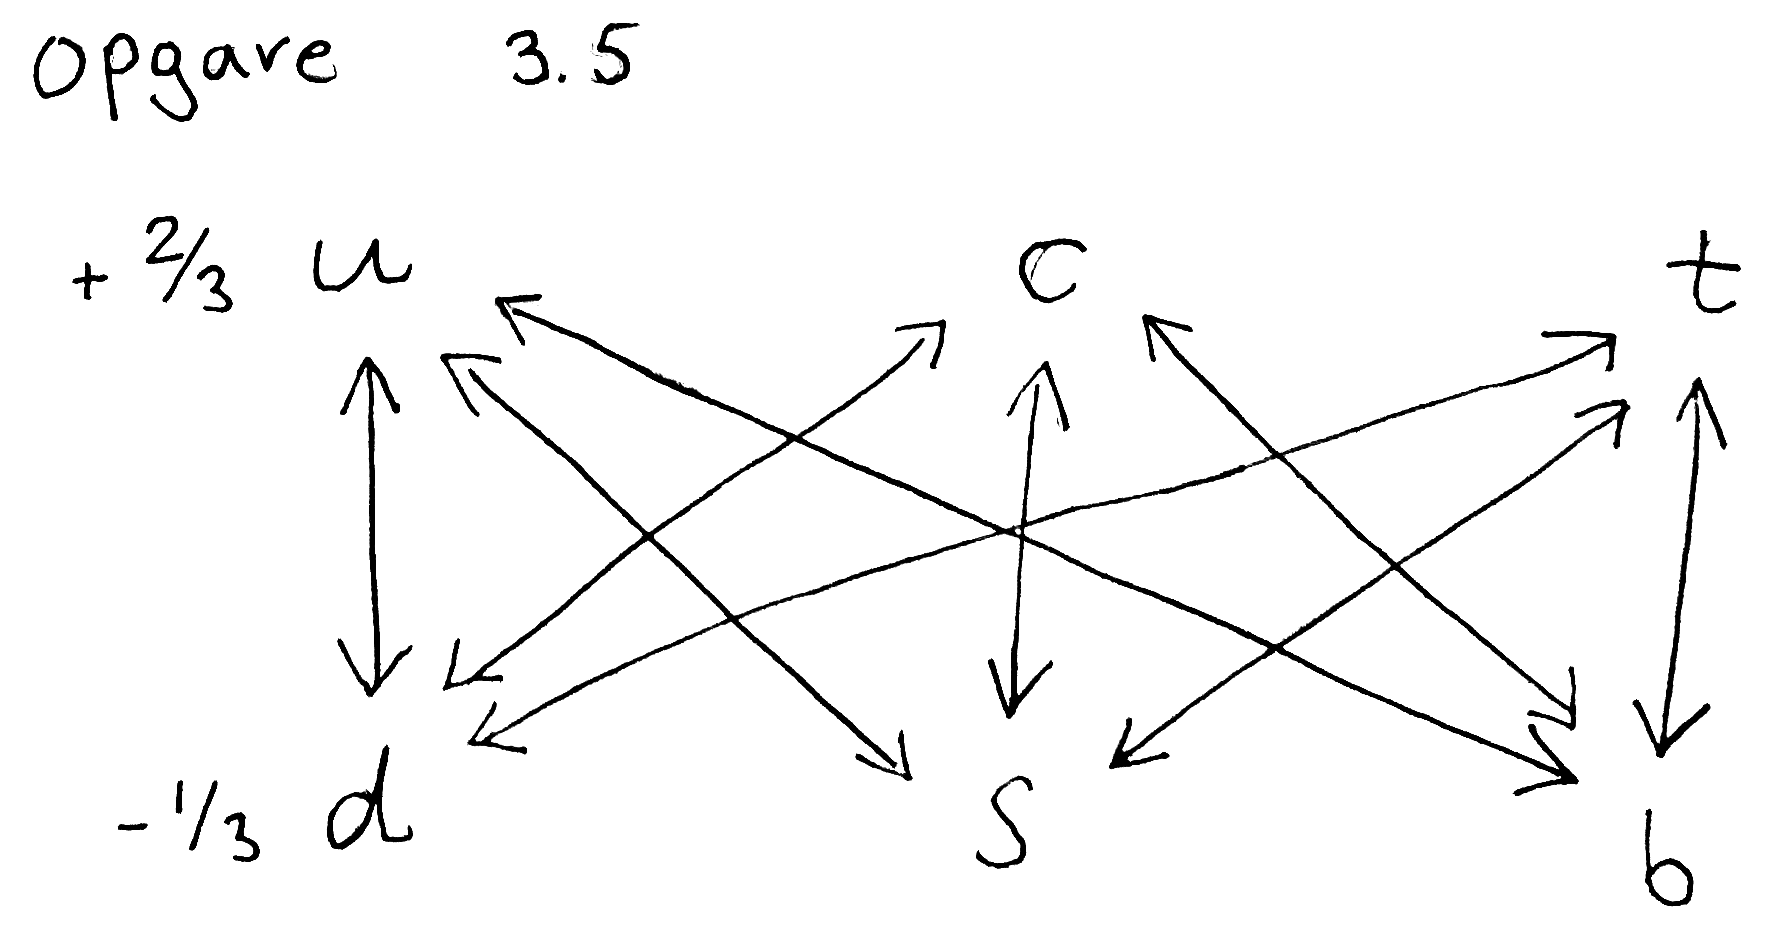
\includegraphics[width=0.4\textwidth]{KernePartikel/opg35.png}
  \caption{Kvarkomdannelser, som $W$ kan lave.}
  \label{fig:opg35}
\end{figure}
Se figur \ref{fig:opg35}.
\opg 
\begin{figure}[h]
  \centering
  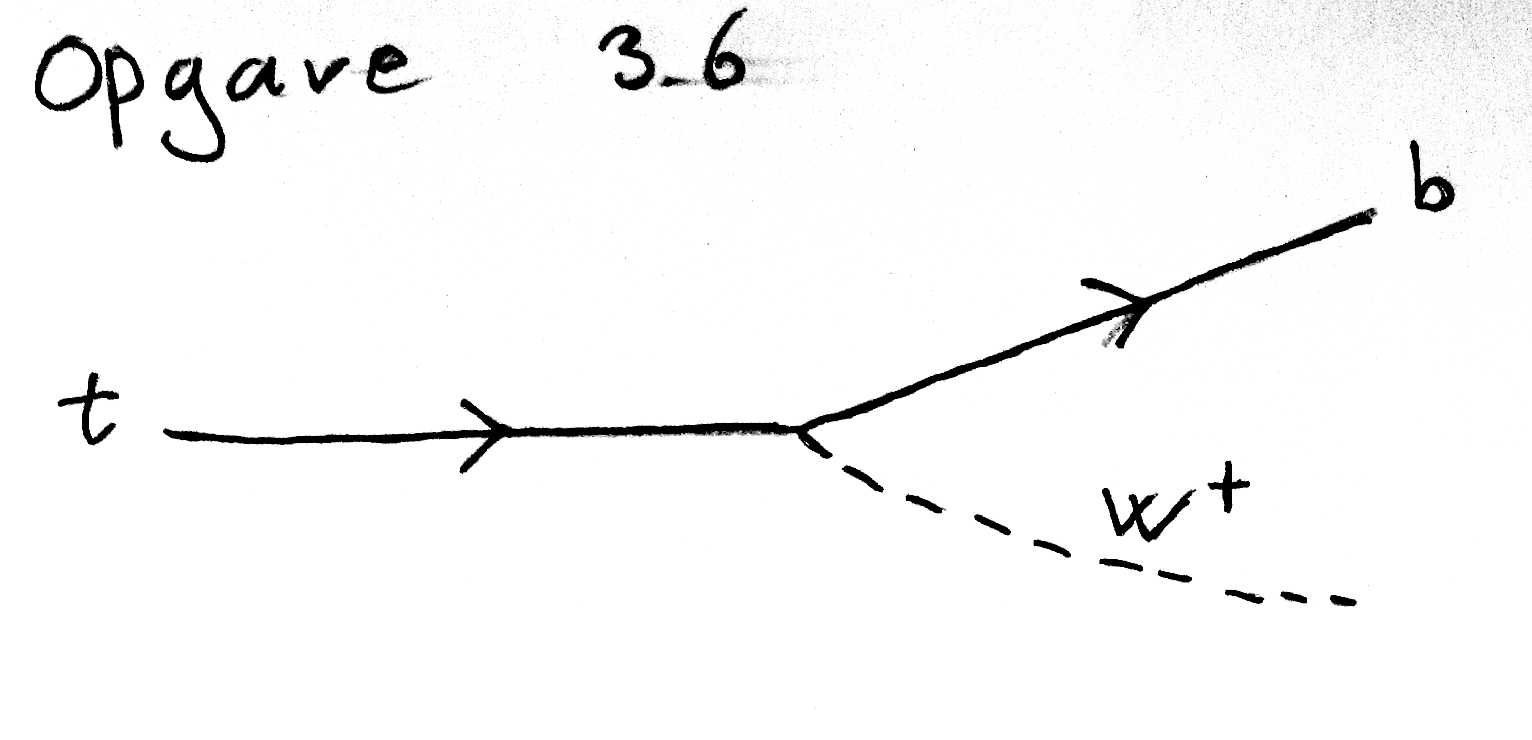
\includegraphics[width=0.4\textwidth]{KernePartikel/opg36.png}
  \caption{t-kvark omdannes til b-kvark.}
  \label{fig:opg36}
\end{figure}
Se figur \ref{fig:opg36}.
\bigskip
Ladningen af $W$ er +1.
\opg 
\begin{figure}[h]
  \centering
  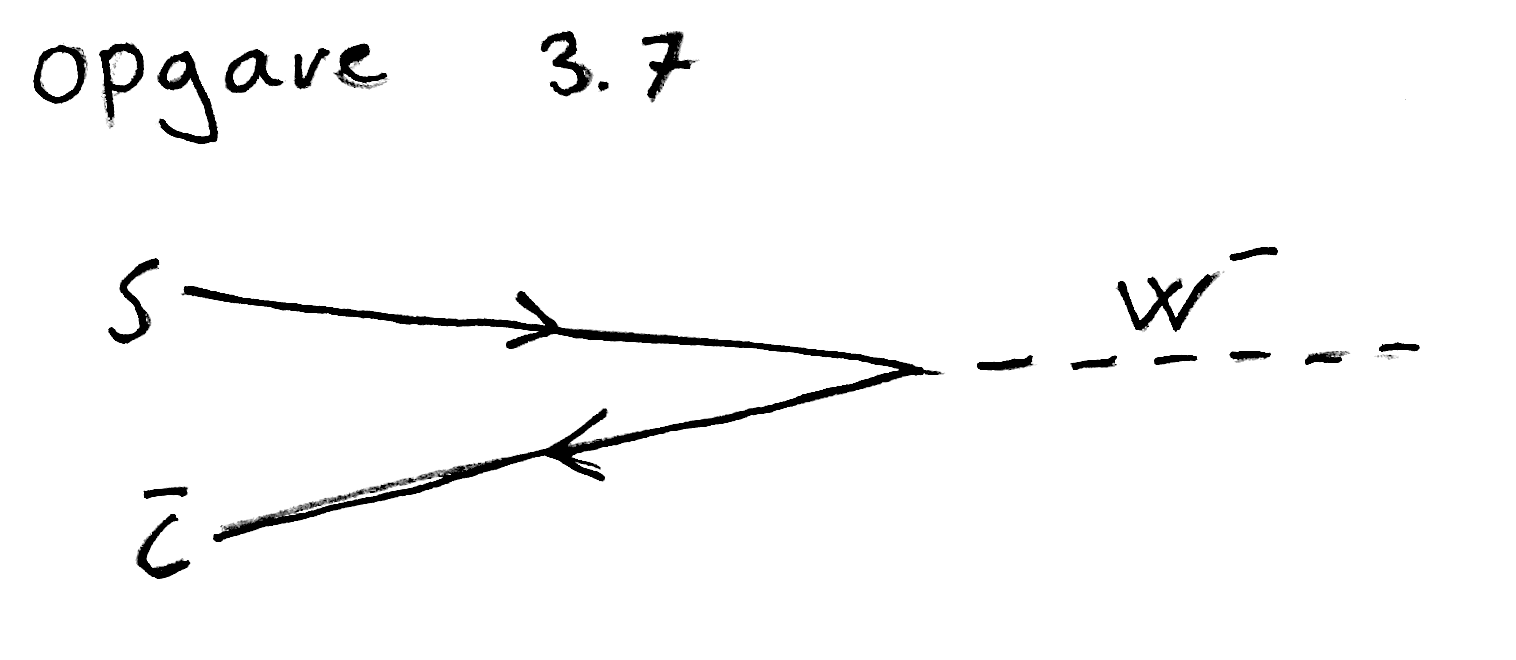
\includegraphics[width=0.4\textwidth]{KernePartikel/opg37.png}
  \caption{s-kvark og anti-c kvark annihilerer.}
  \label{fig:opg37}
\end{figure}
Se figur \ref{fig:opg37}.
\bigskip
Ladningen af $W$ er -1.
\opg 
\begin{figure}[h]
  \centering
  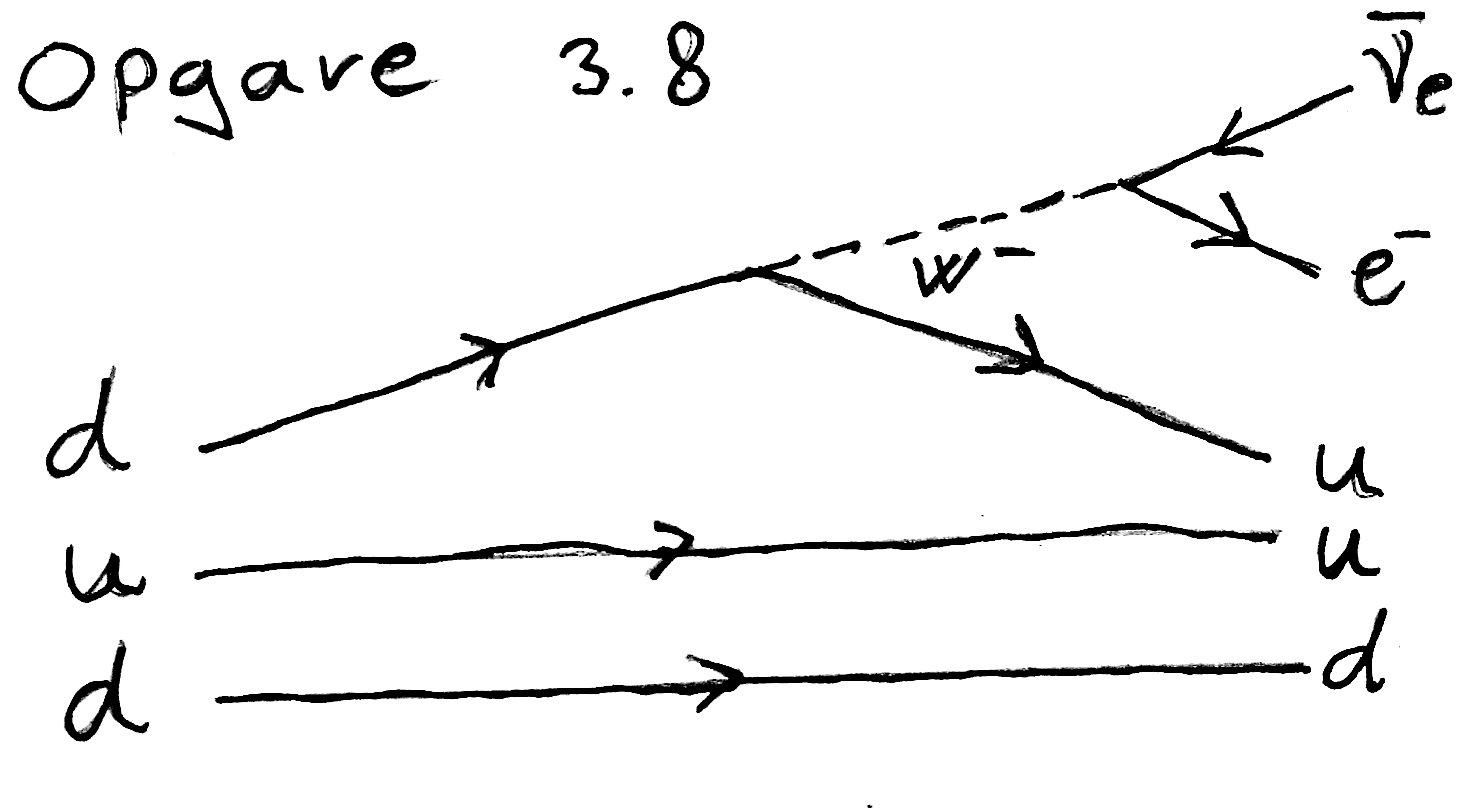
\includegraphics[width=0.4\textwidth]{KernePartikel/opg38.png}
  \caption{Beta minus henfald.}
  \label{fig:opg38}
\end{figure}
Se figur \ref{fig:opg38}.
\end{opgave}


\begin{opgave}{Feynman-diagrammer: en sand kunstart}{3}
\label{opg:feynman1}
\opg Ladningen af $W$ er -1.
\opg Den ene kvark udsender en gluon og passerer derefter uændret. Gluonen henfalder til et kvark/anti-kvark-par. Den anden kvark i $D^-$-mesonen ændres under udsendelse af en $W^-1$. Denne $W^-$ henfalder og skaber to nye kvarker.
\opg 
\begin{figure}[h]
  \centering
  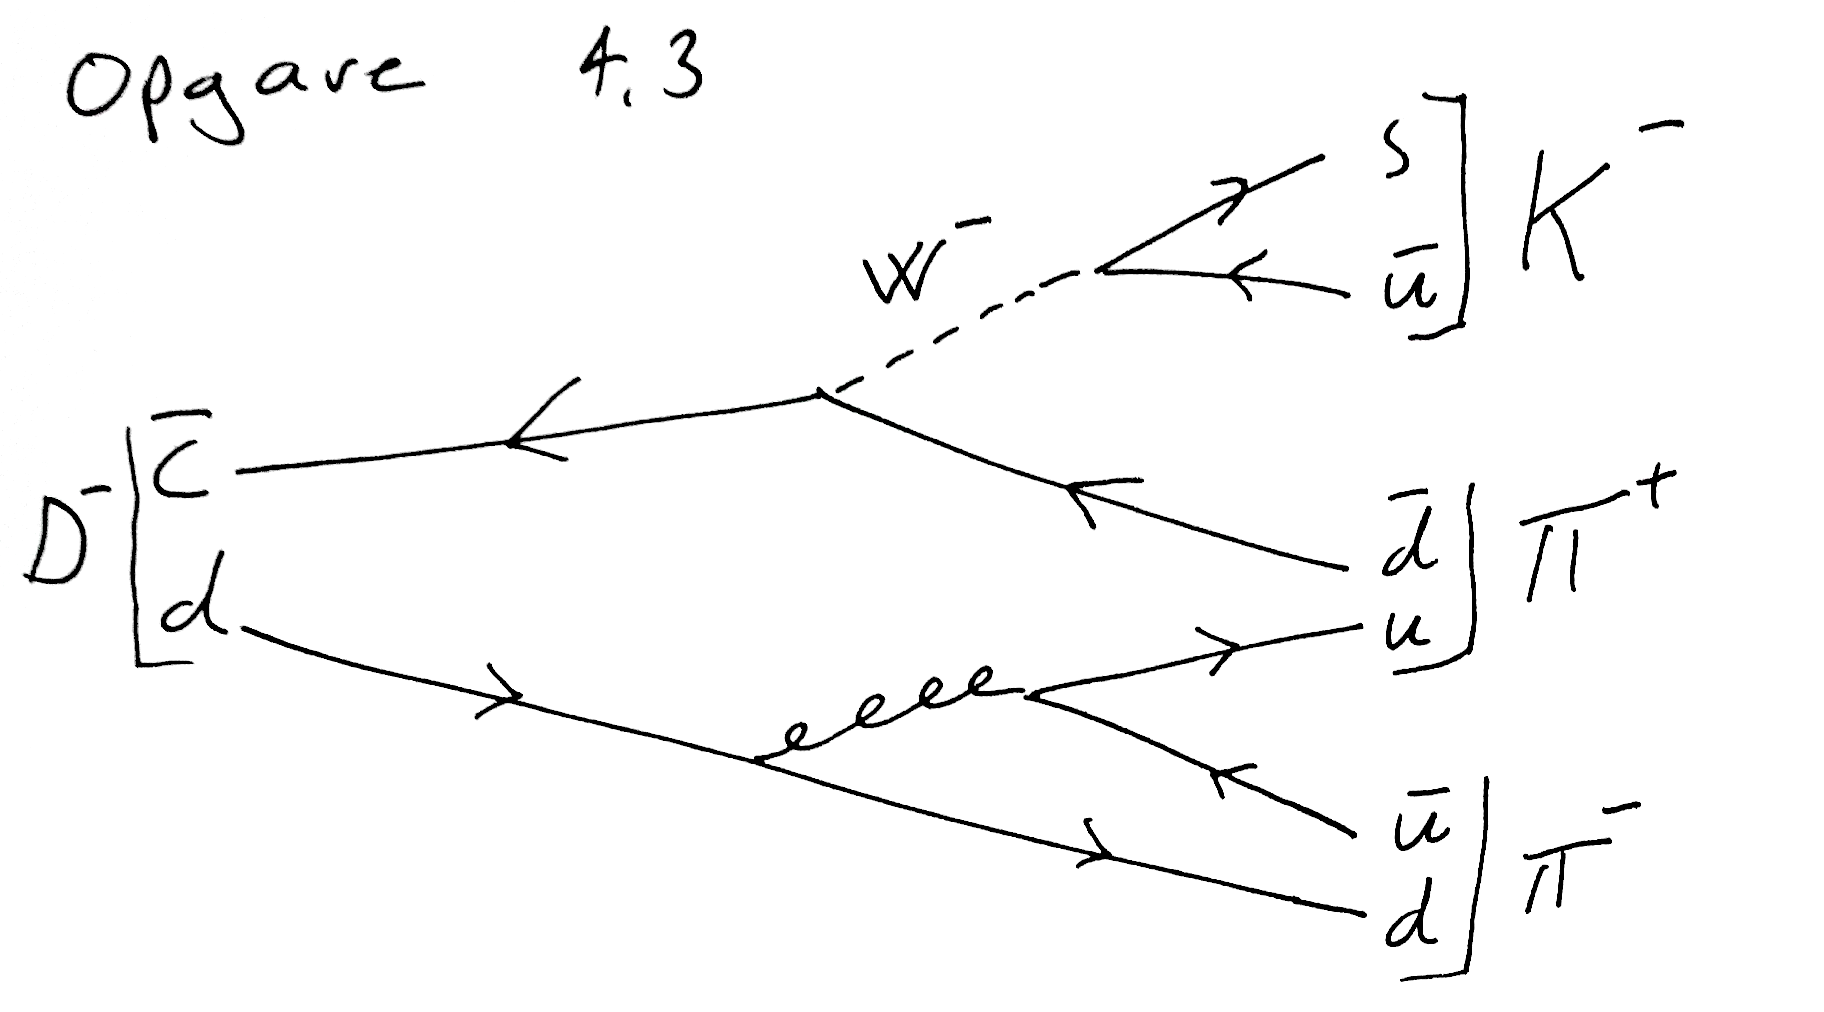
\includegraphics[width=0.4\textwidth]{KernePartikel/opg43.png}
  \caption{Feynmandiagram for henfald af $D^-$-mesonen.}
  \label{fig:opg43}
\end{figure}
Se figur \ref{fig:opg43}.
\bigskip
\end{opgave}

\begin{opgave}{Relativistiske partikler}{2}
\opg 
\begin{align*}
E & = m_\text{rel} c^2 \\
E & = \frac{m}{\sqrt{1-v^2/c^2}} c^2 \\
v/c & = \sqrt{1-\frac{m^2 c^4}{E^2}} \\
&= 0,99999961
\end{align*}
\opg Den relativistiske masse er allerede givet af opgaven gennem Einstein\'s formel $E=mc^2$:
\begin{align*}
m_\text{rel} & = 580~\si{MeV/c^2} = 1,03~ 10^{-27} ~\si{kg}
\end{align*}
\end{opgave}

\begin{opgave}{Flere feynman-diagrammer}{2}
\opg $B^- (b\bar{u}) \longrightarrow D^0(c\bar{u}) + \rho^-(d\bar{u})$
\begin{figure}[h]
  \centering
  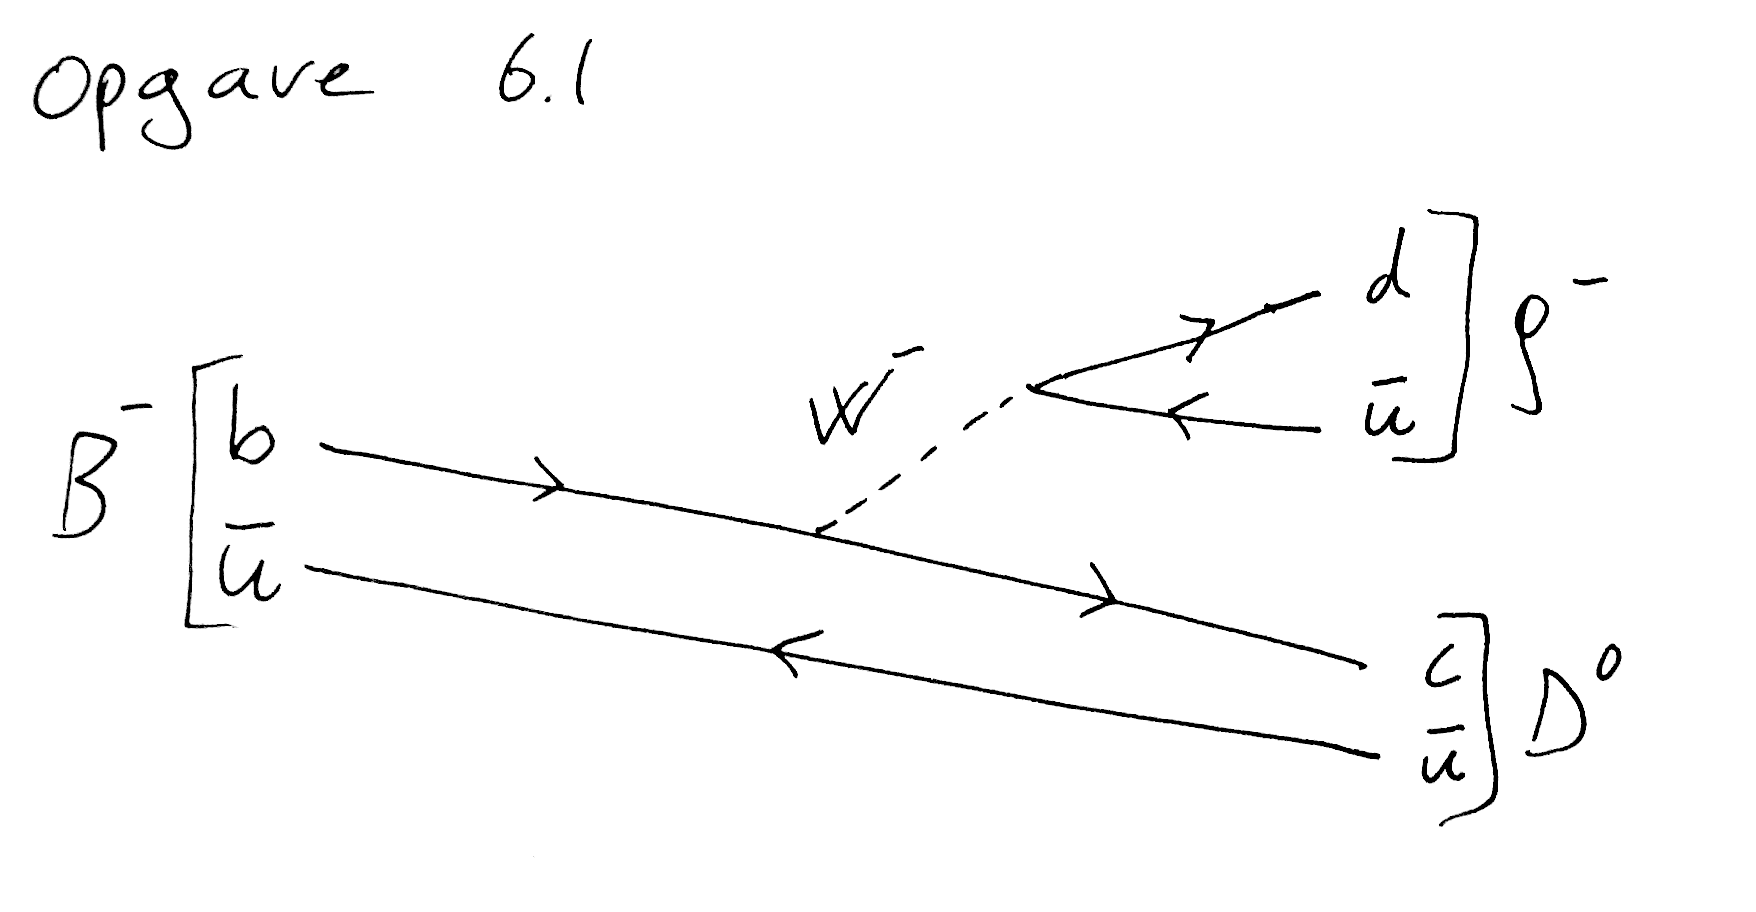
\includegraphics[width=0.4\textwidth]{KernePartikel/opg61.png}
  \caption{Feynmandiagram for henfald af $B^-$.}
  \label{fig:opg61}
\end{figure}
Se figur \ref{fig:opg61}.
\opg $\Sigma^-(dds) \longrightarrow \Lambda^0 (uds) + e^- + \bar{\nu}_e$
\begin{figure}[h]
  \centering
  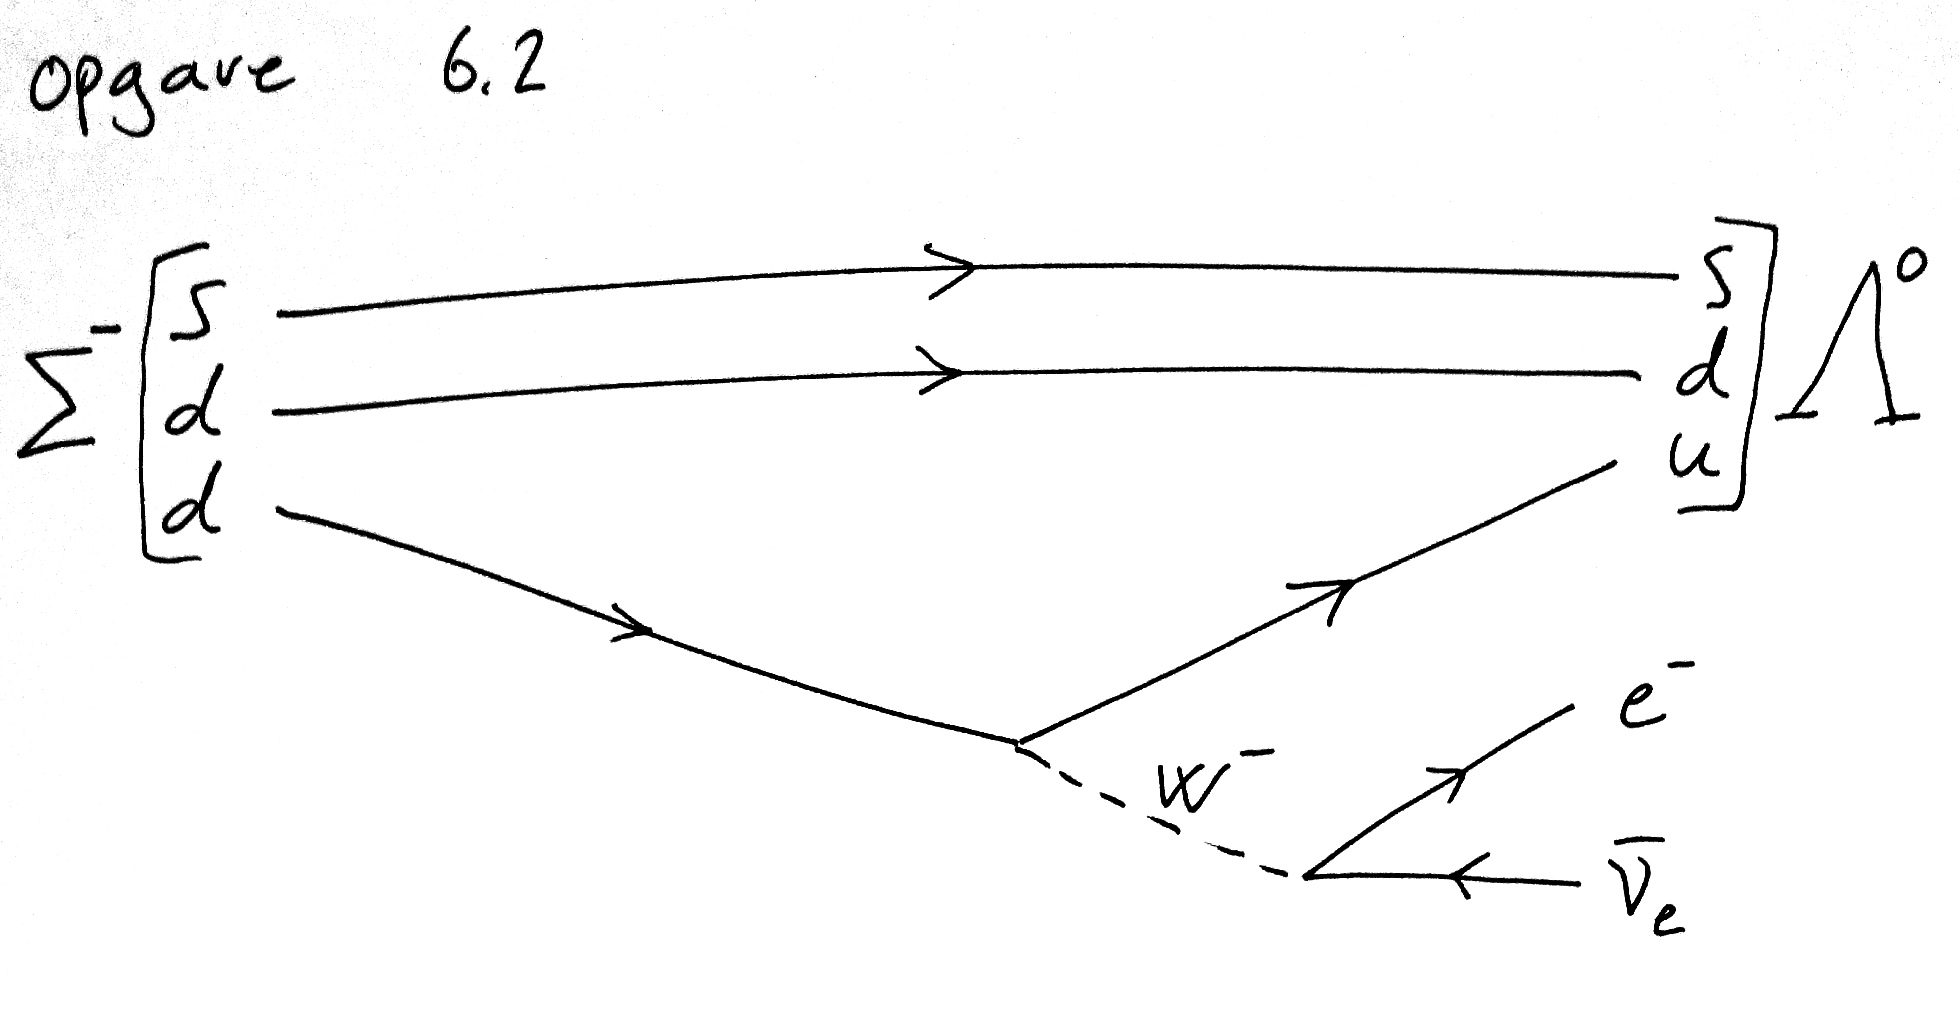
\includegraphics[width=0.4\textwidth]{KernePartikel/opg62.png}
  \caption{Feynmandiagram for henfald af $\Sigma^-$.}
  \label{fig:opg62}
\end{figure}
Se figur \ref{fig:opg62}.
\opg $\Delta^0 (udd) \longrightarrow p + \pi^- (d\bar{u})$
\begin{figure}[h]
  \centering
  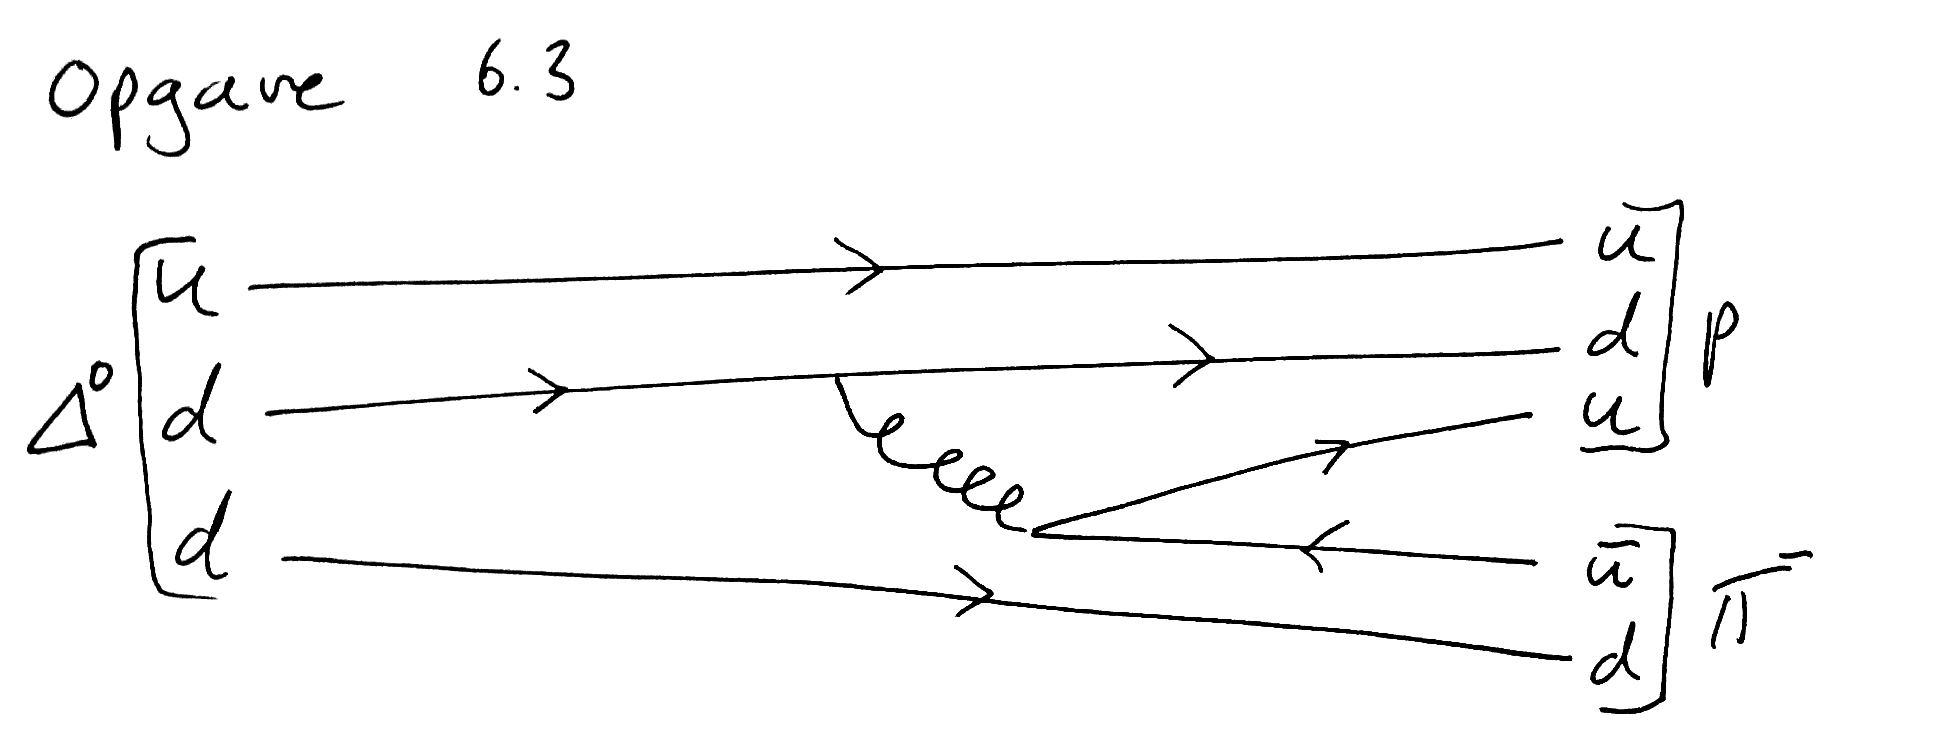
\includegraphics[width=0.4\textwidth]{KernePartikel/opg63.png}
  \caption{Feynmandiagram for henfald af $\Delta^0$.}
  \label{fig:opg63}
\end{figure}
Se figur \ref{fig:opg63}.
\opg $D_s^+ (c\bar{s}) \longrightarrow \phi (s\bar{s}) + \rho^+ (u\bar{d})$
\begin{figure}[h]
  \centering
  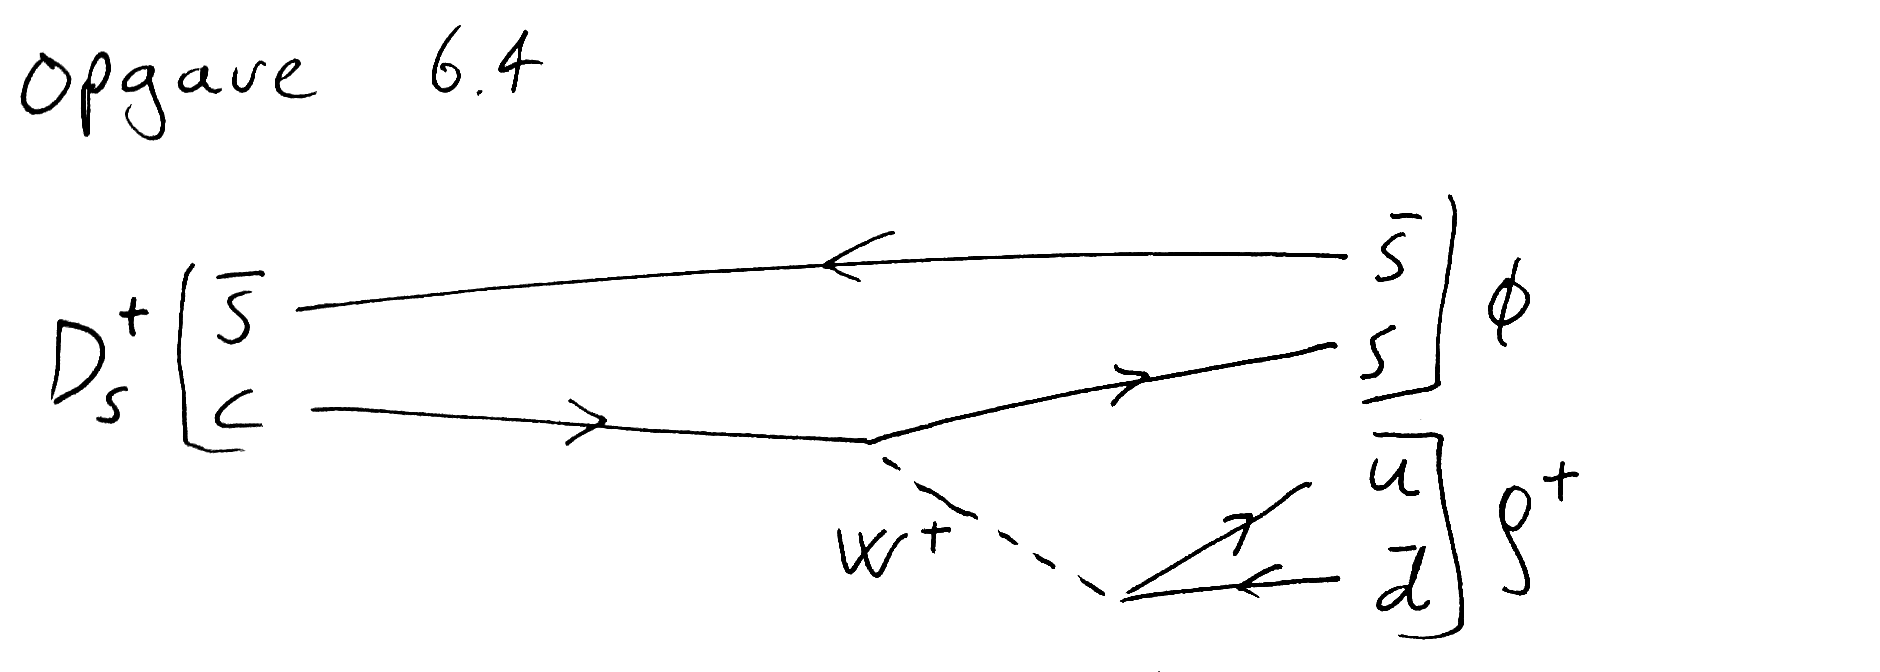
\includegraphics[width=0.4\textwidth]{KernePartikel/opg64.png}
  \caption{Feynmandiagram for henfald af $D^{+}_{s}$.}
  \label{fig:opg64}
\end{figure}
Se figur \ref{fig:opg64}.
\opg $\Omega^-(sss) \longrightarrow \Xi^-(dss) + \pi^0(u\bar{u})$
\begin{figure}[h]
  \centering
  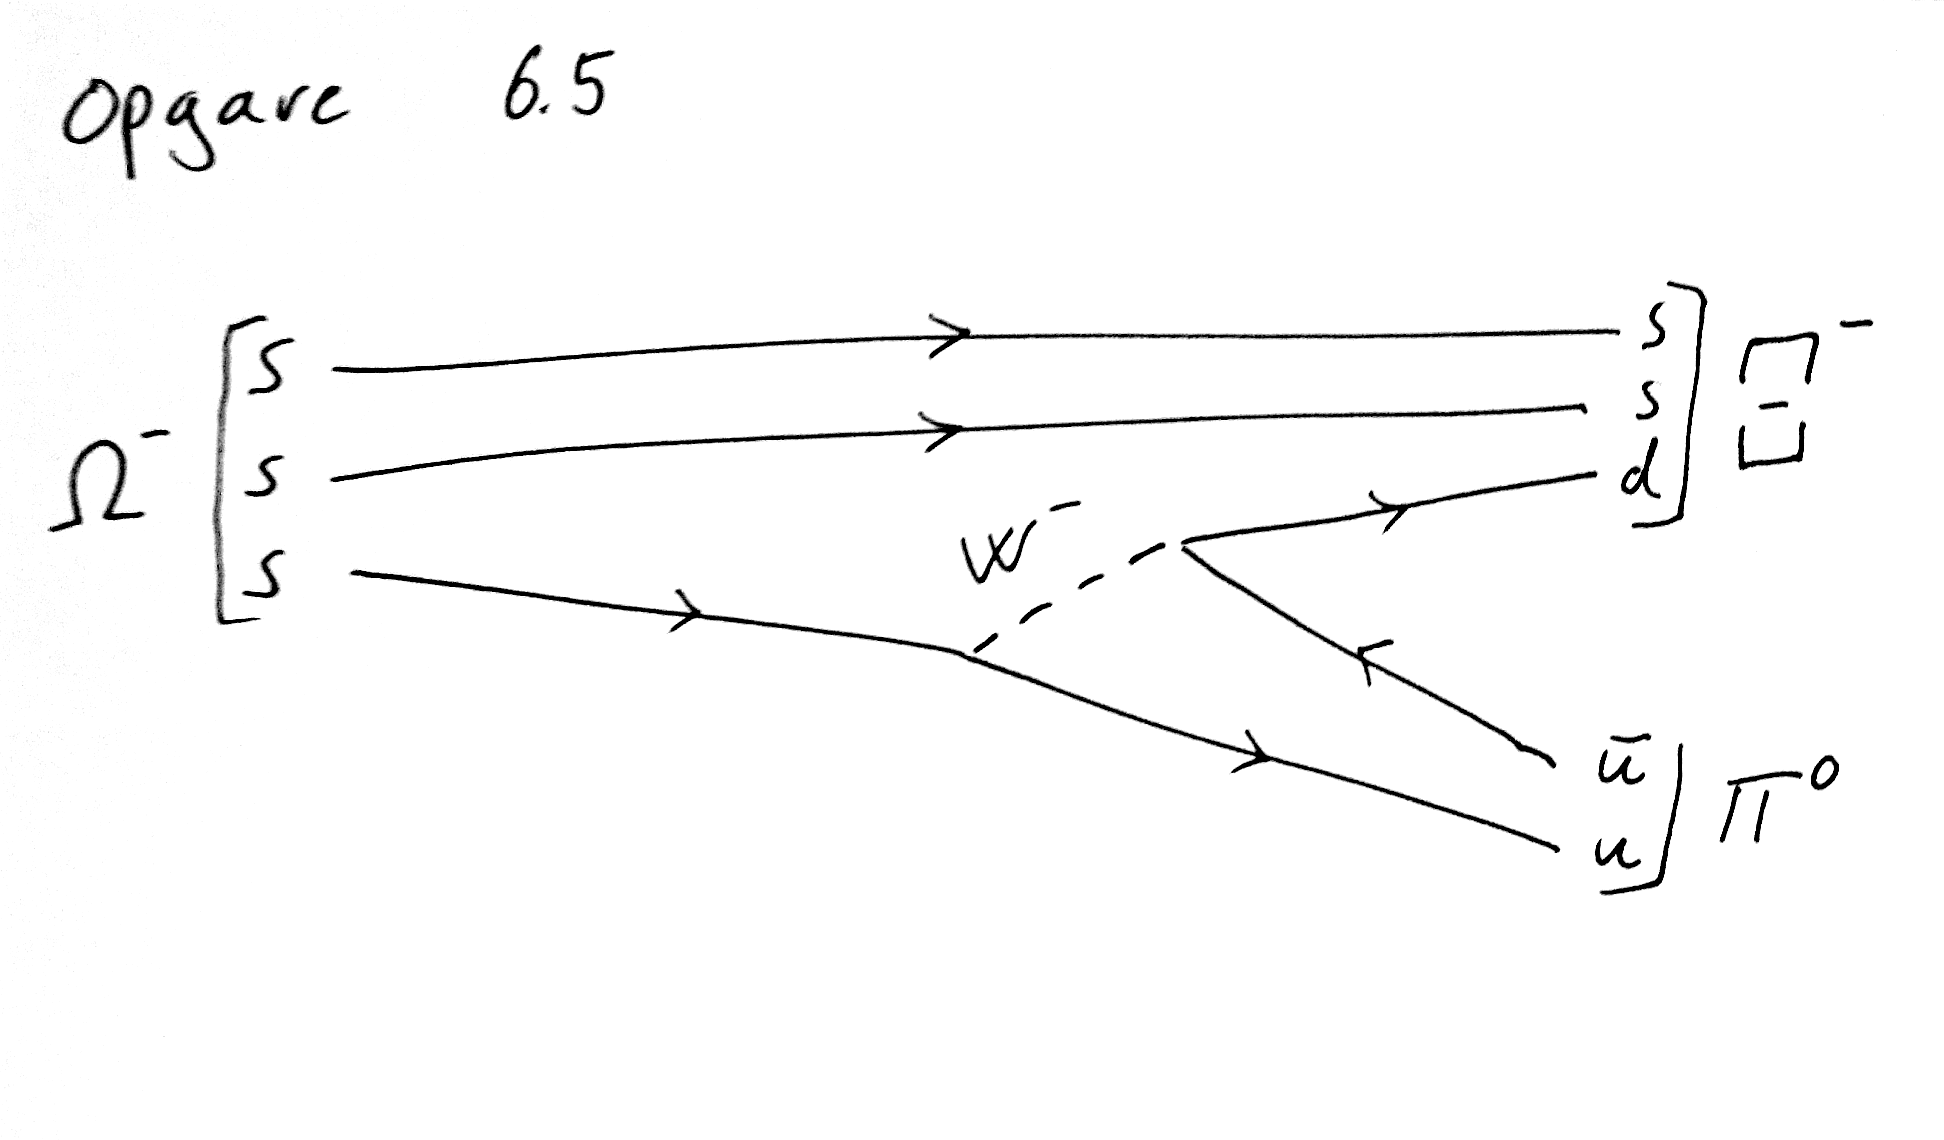
\includegraphics[width=0.4\textwidth]{KernePartikel/opg65.png}
  \caption{Feynmandiagram for henfald af $\Omega^-$.}
  \label{fig:opg65}
\end{figure}
Se figur \ref{fig:opg65}.
\end{opgave}
%%Når du starter på en opgave skriver du \begin{opgave}{navnet på opgaven}{sværhedsgrad}, hvor sværhedsgraden skrives som 1,2 eller 3, hvor 3 er den sværeste. 
%%Når opgaven er slut skrives \end{opgave}. 
%%Såfremt der er delopgaver skrives delopgaver som \opg 
%
%%Eksempel på opgave 
%%\begin{opgave}{Polære koordinater}{1}
%  %Den kinetiske energi af et legeme, der bevæger sig i 2D-planet er
%  %i kartesiske koordinater ($x$ og $y$) givet ved ligning
%  %(1.11).
%  %
%  %\opg Beregn $\dt{x}$ og $\dt{y}$ i polære koordinater og vis
%  %derefter, at den kinetiske energi udtrykt i polære koordinater er
%  %givet ved ligning (1.12).
%%\end{opgave}
\chapter{Elektromagnetiske Bølger Opgaver}
\section*{træningsmatematik}

\begin{opgave}{Gradient}{1}
Find gradienten ($\v \nabla f$) af følgende funktioner:
\opg$f(x,y) = x$
\opg$f(x,y) = x^2-y^2$
\opg$f(x,y) = xy+\cos(xy)$
\opg$f(x,y,z) = x^3+xy^2+xyz$
\opg$f(x,y,z) = \frac{\cos(x)+\sin(y)}{z}$
\end{opgave}

\begin{opgave}{Divergens}{1}
Find divergensen ($\v \nabla \cdot \v F$) af følgende funktioner:
\opg$\v F(x,y) = x^2\xhat+y^2\yhat$
\opg$\v F(x,y) = \xy{x^2y}{-xy^2}$
\opg$\v F(x,y,z) = \sin(x)\xhat+\cos(y)\yhat$
\opg$\v F(x,y,z) = x^2\xhat+y^2\yhat-\mathrm{e}^z$
\opg$\v F(x,y) = \xyz{x^2\cos(y)}{y^2\cos(z)}{z^2\cos(x)}$
\opg$\v F(x,y) = \mathrm{e}^z(y^2\xhat+x^2\yhat)$
\end{opgave}

\begin{opgave}{Rotation}{2}
Find rotationen ($\v \nabla \times \v F$) af følgende funktioner:
\opg$\v F(x,y,z) = x^2\xhat+y^2\yhat$
\opg$\v F(x,y,z) = \xyz{x^2y}{-xy^2}{0}$
\opg$\v F(x,y,z) = \sin(x)\xhat+\cos(y)\yhat$
\opg$\v F(x,y,z) = -y^2\xhat+x^2\yhat-\mathrm{e}^z$
\opg$\v F(x,y,z) = \xyz{x^2\cos(y)}{y^2\cos(z)}{z^2\cos(x)}$
\opg$\v F(x,y,z) = \mathrm{e}^z(y^2\xhat+x^2\yhat)$
\end{opgave}



\begin{opgave}{Bølgeligningen}{2}
Er de følgende funktioner løsninger til bølgeligningen: 
$$
\frac{\partial^3 f}{\partial z^3} = \frac{1}{v^2}\frac{\partial^2 f}{\partial t^2}
$$
\opg $f(z,t) = z^2+t^2$
\opg $g(z,t) = \cos(kz-\omega t)+\sin(2kz+2\omega t)$
\opg $h(z,t) = \cos(kz)\cos(\omega t)$
\opg $i(z,t) = \cos(zt)$
\end{opgave}

\begin{opgave}{Gange matrix med vektor}{1}
Givet matricen $\v A$ og en vektor $\v v$, hvad er $\v A\v v$ for forskellige $\v v$
$$
\v A = \begin{bmatrix}
1&2\\0&3
\end{bmatrix}
$$
\opg $\v v = \xy{1}{0}$
\opg $\v v = \xy{0}{1}$
\opg $\v v = \xy{1}{1}$
\opg $\v v = \xy{1}{-1}$
\opg $\v v = \xy{3}{4}$
\opg Er der noget særligt ved nogle af vektorerne?
\end{opgave}

\begin{opgave}{Matrix multiplikation}{1}
Udregn følgende matrix regnestykker.
\opg $\begin{bmatrix}
1&0\\0&-1
\end{bmatrix}
\begin{bmatrix}
-5&2\\4&3
\end{bmatrix}
$
\opg $\begin{bmatrix}
1&2\\0&3
\end{bmatrix}
\begin{bmatrix}
1&2\\0&3
\end{bmatrix}
$
\opg $\begin{bmatrix}
1&2\\0&3
\end{bmatrix}
\begin{bmatrix}
3&-2\\0&1
\end{bmatrix}
$
\opg $\begin{bmatrix}
0&-1\\1&0
\end{bmatrix}^4
$
\opg $\begin{bmatrix}
0&0\\1&0
\end{bmatrix}^2
$
\opg $\begin{bmatrix}
1&2\\0&3
\end{bmatrix}
\begin{bmatrix}
7&-4\\1&-5
\end{bmatrix}
$
\end{opgave}

\begin{opgave}{Genereliserede vektorer (Bonus)}{2}
Vi har indtil vidre brugt vektorer til at beskrive størrelser der har en retning og en længde. Dette er en vigtig egenskab ved vektorer, men matematisk er alt der lægges sammen og ganges med skalarer som vektorer også vektorer. Blandt andet gælder det for polynomier (og alle andre funktioner). Det er derfor muligt at oversætte polynomier til koordinatvektorer. Vi vil her se på andengradspolynomier oversat til 3-diminsionelle vektorer.
\begin{equation}
\xyz{1}{0}{0} \equiv p_2(x)=x^2~~~~~\xyz{0}{1}{0} \equiv p_1(x) = x ~~~~\xyz{0}{0}{1} \equiv  p_0(x)=1
\end{equation}
\opg Hvad bliver parabelen $f(x) = ax^2+bx+c$ som koordinatvektor.
\opg Differentier $p_2$, $p_1$ og $p_0$, og brug det til at opstille matricen $\v D$ der beskriver differentiering.
\opg Find dobbelt differentialet $D^2$ og tripelt differenitalet $D^3$ med matrix multiplikation. Stemmer det overens med hvad du ville forvente?
\\\\Spejer man grafen i $y$-aksen svarer det til at skifte fortegn på inputtet af funktionen: $f(x)$ bliver $f(-x)$. Dette kaldes også for paritet.
\opg Find den matrix $\v P$ der beskriver paritets transformationen af en parabel.
\opg Find $\v D\v P$ og $\v P \v D$. Har det en betydning om man tager paritet før man differentierer eller efter.
\\\\
\emph{Bemærk}: Man ganger 3-dimensionelle matricer sammen på samme måde som 2-dimensionelle.
\begin{align}
\begin{bmatrix}
a&b&c\\
d&e&f\\
g&h&i
\end{bmatrix}
\xyz{v_1}{v_2}{v_3} &= \xyz{av_1+bv_2+cv_3}{dv_1+ev_2+fv_3}{gv_1+hv_2+iv_3}\\
\begin{bmatrix}
a_1&b_1&c_1\\
d_1&e_1&f_1\\
g_1&h_1&i_1
\end{bmatrix}
\begin{bmatrix}
a_2&b_2&c_2\\
d_2&e_2&f_2\\
g_2&h_2&i_2
\end{bmatrix}
&=\begin{bmatrix}
a_1a_2+b_1d_2+c_1g_2&a_1b_2+b_1e_2+c_1h_2&a_1c_2+b_1f_2+c_1i_2\\
d_1a_2+e_1d_2+f_1g_2&d_1b_2+e_1e_2+f_1h_2&d_1c_2+e_1f_2+f_1i_2\\
g_1a_2+h_1d_2+i_1g_2&g_1b_2+h_1e_2+i_1h_2&g_1c_2+h_1f_2+i_1i_2
\end{bmatrix}
\end{align}
\end{opgave}

\begin{opgave}{En elektrisk ladet plade}{1}
\label{em:gauss}
En elektrisk ladet plade med tykkelse $l$ ligger i $xy$-planen. Det elektriske felt er $E_z=A$ ovenover pladen, $E_z=Bz$ inde i pladen og $E_z=C$ under pladen.
$$
E_z = 
\begin{cases}
A~~\text{for}~~z\geq \frac{l}{2}\\
Bz~~\text{for}~~\frac{l}{2}\geq z\geq \frac{-l}{2}\\
C~~\text{for}~~\frac{-l}{2}\geq z
\end{cases}
$$
\opg Hvis den elektriske feltstyrke skal være kontinuert, Hvad er $A$ og $C$ udtryk i $B$
\opg Brug Gauss lov til at finde ladningstætheden langs $z$-aksen i de tre intervaller.
\end{opgave}

\begin{opgave}{Tre dimmensionelle ladningsfordelinger}{2}
Brug Gauss lov til at finde ladningsfordelingerne der giver de følgende felter:
\opg $\v{E} =A\hat{\v z}$
\opg $\v{E} =\frac{A}{3}(\hat{\v x}+\hat{\v y}+\hat{\v z})$
\opg $\v{E} =Az^2\hat{\v z}$
\opg $\v{E} =Ay^3\hat{\v y}$
\opg $\v{E} =A(z^2\hat{\v z}+y^3\hat{\v y})$
\opg $\v{E} =\frac{A}{xy}(\hat{\v x}+\hat{\v y}+\hat{\v z})$
\end{opgave}

\begin{opgave}{Integralformen af Gauss lov}{3}
Vi ser på samme plade som i opgave \ref{em:gauss}.
Flux er et mål for hvor meget et f.eks. elektrisk felt der går igennem en overflade: $$\Phi_E = \iint \v{E}\cdot\mathrm{d}\v{a} = \iint E \cos \theta \mathrm{d}a$$ $\theta$ er vinkelen imellem feltet og overfladens normalvektor. Gauss lov kan også skrives med integraler:
\begin{equation}
\oiint \v{E}\cdot \mathrm{d}\v{a} = \frac{Q_\text{enc}}{\varepsilon_0}
\end{equation}
Det betyder at fluxen ud igennem en lukket (p.g.a. cirkelen i integraltegnet) overflade er proportional med ladningen inden for overfladen.
\opg Find fluxen igennem et kvadrat med sidelængde $s$ inde i pladen der er parallelt med den.
\opg Find Find fluxen igennem et kvadrat med sidelængde $s$ inde i pladen der er vinkelret på den.
\opg Find fluxen ud igennem en kube med sidelængde $s$, som summen af fluxen igennem kuben sider.
\opg Burg integral formen af Gauss lov til at finde den gennemsnitlige ladningstæthed i kuben.
\\\\
~~(Hint: Integralet af en konstant er konstanten gange det område der er blevet integreret over, for dobbelte integraler er det et areal.)
\end{opgave}

\begin{opgave}{Faradays lov}{2}
Et varierende magnetisk felt skaber et elektrisk felt $\v E =Ay\omega\cos (\omega t)\hat{\v z}$.
\opg Brug Faradays lov til at finde $\frac{\partial \v B}{\partial t}$.
\opg Hvad er $\v B$.
\\\\~~(Hint: $\int \cos(ax)\mathrm{d}x=\frac{\sin(ax)}{a}+k$)
\end{opgave}

\begin{opgave}{Frekvens og bølgelængde}{1}
Find frekvensen af den elektromagnetiske stråling for de forskellige bølgelængder:
\opg Mikrobølger: $\lambda = 12,2\text{ cm}$
\opg Rødt lys: $\lambda = 632\text{ nm}$
\opg Röntgenstråling: $\lambda = 1,54\text{ Å}=0,154\text{ nm}$
\opg $\gamma$-stråling: $\lambda = 1,87\text{ pm}$
\end{opgave}

\begin{opgave}{Lineært Polariseret Lys}{1}
Lav en skitse af en opstilling der består af en horisontal polarisator og vertikal polarisator. Vi sender nu upolariseret lys ind i opstillingen. 
\opg Ser du noget lys efter den horisontale polarisator? Hvorfor? Hvorfor ikke?
\opg Hvorfor ser du ikke noget lys efter den vertikale polarisator? 
\opg Hvilken lineær polarisator skal du så sætte ind for at kunne se lys efter den vertikale polarisator? Hvor skal den placeres? 
\end{opgave}

\begin{opgave}{Forskellige måder at regne med Jones Matricer}{1}
I denne opgave skal I se, hvordan man kan finde den resulterende Jones vektor for polariseret lys, der sendes igennem et lineært polariseringsfilter med horisontal TA efterfulgt af en rotator, på to forskellige måder. I skal også se, at rækkefølgen er vigtig, når man regner med Jones matricer.  
\opg Tag den generelle Jones vektor for polariseret lys og gang denne med Jones matricen for filteret. Tag herefter den resulterende vektor og gang denne med Jones matricen for en rotator.
\opg Tag de to Jones matricer fra 1), gang dem sammen (husk rigtig rækkefølge) og gang så den resulterende matrix på den generelle Jones vektor. Sammenlign resultatet med det du fik i 1). Stemmer det med hvad du forventede? Hvorfor? Hvorfor ikke?
\opg Gentag 2) men prøv denne gang at bytte rundt på rækkefølgen af Jones matricerne. Sammenlign med resultatet fra 1) og 2). Stemmer det med hvad du forventede? Hvorfor? Hvorfor ikke?    
\end{opgave}

\begin{opgave}{Lineære Polarisatorer}{3}
I denne opgave skal vi kigge på transmission af lineært polariseret lys efter det har rejst gennem lineære polarisatorer. 
Først introduceres intensiteten af lyset som afhænger af det elektriske felt, $E$. 
\begin{equation}
I = \frac{1}{2}\varepsilon_0c\v{E}\v{E^*}, 
\end{equation}
hvor $\v{E^*}$ er den \emph{kompleks konjugerede} matrix af $\v{E}$. Man kompleks konjugerer en matrix ved at transponere den og skifte fortegn i de komplekse indgange (indgange, der indeholder $i$). I tilfælde, hvor matricen ikke er kompleks, transponerer man blot matricen. 
Hvis $\v{E} = \xy{a}{b}$ (som ikke er kompleks!), er
\begin{equation}
\v{E^*}=\begin{bmatrix} a & b \\ \end{bmatrix}.
\end{equation}
Derudover er $\v{E}^*\v{E} = |\v E_t|^2$. 
Transmissionen er forholdet mellem hvor meget intensitet, der kommer ud og hvor meget, der kommer ind, altså 
\begin{equation}
T = \frac{I_{\text{t}}}{I_{\text{i}}} = \frac{\v{E_{\text{t}}}\v{E_{\text{t}}^*}}{\v{E_{\text{i}}}\v{E_{\text{i}}^*}},
\end{equation}
hvor subcript t er for \emph{transmitteret} intensitet/elektrisk felt og subscript i er for \emph{indkommende} intensitet/elektrisk felt. For lineært polariseret lys er det indkommende elektriske felt, som tidligere nævnt, givet ved 
\begin{equation}
\v{E_{\text{i}}}=\xy{\cos\alpha}{\sin\alpha},
\end{equation}
hvor $\alpha$ er vinklen i forhold til polariseringsaksen. 
\opg Linært polariseret lys rejser gennem en lineær polarisator med horisontal TA. Beregn transmissionen som funktion af $\alpha$, $T(\alpha)$. 
\opg Skitsér $T(\alpha)$. Hvad fortæller den?\\

Der bruges nu tre lineære polarisatorer. En med vertikal TA, en med horisontal TA og en med en 45$\degree$ TA. Det oplyses at $\cos(45\degree) = \sin(45\degree) = \frac{1}{\sqrt{2}}$. 
\opg Beregn Jones Matricen for den lineære polarisator med en 45$\degree$ TA.  
\opg Beregn $T(\alpha)$ når lineært polariset lys rejser gennem Horisontal polarisator $\rightarrow$ 45$\degree$ polarisator $\rightarrow$ vertikal polarisator. 
\end{opgave}

\begin{opgave}{Faseforskydere}{3}
Et andet optisk element er en såkaldt \emph{faseforskyder}. Halvbølge plader og kvartbølge plader er eksempler på faseforskydere. Som navnet antyder påvirker en faseforskyder fasen i det elektriske felt. 

Det elektriske felt $E = E_0\cos(kz-\omega t)$ starter i (0,0), men det kan ændres ved at tilføje en fase, $\phi$. Fasen forskyder således startpunktet for bølgen, som det elektriske felt kan beskrives ved. Med fasen er $E = E_0\cos(kz-\omega t + \phi)$. Afstanden mellem to toppe i en cosinus funktion svarer til $2\pi$ i radianer, og man angiver derfor altid fasen som et tal gange $\pi$. Det elektrisk felt er her skrevet på sin reelle form, men i mange fysiske sammenhænge er det nemmere at skrive feltet på sin komplekse form. Den komplekse funktion $e^{iA} = \cos(A) + i\sin(A)$, hvor det første led er den real--delen og det sidste led er imaginær--delen. 
I arbejde med elektriske felter er blot et redskab, så den imaginære del af det elektriske felt har ingen fysisk betydning. Feltets komplekse form er givet ved 
\begin{equation}
E = E_0e^{i(kz - \omega t + \phi)}, 
\end{equation}
og da det elektriske felt består af en $x$-- og $y$--komponent er 
\begin{equation}
\v{E} = E_{0x}e^{i(kz - \omega t + \phi_x)}\hatvec{x} + E_{0y}e^{i(kz - \omega t + \phi_y)}\hatvec{y} = \left[E_{0x}e^{i\phi_x}\hatvec{x} + E_{0y}e^{i\phi_y}\hatvec{y}\right]e^{i(kz-\omega t)}. 
\end{equation}
En faseforskyder transformerer så
\begin{equation}
E_{0x}e^{i\phi_x} \,\,\,\,\, \text{til} \,\,\,\,\, E_{0x}e^{i(\phi_x + \varepsilon_x)}
\end{equation}
og 
\begin{equation}
E_{0y}e^{i\phi_y} \,\,\,\,\, \text{til} \,\,\,\,\, E_{0y}e^{i(\phi_y + \varepsilon_y)},
\end{equation}
hvor $\varepsilon_x$ og $\varepsilon_y$ kaldes for \emph{slow axis} og \emph{fast axis}, og de er altså en ekstra fase. 
Jones Matricen for en faseforskyder er derfor 
\begin{equation}
\v{M} = \begin{bmatrix}
e^{i\varepsilon_x} & 0 \\
0 & e^{i\varepsilon_y} \\
\end{bmatrix}.
\end{equation}
En faseforskyder kan f.eks. være enten en halvbølge plade eller kvartbølge plade. Differencen mellem $\varepsilon_x$ og $\varepsilon_y$ er det, der afgør, om det er den ene eller anden. Hvis $|\varepsilon_x-\varepsilon_y| = \pi$ er den en halvbølgeplade, mens den er en kvartbølge plade når $|\varepsilon_x-\varepsilon_y| = \frac{\pi}{2}$. 

Vi skal nu se på en opstilling, der i rækkefølge består af en kvartbølgeplade og en lineær polaristor med vertikal TA. Lyset er til at starte med horisontalt lineært polariseret. 

Vi ønsker at kunne rotere kvartbølge pladen med en vinkel $\theta$ og dermed bestemme transmissionen af lyset som funktion af denne vinkel. Jones Matricen for kvartbølgepladen $M$ er derfor ikke nok, da den ikke tager højde for, at kvartbølgepladen og skal rotere. Jones Matricen for en roterende kvartbølge plade er derfor 
\begin{equation}
\tilde{\v{M}} = \v{R} \v{M} \v{R}^{-1}, 
\end{equation}
hvor $\v{R}$ er rotator matricen og 
\begin{equation}
\v{R}^{-1} = \begin{bmatrix}
\cos\theta & \sin\theta \\
-\sin\theta & \cos\theta \\
\end{bmatrix}.
\end{equation}
\opg Beregn $\tilde{\v{M}}$ for en kvartbølgeplade. 
\opg Beregn $T_v(\theta)$ for når lyset er rejst gennem opstillingen. \emph{Hint: $i^2=-1$}. Skitsér $T_v(\theta)$. 
\opg Beregn $T_h(\theta)$ for samme opstilling, men hvor den vertikale lineær polarisator nu er skiftet ud med en horisontal lineær polarisator. Skitser $T_h(\theta)$
\opg Beregn $\tilde{\v{M}}$ for en halvbølge plade og gentag beregning er $T_{v/h}(\theta)$ for opstillingen når den indeholder en vertikal lineære polarisator og når den indeholder en horisontal lineær polarisator. Skitsér $T_v(\theta)$ og $T_h(\theta)$. 
\end{opgave}

\newpage
\chapter{Elektromagnetiske bølger Facitliste}
\begin{opgave}{Gradient}{1}
\opg $f(x,y) = x ~~~~\v\nabla f(x,y) = \xhat = \xy{1}{0}$
\opg $f(x,y) = x^2-y^2 ~~~~\v\nabla f(x,y) = x\xhat-y\yhat=\xy{x}{y}$
\opg $f(x,y) = xy+\cos(xy) ~~~~\v\nabla f(x,y) = (y-x\sin(xy))\xhat+(x-y\sin(xy))\yhat = \xy{y-x\sin(xy)}{x-y\sin(xy}$
\opg $f(x,y,z) = x^3+xy^2+xyz ~~~~\v\nabla f(x,y) = (3x^2+y^2+yx)\xhat+(2xy+xz)\yhat+xy\zhat = \xyz{3x^2+y^2+yz}{2xy+xz}{xy}$
\opg $f(x,y,z) = x ~~~~\v\nabla f(x,y) = \frac{-\sin(x)}{z}\xhat+\frac{\cos(y)}{z}\yhat-\frac{1}{z^2}\zhat = \frac{1}{z}\xyz{-\cos(x)}{\sin(y)}{-1/z}$
\end{opgave}


\begin{opgave}{Divergens}{1}
Find divergensen ($\v \nabla \cdot \v F$) af følgende funktioner:
\opg$\v F(x,y) = x^2\xhat+y^2\yhat~~~~\v\nabla\cdot F = 2x+2y$
\opg$\v F(x,y) = \xy{x^2y}{-xy^2}~~~~\v\nabla\cdot F = 2xy-2xy= 0$
\opg$\v F(x,y,z) = \sin(x)\xhat+\cos(y)\yhat~~~~\v\nabla \cdot F = \cos(x)-\sin(y)$
\opg$\v F(x,y,z) = x^2\xhat+y^2\yhat-\mathrm{e}^z~~~~\v\nabla\cdot F = 2x+2y+\mathrm{e}^z$
\opg$\v F(x,y) = \xyz{x^2\cos(y)}{y^2\cos(z)}{z^2\cos(x)}~~~~\v\nabla\cdot F = 2x\cos(y)+2y\cos(z)+2z\cos(x)$
\opg$\v F(x,y) = \mathrm{e}^z(y^2\xhat+x^2\yhat)~~~~\v\nabla\cdot F = 0$
\end{opgave}

\begin{opgave}{Rotation}{2}
Find rotationen ($\v \nabla \times \v F$) af følgende funktioner:
\opg$\v F(x,y,z) = x^2\xhat+y^2\yhat ~~~~\v\nabla \times F = \v 0$
\opg$\v F(x,y,z) = \xyz{x^2y}{-xy^2}{0} ~~~~\v\nabla \times F =\xyz{0}{0}{-x^2-y^2}$
\opg$\v F(x,y,z) = \sin(x)\xhat+\cos(y)\yhat ~~~~\v\nabla \times F =\v 0$
\opg$\v F(x,y,z) = -y^2\xhat+x^2\yhat-\mathrm{e}^z ~~~~\v\nabla \times F =2x+2y$
\opg$\v F(x,y,z) = \xyz{x^2\cos(y)}{y^2\cos(z)}{z^2\cos(x)} ~~~~\v\nabla \times F =xyz{y^2\sin(z)}{-z^2\sin(x)}{-x^2\sin(y)}$
\opg$\v F(x,y,z) = \mathrm{e}^z(y^2\xhat+x^2\yhat) ~~~~\v\nabla \times F =\xyz{-\mathrm{e}^zx^2}{-\mathrm{e}^zy^2}{2\mathrm{e}^z(x-y)}$
\end{opgave}


\begin{opgave}{Bølgeligningen}{2}
Er de følgende funktioner løsninger til bølgeligningen: 
$$
\frac{\partial^2f}{\partial z^2} = \frac{1}{v^2}\frac{\partial^2 f}{\partial t^2}
$$
Man differentierer funktionen dobbelt til både $t$ og $z$. Er der kun en faktor til forskel er det en løsning.
\opg 
\begin{align*}
f(z,t) &= z^3+t^3\\
\frac{\partial f}{\partial z} &= 3z^2\\
\frac{\partial^2 f}{\partial z^2} &== 6z\\
\frac{\partial f}{\partial t} = 3t\\
\frac{\partial^2 f}{\partial t^2} = 6t
\end{align*}
Det er ikke en løsning.
\opg Her bruges kædereglen til differentiere funktionerne.
\begin{align*}
g(z,t) &=\cos(kz-\omega t)+\sin(2kz+2\omega t)\\
\frac{\partial g}{\partial z} &= -k\cos(kz-\omega t)+2k\cos(2kz-2\omega t)\\
\frac{\partial^2 g}{\partial t^2} &=-k^2\sin(kz-\omega t)-4k^2\sin(2kz-2\omega t)\\
\frac{\partial g}{\partial t} &= \omega\sin(kz-\omega t) -2\omega \cos(2kz-2\omega t)\\
\frac{\partial^2 g}{\partial t^2} &= -\omega^2\cos(kz-\omega t) - 4\omega^2\cos(2kz-2\omega t)\\
-k^2\frac{\partial^2 g}{\partial z^2} &= -\omega^2 \frac{\partial^2 g}{\partial t^2}~~\text{Gælder, så det er en løsning.}\\
v&=\frac{\omega}{k}~~\text{~Er bølgens hastighed.} 
\end{align*}
Bølgeligningen hører til en kategori af velopdragne differentialligninger hvor summen af to løsninger også er en løsning. De kaldes lineære differentialligninger.
\opg
\begin{align*}
h(z,t) &= \cos(kz)\cos(\omega t)\\
\frac{\partial h}{\partial z} &= -k\sin(kz)\cos(\omega t)\\
\frac{\partial^2 h}{\partial z^2} &= -k^2\cos(kz)\cos(\omega t)\\
\frac{\partial h}{\partial t} &= -\omega \cos(kz)\sin(\omega t)\\
\frac{\partial^2 h}{\partial t^2} &= -\omega^2 \cos(kz)\cos(\omega t)\\
-k^2\frac{\partial^2 h}{\partial z^2} &= -\omega^2\frac{\partial^2 h}{\partial t^2}~~\text{Det er en løsning}\\
v &= \frac{\omega}{k}~~\text{er hastigheden af bølgen}
\end{align*}
Dette er iøvrigt en stående bølge. Den kan også meskrives som to bølger med den halve amplitude og rejsende i hver sin retning.
\opg
\begin{align*}
i(z,t) &= \cos(zt)\\
\frac{\partial i}{\partial z} &= -t\sin(zt)\\
\frac{\partial^2 i}{\partial^2 z} &= -t^2\cos(zt)\\
\frac{\partial i}{\partial t} &= -z\sin(zt)\\
\frac{\partial^2 i}{\partial t^2} &= -z^2\cos(zt)
\end{align*}
Det er ikke en løsning.
\end{opgave}

\begin{opgave}{Gange matrix med vektor}{1}
Givet matricen $\v A$ og en vektor $\v v$, hvad er $\v A\v v$ for forskellige $\v v$
$$
\v A = \begin{bmatrix}
1&2\\0&3
\end{bmatrix}
$$
\opg $\v v = \xy{1}{0}~~~~\v A\v v  = \xy{1}{0}$
\opg $\v v = \xy{0}{1}~~~~\v A\v v  = \xy{2}{3}$
\opg $\v v = \xy{1}{1}~~~~\v A\v v  = \xy{3}{3}$
\opg $\v v = \xy{1}{-1}~~~~\v A\v v  = \xy{-1}{-3}$
\opg $\v v = \xy{3}{4}~~~~\v A\v v  = \xy{11}{12}$
\opg Er der noget særligt ved nogle af vektorerne? $\xy{1}{0}$ og $\xy{1}{1}$ er egenvektorer for $\v A$. De giver sigselv gange en faktor.
\end{opgave}


\begin{opgave}{Matrix multiplikation}{1}
Udregn følgende matrix regnestykker.
\opg $\begin{bmatrix}
1&0\\0&-1
\end{bmatrix}
\begin{bmatrix}
-5&2\\4&3
\end{bmatrix} = \begin{bmatrix}
-5&2\\-4&-3
\end{bmatrix}
$
\opg $\begin{bmatrix}
1&2\\0&3
\end{bmatrix}
\begin{bmatrix}
1&2\\0&3
\end{bmatrix}=
\begin{bmatrix}
1&8\\0&9
\end{bmatrix}
$
\opg $\begin{bmatrix}
1&2\\0&3
\end{bmatrix}
\begin{bmatrix}
3&-2\\0&1
\end{bmatrix}=
\begin{bmatrix}
3&0\\0&3
\end{bmatrix}
$
\opg $\begin{bmatrix}
0&-1\\1&0
\end{bmatrix}^4=\begin{bmatrix}
1&0\\0&1
\end{bmatrix}
$
\opg $\begin{bmatrix}
0&0\\1&0
\end{bmatrix}^2
=
\begin{bmatrix}
0&0\\0&0
\end{bmatrix}
$
\opg $\begin{bmatrix}
1&2\\0&3
\end{bmatrix}
\begin{bmatrix}
7&-4\\1&-5
\end{bmatrix}
=
\begin{bmatrix}
9&-14\\
3&15
\end{bmatrix}
$
\end{opgave}

\begin{opgave}{Genereliserede vektorer}{2}
\opg $f(x) = ax^2+bx+c$ bliver $ap_2(x)+bp_1(x)+cp_0(x) = \xyz{a}{b}{c}$.
\opg $\frac{d}{dx}p_2(x) = 2x = 2p_1(x)$\\
$\frac{d}{dx}p_1(x) = 1 = p_0(x)$\\
$\frac{d}{dx}p_0(x) = 0$\\
De differentierede koordinatvektorer sættes ind som søjler i matricen.\\
$\v D = \begin{bmatrix}
0&0&0\\
2&0&0\\
0&1&0
\end{bmatrix}
$
\opg $\v D^2 = \begin{bmatrix}
0&0&0\\
0&0&0\\
2&0&0
\end{bmatrix}$\\
$\v D^3 = \begin{bmatrix}
0&0&0\\
0&0&0\\
0&0&0
\end{bmatrix}$
\opg
Samme fremgangsmåde som opgave 1\\
$p_2(-x) = (-x)^2 = x^2=p_2(x)$\\
$p_1(-x) = -x = -p_1(x)$\\
$p_0(-x) = 1 =p_1(x)$\\
$\v P = \begin{bmatrix}
1&0&0\\
0&-1&0\\
0&0&1
\end{bmatrix}$
\opg
$\v D \v P=\begin{bmatrix}
0&0&0\\
2&0&0\\
0&-1&0
\end{bmatrix}$\\
$\v P\v D = \begin{bmatrix}
0&0&0\\
-2&0&0\\
0&1&0
\end{bmatrix}$
\end{opgave}

\begin{opgave}{En elektrisk ladet plade}{1}
\opg Hvis feltet skal være kontinuert vil $E_z\left(\frac{l}{2}\right)=A=B\frac{l}{2}$ på oversiden og tilsvarende: $E_z\left(\frac{-l}{2}\right)=-B\frac{l}{2}=C$.
\opg $\rho = \v \nabla \v E \varepsilon_0 = \frac{\partial E_z}{\partial z}\varepsilon_0$. På begge sider af pladen er det nul. inde i pladen er det: $\rho = B\varepsilon_0$
\end{opgave}

\begin{opgave}{Tre dimmensionelle ladningsfordelinger}{2}
Brug Gauss lov til at finde ladningsfordelingerne der giver de følgende felter:
\opg $\v{E} =A\hat{\v z} = 0$
\opg $\v{E} =\frac{A}{3}(\hat{\v x}+\hat{\v y}+\hat{\v z}) = 0$
\opg $\v{E} =Az^2\zhat = 2Az$
\opg $\v{E} =Ay^3\yhat = 3Ay^2$
\opg $\v{E} =A(z^2\hat{\v z}+y^3\hat{\v y}) = A(2z+3y)$
\opg $\v{E} =\frac{A}{xy}(\hat{\v x}+\hat{\v y}+\hat{\v z}) = -A\left(\frac{1}{x^2y}+\frac{1}{xy^2}\right)$
\end{opgave}

\begin{opgave}{Integralformen af Gauss lov}{3}
\opg
Siden kvadratet er parallelt med pladen ligge hele kvadratet i samme $z$. $\v E$-feltet er vinkelret på pladen så, med hjælp fra hintet er fluxen:
$$
\Phi_E(z) = \iint E_z \mathrm{d}a = E_zs^2 = Bzs^2
$$
\opg
Er kvadratet vinkelret på pladen vil $\cos\theta=0$ derfor er fluxen det også.
\opg
Husk at man måler fluxen ud af kuben. Toppen og bunden af kuben er parallelle med pladen, så de bidrager med $Bzs^2$ resten af siderne er vinkelrette så de bidrager ikke.
Placeres kuben med centrum i en højde $z_0$ bliver den fluxen ud igennem den:
$$
\Phi_E = \Phi_E(z_0+\tfrac{l}{2})-\Phi_E(z_0-\tfrac{l}{2})=Bs^3
$$
Ud fra integralformen af Gauss lov findes den indesluttede ladning.
$$
Q_\text{encl} = Bs^3\varepsilon_0
$$
Derefter findes ladningstætheden ved at dele med rumfanget af kuben
$$
\rho_\text{gns} = \frac{Q_\text{encl}}{s^3} = B\varepsilon_0
$$
Dette virker kun fordi ladningstætheden er konstant, men gøres $s$ mindre vil man opnå et gradvist bedre resultat.
\end{opgave}

\begin{opgave}{Faradays lov}{2}
\opg Man tager rotationenaf $\v E$-feltet og bruger Faradays lov til at finde $\frac{\partial \v B}{\partial t}$.
$$
\frac{\partial \v B}{\partial t} = -\v \nabla \times \v E = -A\omega\cos(\omega t)\xhat
$$
\opg
Siden integration er det modsatte af diffentiation indsættes det i det givne integral.
$$
\v B = \int \frac{\partial \v B}{\partial t}\mathrm{d}t = -A\omega\xhat\int\cos(\omega t)\mathrm{d}t = -A\xhat\sin(\omega t)
$$
Der kan egentligt også være en konstant del af $\v E$-feltet, men vi kan ikke vide noget om den og antager derfor at den er nul.
\end{opgave}

\begin{opgave}{Frekven og bølgelængde}{1}
Brug sammenhængen $c = \nu\lambda\iff\nu=\frac{c}{\lambda}$.
\opg Mikrobølger: $\lambda = 12,2\text{ cm}~~~~~\nu = 2,46 \mathrm{GHz} = 2,46\cdot 10^9\mathrm{Hz}$
\opg Rødt lys: $\lambda = 632\text{ nm}~~~~~\nu = 474 \mathrm{THz} = 4,74\cdot 10^{12}\mathrm{Hz}$
\opg Röntgenstråling: $\lambda = 1,54\text{ Å}=0,154\text{ nm}~~~~~\nu = 1,95 \mathrm{EHz} = 2,46\cdot 10^{18}\mathrm{Hz}$
\opg $\gamma$-stråling: $\lambda = 1,87\text{ pm}~~~~~\nu = 160 \mathrm{EHz} = 2,46\cdot 10^{20}\mathrm{Hz}$
\end{opgave}

\begin{opgave}{Lineært Polariseret Lys}{1}
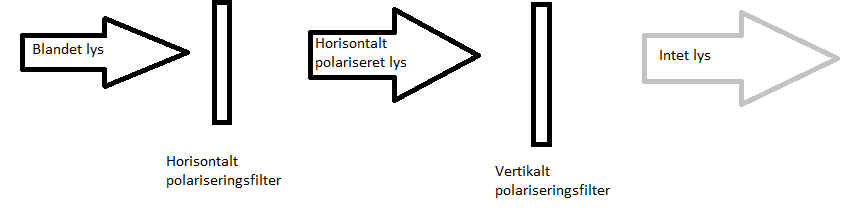
\includegraphics[width = \textwidth]{elektrodynamik/polskitse.png}
\opg Siden upolariseret lys består af en blanding af alle polariseringer vil noget af det komme igennem polariseringsfilteret.
\opg Efter det horisontale polariseringsfilter er lyset horisontalt polariseret, derfor kan intet komme igennem det vertikale polariseringsfilter.
\opg Indsættes et diagonalt polariseringsfilter imellem de to oprindelige filtre, vil det diagonale filter tillade noget af det horisontalt polariserede lys at passere, men bagefter er det være diagonalt polariseret, så noget af det kommer også igennem.
\end{opgave}

\begin{opgave}{Forskellige måder at regne med Jones Matricer}{1}
Generelt polariseret lys har Jones vektoren: $\v v = \xy{\cos \alpha}{\sin \alpha}$. Polariseringsfilteret har Jones matricen: 
$\v P = \begin{bmatrix}
1&0\\0&0
\end{bmatrix}$.
Rotatoren har Jones matricen: $\v R = \begin{bmatrix}
\cos\beta & -\sin\beta\\\sin\beta&\cos\beta
\end{bmatrix}$
\opg Filteret gange vektoren er:
$$
\begin{bmatrix}
1&0\\0&0
\end{bmatrix}
\xy{\cos\alpha}{\sin\alpha} = \xy{cos\alpha}{0}
$$
Denne vektor gange rotatoren bliver:
$$
\begin{bmatrix}
\cos \beta&-\sin\beta\\\sin \beta&\cos\beta
\end{bmatrix}
\xy{\cos\alpha}{0}=
\xy{\cos\alpha\cos\beta}{\cos\alpha\sin\beta}
$$
Hvis man vil kan man bruge trigonometriske identiteter til at omskrive det, men det bliver ikke pænere af det.
$$
\xy{\cos\alpha\cos\beta}{\cos\alpha\sin\beta}=
\frac{1}{2}\xy{\cos(\alpha-\beta)+\cos(\alpha+\beta)}{\sin(\alpha+\beta)-\sin(\alpha-\beta)}
$$
\opg Ganger man matricerne sammen får man:
$$
\v R\v P=
\begin{bmatrix}
\cos\beta&\sin\beta\\0&0
\end{bmatrix}
$$
Ganges denne matrix på vektoren fåes
$$
\begin{bmatrix}
\cos\beta & \sin\beta \\ 0 & 0
\end{bmatrix}
\xy{\cos\alpha}{\sin\alpha}=
\xy{\cos\alpha\cos\beta}{\cos\alpha\sin\beta}
$$
Rækkefølgen har ingen betydning. Dette gælder generelt for matricer og vektorer. Det kaldes den distributive lov.$\v A\v B\v C=(\v A\v B)\v C=\v A(\v B\v C)$
\opg
I den anden rækkefølge bliver det:
$$
\v P(\v R \v v ) = 
\begin{bmatrix}
1&0\\0&0
\end{bmatrix}
\begin{bmatrix}
\cos\beta & -\sin\beta\\\sin\beta&\cos\beta
\end{bmatrix}
\xy{\cos\alpha}{\sin\alpha}
=
\begin{bmatrix}
1&0\\0&0
\end{bmatrix}
\xy{\cos\alpha\cos\beta-\sin\alpha\sin\beta}{\cos\alpha\sin\beta+\sin\alpha\cos\beta}=
\xy{\cos\alpha\cos\beta-\sin\alpha\sin\beta}{0}
$$
Ganges matricerne samme først bliver det.
$$
\v P(\v R \v v ) = 
\begin{bmatrix}
1&0\\0&0
\end{bmatrix}
\begin{bmatrix}
\cos\beta & -\sin\beta\\\sin\beta&\cos\beta
\end{bmatrix}
\xy{\cos\alpha}{\sin\alpha}=
\begin{bmatrix}
\cos\beta&-\sin\beta\\
0&0
\end{bmatrix}
\xy{\cos\alpha}{\sin\beta}
=
\xy{\cos\alpha\cos\beta-\sin\alpha\sin\beta}{0}
$$
Bemærk at rækkefølgen af matricerne har betydning.
\end{opgave}

\begin{opgave}{Lineære Polarisatorer}{3}
\opg Den horisontale polarisator har Jones matricen $\v H=\begin{bmatrix}
1&0\\0&0
\end{bmatrix}$
Det transmiterede lys har Jones vektoren:
$$
\v E_t = \v H \v E_i = \begin{bmatrix}
1&0\\0&0
\end{bmatrix}
\xy{\cos\alpha}{\sin\alpha}
=
\xy{\cos\alpha}{0}
$$
Nu kan intensiteterne findes ud fra Jones vektorerne. Til $I_i$ anvendes Pythagoras sætning for en trekant i enhedscirkelen.
$$
|\v E_i|^2=\cos^2\alpha+\sin^2\alpha=1
$$
$$
|\v E_t|^2=\cos^2\alpha
$$
Transmitansen er dermed:
$$
T(\alpha)=\frac{|\v E_t|^2}{|\v E_i|^2}=\cos^2\alpha
$$
\opg Den blå graf på figuren er $T(\alpha)$
\opg Den generelle form for et lineært polariseringsfilter findes i kompendiet ligning (6.28). Den er:
$$
\v P(\theta)=\begin{bmatrix}
\cos^2\theta&\cos\theta\sin\theta\\
\cos\theta\sin\theta&\sin^2\theta
\end{bmatrix}
$$
Indsættes $\theta=45^\circ$ bliver alle indgangene $\frac{1}{2}$.
$$
\v P(45^\circ) = \begin{bmatrix}\tfrac{1}{2}&\tfrac{1}{2}\\\tfrac{1}{2}&\tfrac{1}{2}\end{bmatrix} = \frac{1}{2} \begin{bmatrix}
1 & 1 \\
1 & 1 \\
\end{bmatrix}
$$
%\opg
%Jones vektoren for lineært polariseret lys sendt igennem et diagonalt filter er:
%$$
%\v D\v E_i = \begin{bmatrix}
%\tfrac{1}{2}&\tfrac{1}{2}\\\tfrac{1}{2}&\tfrac{1}{2}
%\end{bmatrix}
%\xy{\cos\alpha}{\sin\alpha}
%=
%\frac{1}{2}\xy{\cos\alpha+\sin\alpha}{\cos\alpha+\sin\alpha}
%$$
%$|\v E_i|^2$ er uændret og lig 1, så $T=|\v E_t|^2$.
%$$
%T(\alpha)=\frac{1}{4}((\cos\alpha+\sin\alpha)^2+(\cos\alpha+\sin\alpha)^2)=\frac{1}{2}(\cos^2\alpha+\sin^2\alpha+2\cos\alpha\sin\alpha)
%=
%\frac{1}{2}+\cos\alpha\sin\alpha
%$$
%Denne funktion er plottet i rødt på figuren. Som man kan se er den forskudt $45^\circ$ i forhold til et horisontalt polariseringsfilter.
%Det er helt fint at slutte er, men det er muligt at gøre resultatr pænere med et par trigonometriske identiteter.
%$
%\cos u\sin v = \frac{1}{2}(\sin(u+v)-\sin(u-v))
%$
%Så bliver transmitansen:
%$$
%T(\alpha) = \frac{1}{2}+\frac{1}{2}(\sin(2\alpha)-\sin(0))=\frac{1}{2}(1+\sin(2\alpha))
%$$
%Herefter bruges:
%$
%\cos(u-90^\circ) = \sin u
%$
%
%$$
%T(\alpha) = \frac{1}{2}(1+\cos(2\alpha-90^\circ))=\frac{1}{2}(1+\cos(2(\alpha-45^\circ)))
%$$
%Den sidste identitet der bruges er: $\cos^2u=\frac{1}{2}(1+\cos(2u))$
%$$
%T(\alpha) = \cos^2(\alpha-45^\circ)
%$$
\includegraphics[scale=1]{elektrodynamik/Emskitse.eps}
\opg
Der er to måder at løse denne opgave på. Man kan enten gange de relevante Jones matricer på vektoren en af gangen, eller man kan gange matricerne sammen og derefter gange med vektoren. Her demonstreres kun den anden metode.
De relvante matricer er:
$$
\v H = \begin{bmatrix}
1&0\\0&0
\end{bmatrix}
~~~~~\v D=
\frac{1}{2}\begin{bmatrix}
1&1\\1&1
\end{bmatrix}
~~~~\v V = \begin{bmatrix}
0&0\\0&1
\end{bmatrix}
$$
Bemærk rækkefølgen af matricerne, da lyset først passerer den horisontale polarisator er den tilsvarende. Den endelige Jones matrix er dermed:
$$
\v M = \v{VDH}=
\frac{1}{2}
\begin{bmatrix}
0&0\\0&1
\end{bmatrix}
\begin{bmatrix}
1&1\\1&1
\end{bmatrix}
\begin{bmatrix}
1&0\\0&0
\end{bmatrix}
=
\frac{1}{2}
\begin{bmatrix}
0&0\\0&1
\end{bmatrix}
\begin{bmatrix}
1&0\\1&0
\end{bmatrix}
=
\frac{1}{2}
\begin{bmatrix}
0&0\\1&0
\end{bmatrix}
$$
Nu kan $\v E_t$ findes
$$
\v E_t = \v M \v E_i = \frac{1}{2}\begin{bmatrix}
0&0\\0&1
\end{bmatrix}
\xy{\cos\alpha}{\sin\alpha}
=
\frac{1}{2}\xy{0}{\cos\alpha}
$$
Så kan $T(\alpha)$ findes
$$
T(\alpha) = \frac{|\v E_t|^2}{|\v E_i|^2}=\frac{1}{4}\cos^2\alpha
$$
%Hvilket iøvrigt kan omskrives til:
%$$
%\frac{\cos^2(\alpha-90^\circ)}{4}
%$$
Intensiteten mindskes med en faktor 4 og det resulterende lys er vandret polariseret.
\end{opgave}

\begin{opgave}{Faseforskydere}{3}
\opg $\tilde{\v M}$ bliver
\begin{equation*}
\tilde{\v{M}} = 
\begin{bmatrix}
\cos\theta & -\sin\theta \\
\sin\theta & \cos\theta \\
\end{bmatrix}
\begin{bmatrix}
e^{i\varepsilon_x} & 0 \\
0 & e^{i\varepsilon_y} \\
\end{bmatrix}
\begin{bmatrix}
\cos\theta & \sin\theta \\
-\sin\theta & \cos\theta \\
\end{bmatrix}
=
\begin{bmatrix}
e^{i\varepsilon_x} \cos^2 \theta + e^{i\varepsilon_y} \sin^2 \theta & \left( e^{i\varepsilon_x}-e^{i\varepsilon_y} \right)\cos\theta\sin\theta \\
\left( e^{i\varepsilon_x}-e^{i\varepsilon_y} \right)\cos\theta\sin\theta & e^{i\varepsilon_x} \sin^2 \theta + e^{i\varepsilon_y} \cos^2 \theta \\
\end{bmatrix}
\end{equation*}
\opg Først bestemmes Jones matricen for kvartbølgepladen. 
Hvis faseforskyderen skal fungere som en kvartbølge skal der gælde at $|\varepsilon_x-\varepsilon_y| = \frac{\pi}{2}$. Så længe det er opfyldt kan $\varepsilon_x$ og $\varepsilon_y$ vælges frit.
Et godt valg er:
$$
\varepsilon_x = 0~~~~~~~\text{og}~~~~~~\varepsilon_y = \frac{pi}{2}
$$
Så bliver eksponential funktionerne:
$$
e^{i\varepsilon_x} = 1~~~~~~\text{og} ~~~~~~e^{\varepsilon_y} = i
$$
Dette indsættes i $\tilde{\v M}$
$$
\tilde{\v M}_\text{kvart} = \begin{bmatrix}
\cos^2 \theta+i\sin^2\theta&(1-i)\cos\theta\sin\theta\\
(1-i)\cos\theta\sin\theta & i\cos^2\theta+\sin^2\theta
\end{bmatrix}
$$
Er polarisatoren vertikal er den transmiterede Jones matrix:
\begin{align*}
\v V \tilde{\v M}_\text{kvart}\v E_i&=\begin{bmatrix}
0&0\\0&1
\end{bmatrix}\begin{bmatrix}
\cos^2 \theta+i\sin^2\theta&(1-i)\cos\theta\sin\theta\\
(1-i)\cos\theta\sin\theta & i\cos^2\theta+\sin^2\theta
\end{bmatrix}\xy{1}{0} 
\\
&=
\begin{bmatrix}
0&0\\
(1-i)\cos\theta\sin\theta & i\cos^2\theta+\sin^2\theta
\end{bmatrix}
\xy{1}{0}\\
&=
\xy{0}{(1-i)\cos\theta\sin\theta}
\end{align*}
Transmission bliver da 
\begin{equation}
T_v(\theta) = \v E\cdot \v E^* = (1-i)(1+i)\cos^2\theta\sin^2\theta = 2\cos^2\theta\sin^2\theta
\end{equation}
Kommer man her til er det fint.
De to relationer: $\cos^2u = \frac{1}{2}(1+\cos(2u))$ og $\sin^2 u = \frac{1}{2}(1-\cos 2u$ kan bruges til at reducere resultatet yderligere. 
\begin{align*}
T_v(\theta) &= \frac{1}{2}(1+\cos(2\theta))(1-\cos(2\theta)\\
&=\frac{1}{2}(1-\cos^2(2\theta))\\
&=\frac{1}{4}(2-1-\cos(4\theta))\\
&=\frac{1}{4}-\frac{1}{4}\cos(4\theta)
\end{align*}
Er polarisatoren horiontal bliver Jones vektoren:
\begin{align*}
\v H\tilde{\v M}_\text{kvart}\v E_i &= \begin{bmatrix}
1&0\\0&0
\end{bmatrix}
\begin{bmatrix}
\cos^2 \theta+i\sin^2\theta&(1-i)\cos\theta\sin\theta\\
(1-i)\cos\theta\sin\theta & i\cos^2\theta+\sin^2\theta
\end{bmatrix}
\xy{1}{0}
\\&=
\begin{bmatrix}
\cos^2 \theta+i\sin^2\theta&(1-i)\cos\theta\sin\theta\\
0&0
\end{bmatrix}
\xy{1}{0}\\
&=
\xy{\cos^2\theta+i\sin^2\theta}{0}
\end{align*}
Nu findes $T_h(\theta)$ som normkvadratet af $\v E_i$.
\begin{align*}
T_h(\theta) &= (\cos^2\theta+i\sin^2\theta)(\cos^2\theta-i\sin^2\theta)
\\&=
\cos^4\theta+\sin^4\theta
\end{align*}
Igen er det helt fint at stoppe her, men det er muligt at fortsætte:
\begin{align*}
T_h(\theta) &= \frac{1}{4}(1+\cos(2\theta))^2(1-\cos(2\theta))^2
\\&=
\frac{1}{4}(1+\cos^2(2\theta)+2\cos(2\theta)+1+\cos^2(2\theta)-2\cos(2\theta))
\\&=
\frac{1}{4}(2+2\cos(2\theta))
\\&=
\frac{1}{4}(2+1+\cos(4\theta))
\\&=
\frac{3}{4}+\frac{1}{4}\cos(4\theta)
\end{align*}
Bemærk at summen af de to transmitanser er konstant, det betyder at upolariseret lys passerer opstillingen uafhængigt af vinkelen.\\
Et andet godt valg er:
$$
\varepsilon_x = \frac{\pi}{4}~~~~~~~\text{og}~~~~~~\varepsilon_y = \frac{-\pi}{4}
$$
Fremgangsmåden er den samme, og man finder:
\begin{align*}
e^{i\varepsilon_x} &= \frac{1}{\sqrt{2}}(1+i)\\
e^{i\varepsilon_y} &= \frac{1}{\sqrt{2}}(1-i)\\
\tilde{\v M}_\text{kvart} &= \frac{1}{\sqrt{2}}\begin{bmatrix}
1+i(\cos^2\theta-\sin^2\theta)&2i\cos\theta\sin\theta\\
2i\cos\theta\sin\theta&1-i(\cos^2\theta-\sin^2\theta)
\end{bmatrix}\\
\v V\tilde{M}_\text{kvart}\v E_i &= \xy{0}{\sqrt{2}i\cos\theta\sin\theta}\\
\v H\tilde{M}_\text{kvart}\v E_i &= \frac{1}{\sqrt{2}}\xy{1+i(\cos^2\theta-\sin^2\theta)}{0}\\
T_v(\theta)&= 2\cos\theta\sin\theta
T_h(\theta) &= \frac{1}{2}(1+(\cos^2\theta-\sin^2\theta)^2)
\end{align*}
De to $T_h$ ser godt no ikke ens ud, men de er lig hinanden. De samme trigonometriske relationer kan bruges her til at reducere udtrykket.
\begin{align*}
T_h(\theta) &= \frac{1}{2}(1+\left(\frac{1}{2}(1+\cos(2\theta)-1+\cos(2\theta))\right)^2)\\
&= \frac{1}{2}(1+\cos^2(2\theta))\\
&= \frac{3}{4}+\frac{1}{4}\cos(4\theta)
\end{align*}
\opg For en halvbølge plade skal $|\varepsilon_x-\varepsilon_y| = \pi$ og derfor sætter vi 
\begin{equation}
\varepsilon_x = 0 \,\,\,\,\, \text{og} \,\,\,\,\, \varepsilon_y = \pi 
\end{equation}
og dermed bliver 
\begin{equation}
e^{i\varepsilon_x} = 1 \,\,\,\,\, \text{og} \,\,\,\,\, e^{i\varepsilon_y} = -1,
\end{equation}
så Jones matricen for halvbølge pladen bliver så 
\begin{equation}
\tilde{\v{M}}_{\text{halv}} = \begin{bmatrix}
\cos^2\theta-\sin^2\theta & 2\cos\theta\sin\theta \\
2\cos\theta\sin\theta & \sin^2\theta -\cos^2\theta \\
\end{bmatrix}
\end{equation}
Udregningen af den resulterende Jones vektor er den samme som i opgave \textbf{2}).
Hvis polarisatoren er vertikal bliver det transmitterede elektriske felt 
\begin{equation}
\v{E_t} = 2\cos\theta\sin\theta,
\end{equation}
så transmission bliver 
\begin{equation}
T_v(\theta) = 4\cos^2\theta\sin^2\theta.
\end{equation}
Hvis polarisatoren derimod er horisontal bliver 
\begin{equation}
\v{E_t} = \cos^2\theta - \sin^2\theta, 
\end{equation}
og 
\begin{equation}
T_h(\theta) = \cos^4\theta + \sin^4\theta - 2\cos^2\theta\sin^2\theta
\end{equation}
Igen er det fint at stoppe her, men hvis man har reduceret helt i opgave \textbf{2}) kan resultaterne herfra bruges til at reducere her.
\begin{align*}
T_v(\theta) &= \frac{3}{4}+\frac{1}{4}\cos(4\theta)-\frac{1}{4}+\frac{1}{4}\cos(4\theta)
\\&=
\frac{1}{2}+\frac{1}{2}\cos(4\theta)\\
T_h(\theta) &= 2\left(\frac{1}{4}-\frac{1}{4}\cos(4\theta)\right)
\\&=
\frac{1}{2}-\frac{1}{2}\cos(4\theta)
\end{align*}
Man kan også bruge:
$$
\varepsilon_x = \frac{\pi}{2} ~~~~~~\text{og}~~~~~~\varepsilon_y = \frac{-\pi}{2}
$$
Her for man:
$$
e^{i\varepsilon_x} = i~~~~~~\text{og}~~~~~~e^{i\varepsilon_y} = -i
$$
Udregningen er præcis den samme, bortset fra en faktor $i$ der forsvinder når man tager normkvadratet.
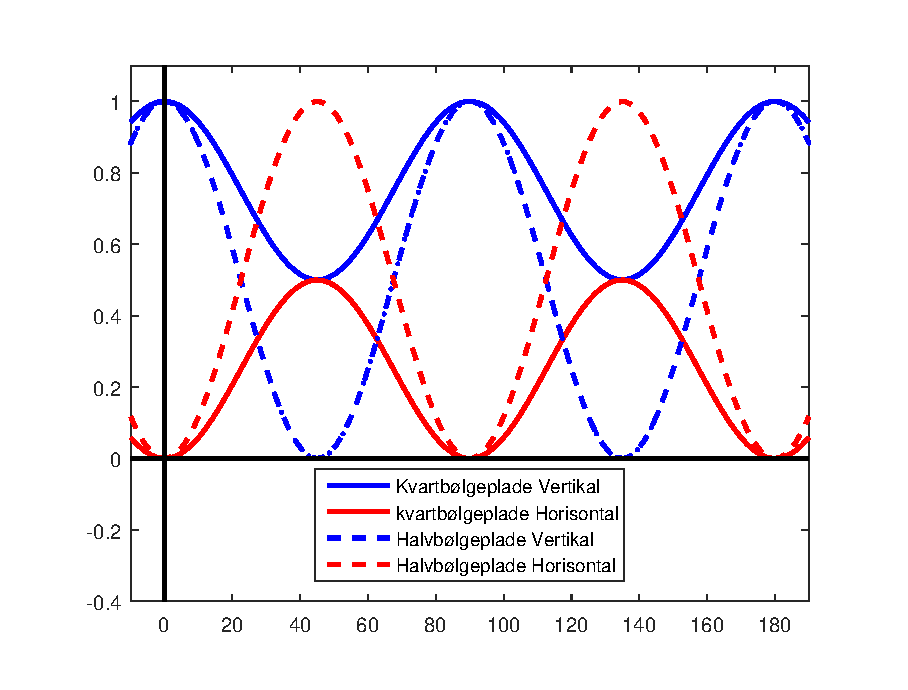
\includegraphics[width = \textwidth]{Elektrodynamik/faseskitse.eps}
\end{opgave}
 
%\chapter{Fejl}

\section{Astrofysik}
\section{Laserfysik}


\backmatter

%\printbibliography % BibLaTeX

%\bibliography{bach}{} % ikke BibLaTeX
%\bibliographystyle{alpha} % ikke BibLaTeX

\end{document}

